% Se pre-carga la información del estudiante sólo para poder emplear el macro de
% selección de versión (digital o impresa)
% ===============================================================================
% El estudiante debe llenar sus datos en esta sección para que la plantilla los 
% auto-importe y genere automáticamente las páginas de portada y de firmas 
% autorizadas.
% ===============================================================================
% Datos del estudiante:
% -------------------------------------------------------------------------------
% Nombre completo
\def \nombreestudiante {Luis Genaro Álvarez Sulecio}
% Carné
\def \uvgcarne {20168}
% Facultad
\def \uvgfacultad {Ingeniería}
% Carrera
\def \uvgcarrera {Ingeniería Mecatrónica}

% Datos del trabajo:
% -------------------------------------------------------------------------------
% Título completo
\def \titulotesis {Diseño e implementación de un sistema hidropónico automático de técnica NFT para el cultivo de cilantro en un contexto urbano}
% Año de entrega
\def \anoentrega {2024}
% Asesor
\def \nombreasesor {Ing. Pedro Joaquín Castillo Coronado}

% Datos del tribunal examinador:
% -------------------------------------------------------------------------------
% Nombre del primer examinador
\def \nombreprimerex {MSc. Carlos Esquit}
% Nombre del segundo examinador
\def \nombresegundoex {Ing. Luis Pedro Montenegro}
% Año de aprobación
\def \anoaprobacion {2021}
% Mes de aprobación
\def \mesaprobacion {diciembre }
% Día de aprobación
\def \diaaprobacion {5 }

% Capítulos pre-definidos
% -------------------------------------------------------------------------------
% Comentar las líneas de las secciones que desean omitirse, por defecto se 
% se incluyen todas.
\def \CAPprefacio {Prefacio}
\def \CAPantecedentes {Antecedentes}
\def \CAPalcance {Alcance}
\def \CAPanexos {Anexos}
\def \CAPglosario {Glosario}

% Formato y estilo de la plantilla
% -------------------------------------------------------------------------------
% Modo impresión: Puede des-comentar la siguiente línea para generar un documento pdf sin la portada, para cuando se desee imprimir el documento para encuadernación
% \def \printver {Versión del documento para impresión}

% Portada: Puede cambiarse la imagen en la portada al cambiar el nombre del 
% archivo siguiente. NOTA: debe tener la suficiente resolución para cubrir el área
% designada
\def \imagenportada {plantilla/portadacit.jpg}

% Referencias: Puede des-comentar la siguiente línea para utilizar el formato de referencias APA
%\def \usarAPA {Usar formato APA}

% Párrafo: Puede comentar la siguiente línea si desea emplear un formato de 
% párrafo distinto al establecido por defecto
\def \parpordefecto {Formato de párrafo por defecto}

% Capítulos y secciones: Puede des-comentar la siguiente línea para establecer el
% formato de los capítulos y secciones bajo el estándar original de UVG para
% trabajos de graduación. Este incluye: capítulos con numeración romana, secciones
% con letras mayúsculas, sub-secciones con números y sub-sub-secciones con letras
% minúsculas
%\def \capsecuvg {Formato UVG para capítulos y secciones}

\ifdefined\printver
    \documentclass[11pt, letterpaper, twoside, openright]{report}
\else
    \documentclass[11pt, letterpaper]{report}
\fi

% Eliminar la opción de twoside y openright si se desea generar la versión
% digital del documento en lugar de la versión impresa
%\documentclass[11pt, letterpaper, twoside, openright]{report}
\usepackage[spanish, es-nodecimaldot, es-noquoting]{babel}
% cambiar a spanish, mexico si se quiere emplear tabla en lugar de cuadro
\selectlanguage{spanish}
\usepackage[utf8]{inputenc}
\usepackage[T1]{fontenc}

\title{Plantilla para Trabajos de Graduación IE-MT 2019v4}
\author{MSc. Miguel Zea}
\date{\today}

% Información del estudiante en el archivo datos_estudiante.tex
% ===============================================================================
% El estudiante debe llenar sus datos en esta sección para que la plantilla los 
% auto-importe y genere automáticamente las páginas de portada y de firmas 
% autorizadas.
% ===============================================================================
% Datos del estudiante:
% -------------------------------------------------------------------------------
% Nombre completo
\def \nombreestudiante {Luis Genaro Álvarez Sulecio}
% Carné
\def \uvgcarne {20168}
% Facultad
\def \uvgfacultad {Ingeniería}
% Carrera
\def \uvgcarrera {Ingeniería Mecatrónica}

% Datos del trabajo:
% -------------------------------------------------------------------------------
% Título completo
\def \titulotesis {Diseño e implementación de un sistema hidropónico automático de técnica NFT para el cultivo de cilantro en un contexto urbano}
% Año de entrega
\def \anoentrega {2024}
% Asesor
\def \nombreasesor {Ing. Pedro Joaquín Castillo Coronado}

% Datos del tribunal examinador:
% -------------------------------------------------------------------------------
% Nombre del primer examinador
\def \nombreprimerex {MSc. Carlos Esquit}
% Nombre del segundo examinador
\def \nombresegundoex {Ing. Luis Pedro Montenegro}
% Año de aprobación
\def \anoaprobacion {2021}
% Mes de aprobación
\def \mesaprobacion {diciembre }
% Día de aprobación
\def \diaaprobacion {5 }

% Capítulos pre-definidos
% -------------------------------------------------------------------------------
% Comentar las líneas de las secciones que desean omitirse, por defecto se 
% se incluyen todas.
\def \CAPprefacio {Prefacio}
\def \CAPantecedentes {Antecedentes}
\def \CAPalcance {Alcance}
\def \CAPanexos {Anexos}
\def \CAPglosario {Glosario}

% Formato y estilo de la plantilla
% -------------------------------------------------------------------------------
% Modo impresión: Puede des-comentar la siguiente línea para generar un documento pdf sin la portada, para cuando se desee imprimir el documento para encuadernación
% \def \printver {Versión del documento para impresión}

% Portada: Puede cambiarse la imagen en la portada al cambiar el nombre del 
% archivo siguiente. NOTA: debe tener la suficiente resolución para cubrir el área
% designada
\def \imagenportada {plantilla/portadacit.jpg}

% Referencias: Puede des-comentar la siguiente línea para utilizar el formato de referencias APA
%\def \usarAPA {Usar formato APA}

% Párrafo: Puede comentar la siguiente línea si desea emplear un formato de 
% párrafo distinto al establecido por defecto
\def \parpordefecto {Formato de párrafo por defecto}

% Capítulos y secciones: Puede des-comentar la siguiente línea para establecer el
% formato de los capítulos y secciones bajo el estándar original de UVG para
% trabajos de graduación. Este incluye: capítulos con numeración romana, secciones
% con letras mayúsculas, sub-secciones con números y sub-sub-secciones con letras
% minúsculas
%\def \capsecuvg {Formato UVG para capítulos y secciones}
% ================================================================================
% En este archivo se colocan opciones adicionales para modificar el formato de la
% plantilla, para emplearse en otros tipos de documentos que no sean trabajos de
% graduación. Si usted está trabajando su tesis, NO modifique este archivo
% ================================================================================
% Capítulos pre-definidos
% --------------------------------------------------------------------------------
% Comentar las líneas de las secciones que desean omitirse, por defecto se 
% se incluyen todas.
\def \CAPportada {Portada}
\def \CAPcaratula {Caratula}
\def \CAPfirmas {Hoja de firmas}
\def \CAPindice {Índice general}
\def \CAPfiguras {Listado de figuras}
\def \CAPcuadros {Listado de cuadros}
\def \CAPresumen {Resumen}
\def \CAPabstract {Resumen}
\def \CAPintroduccion {Introducción}
\def \CAPobjetivos {Objetivos}
\def \CAPjustificacion {Justificación}
\def \CAPmarcoteorico {Marco teórico}
\def \CAPconclusiones {Conclusiones}
\def \CAPrecomendaciones {Recomendaciones}
\def \CAPbibliografia {Bibliografía}

% ==============================================================================
% DEFINICIÓN DE PAQUETES
% ==============================================================================
\usepackage{xcolor}
\usepackage{amsfonts}
\usepackage{amsmath}
\usepackage{amssymb}
\usepackage{amsthm}
\usepackage{amsfonts}
\usepackage{mathtools}
\usepackage{graphicx}
\usepackage{xfrac}
\usepackage{float}
\usepackage{mathtools}
\usepackage[hypertexnames=false]{hyperref}
% \usepackage{bookmark}
\usepackage[font=small]{caption}
\usepackage{subcaption}
%\usepackage{csquotes}
\usepackage{xpatch}
\usepackage{emptypage}
\usepackage{hyphenat}
\usepackage{fancyhdr}
\usepackage[backend=biber, style=ieee]{biblatex}
\ifdefined\usarAPA 
    \usepackage[backend=biber, style=apa]{biblatex}
\fi
\addbibresource{m-bibliografia.bib}

\usepackage[percent]{overpic}

\usepackage{chngcntr}

\ifdefined\CAPglosario
	%\usepackage[toc]{glossaries}
	\usepackage[numberedsection]{glossaries}
	\makeglossaries
    \newglossaryentry{latex}
{
    name=latex,
    description={Es un lenguaje de marcado adecuado especialmente para la creación de documentos científicos}
} 
 
\newglossaryentry{formula}
{
    name=fórmula,
    description={Una expresión matemática} 
}
\fi

% ==============================================================================
% MÁRGENES Y FORMATO GENERALES
% ==============================================================================
\usepackage[top=1in, left=1.5in, right=1in, bottom=1in]{geometry}
%Options: Sonny, Lenny, Glenn, Conny, Rejne, Bjarne, Bjornstrup
\usepackage[Sonny]{fncychap}

% ==============================================================================
% DEFINICIONES DE LA PLANTILLA
% ==============================================================================
\graphicspath{ {figuras/} }
\definecolor{uvg-green}{RGB}{17,71,52}
\newcommand{\defaultparformat}[1]{
	{\setlength{\parskip}{2ex}
     \input{#1}}
}
\ifdefined\capsecuvg
	\renewcommand\thechapter{\Roman{chapter}}
    \renewcommand\thesection{\Alph{section}}
	\renewcommand\thesubsection{\arabic{subsection}}
    \renewcommand\thesubsubsection{\alph{subsubection}}
\fi
\counterwithout{figure}{chapter}
\counterwithout{table}{chapter}
\counterwithout{equation}{chapter}

\newcommand{\blankpage}{
\newpage
\thispagestyle{empty}
\mbox{}
\newpage
}
% ==============================================================================

% Comandos definidos por el usuario en el archivo comandos_usuario.tex
\usepackage{dirtytalk}

% ==============================================================================
% CUERPO DEL TRABAJO
% ==============================================================================
\pagestyle{headings}
\begin{document}

% ==============================================================================
% PORTADA
% ==============================================================================
\ifdefined\printver
    \let\CAPportada\undefined
\fi 

\ifdefined\CAPportada
    \cleardoublepage\phantomsection
    % \pdfbookmark{Portada}{toc}
	\newgeometry{left=3cm, bottom=0in, top=1in, right=3cm}
	\pagecolor{uvg-green}
	\thispagestyle{empty}

	\color{white}
	\noindent \hrulefill \par
	\vspace{0.1in}
	\noindent \Huge \nohyphens{\titulotesis} \par
	\noindent \hrulefill \par
	\noindent
	\LARGE \nombreestudiante

	\begin{figure}[b!]
    	%\makebox[\textwidth]{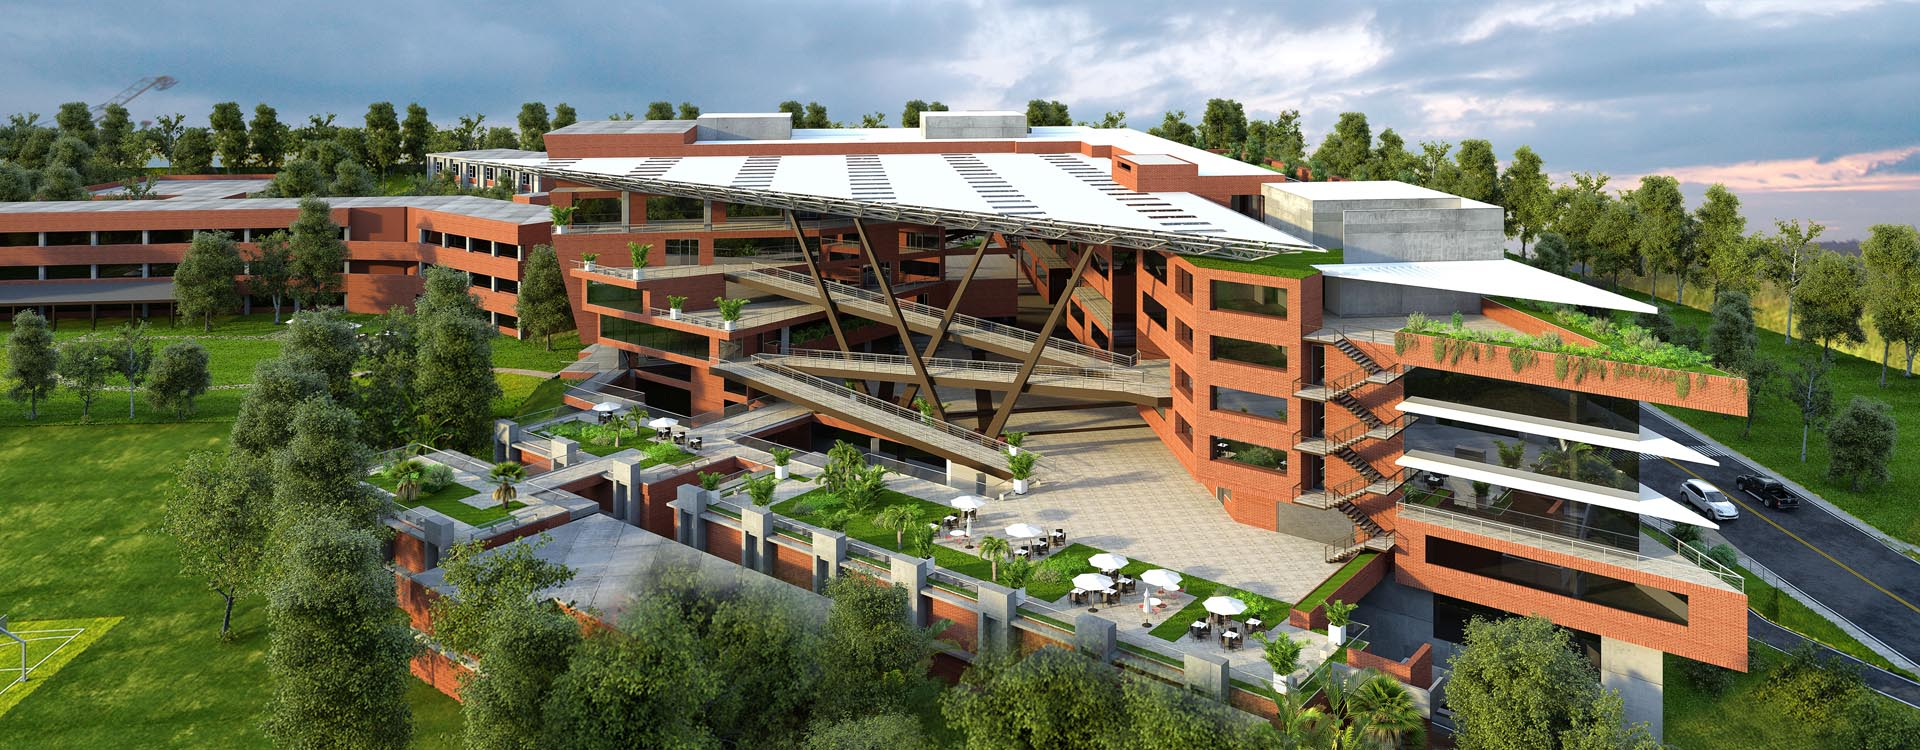
\includegraphics[height=13.25cm]{plantilla/portadacit.jpg}}
    	\makebox[\textwidth]{
    		\begin{overpic}[height=13.25cm]{\imagenportada}
     		\put(63,0){
\includegraphics[height=1.15in]{plantilla/fondologo_grande.png}}  
  			\put(64.5,2){
\includegraphics[height=0.55in]{plantilla/logoUVGblanco.eps}} 
        	\end{overpic}
    	}
    	%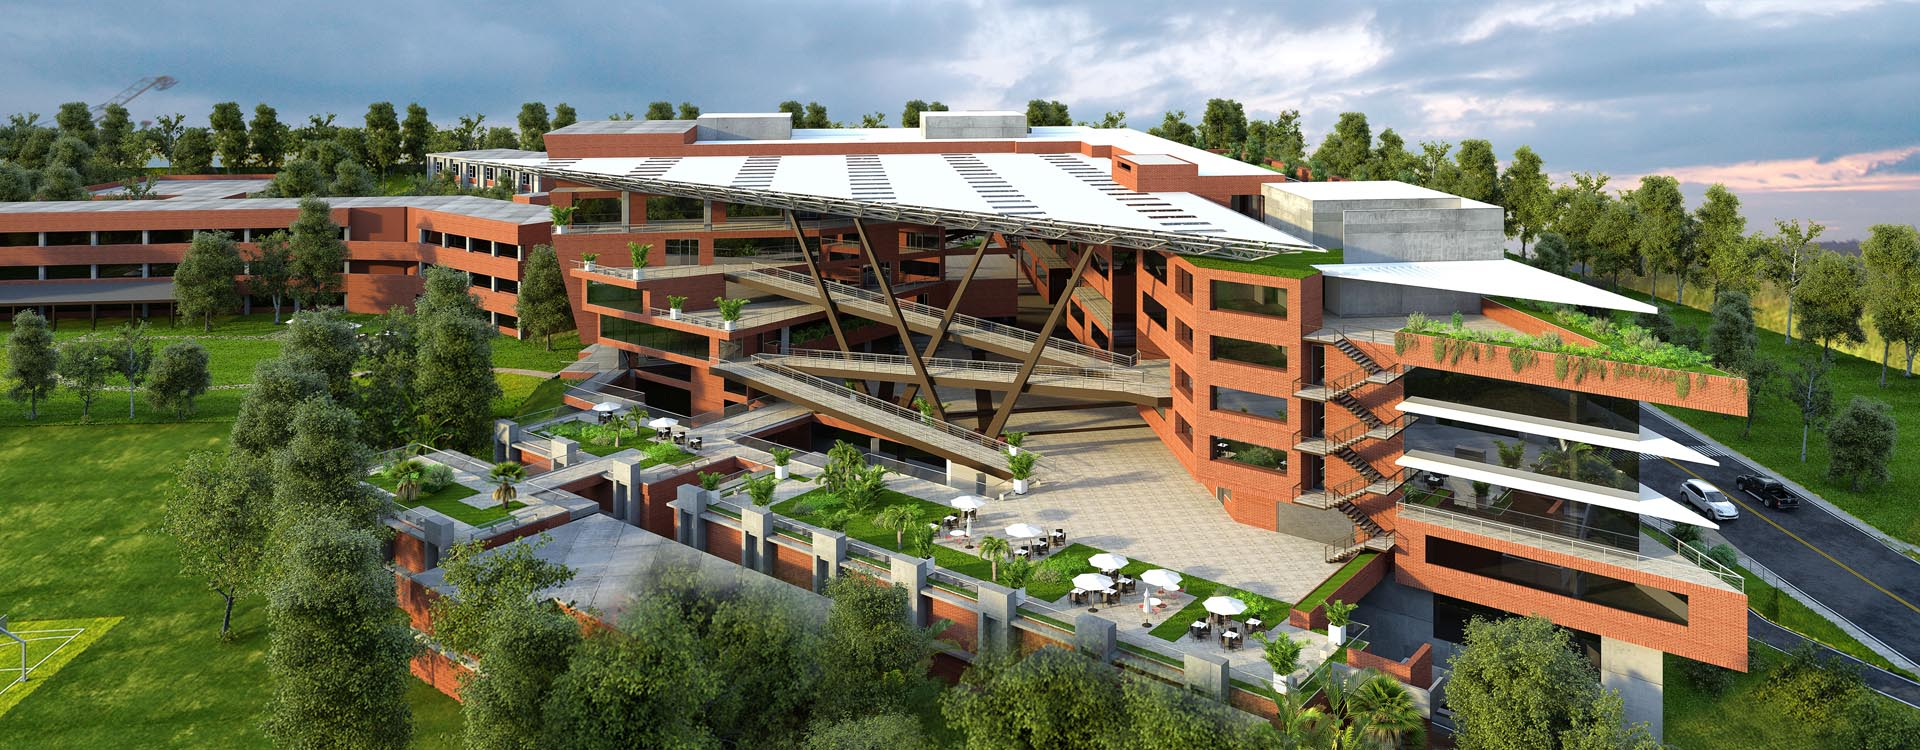
\includegraphics[height=13.25cm]{plantilla/portadacit.jpg}
	\end{figure}
	\restoregeometry
\fi

% ==============================================================================
% PRIMERAS PÁGINAS (Carátulas más hojas de guarda)
% ==============================================================================
\ifdefined\CAPcaratula
	\newpage
    \cleardoublepage\phantomsection
    % \pdfbookmark{Carátula}{toc}
	\pagecolor{white}
	\color{black}
	\setcounter{page}{1}
	\pagenumbering{roman}
	\thispagestyle{empty}
	\begin{center}
		\LARGE UNIVERSIDAD DEL VALLE DE GUATEMALA\\
		\LARGE Facultad de \uvgfacultad \\[0.75cm]
	\end{center}
	\begin{figure}[h]
		\begin{center}
		
\includegraphics[height=5.5 cm]{plantilla/escudoUVGnegro.eps}
		\vspace{0.5in}
		\end{center}
	\end{figure}
	\begin{center}
		\Large \textbf{\nohyphens{\titulotesis}} \\
		%\LARGE \textbf{\titulotesis} \\
		\vfill
		\Large \nohyphens{Trabajo de graduación presentado por \nombreestudiante \ para optar al grado académico de Licenciado en \uvgcarrera} \\
		\vfill
		\large Guatemala, \\
		\vspace{1em}
		\anoentrega
	\end{center}
    
    \ifdefined\printver	
	    \blankpage
	    \blankpage
	    
	    \newpage
	    \cleardoublepage\phantomsection
	    \pagecolor{white}
    	\color{black}
    	\setcounter{page}{1}
    	\pagenumbering{roman}
    	\thispagestyle{empty}
    	\begin{center}
    		\LARGE UNIVERSIDAD DEL VALLE DE GUATEMALA\\
    		\LARGE Facultad de \uvgfacultad \\[0.75cm]
    	\end{center}
    	\begin{figure}[h]
    		\begin{center}
    		
\includegraphics[height=5.5 cm]{plantilla/escudoUVGnegro.eps}
    		\vspace{0.5in}
    		\end{center}
    	\end{figure}
    	\begin{center}
    		\Large \textbf{\nohyphens{\titulotesis}} \\
    		%\LARGE \textbf{\titulotesis} \\
    		\vfill
    		\Large \nohyphens{Trabajo de graduación presentado por \nombreestudiante \ para optar al grado académico de Licenciado en \uvgcarrera} \\
    		\vfill
    		\large Guatemala, \\
    		\vspace{1em}
    		\anoentrega
    	\end{center}
    \fi
\fi

% ==============================================================================
% HOJA DE FIRMAS
% ==============================================================================
\ifdefined\CAPfirmas
	\newpage
	\cleardoublepage\phantomsection
	\thispagestyle{empty}
	\vspace*{0.5in}
	\large Vo.Bo.:\\[1cm]
	\begin{center}
		(f) \rule[1pt]{4 in}{1pt}\\
		\nombreasesor
	\end{center}
	\vspace{1in}

	Tribunal Examinador:\\[1cm]
	\begin{center}
		(f) \rule[1pt]{4 in}{1pt}\\
		\nombreasesor \\[1in]
		(f) \rule[1pt]{4 in}{1pt}\\
		\nombreprimerex \\[1in]
		(f) \rule[1pt]{4 in}{1pt}\\
		\nombresegundoex
	\end{center}
	\vspace{1in}

%	Fecha de aprobación: Guatemala, \rule[1pt]{0.5 in}{1pt} de \rule[1pt]{1 in}{1pt} de \anoaprobacion.
    Fecha de aprobación: Guatemala, \diaaprobacion de \mesaprobacion de \anoaprobacion.
	\normalsize
\fi

% Comentar para formato estilo libro en la numeración de páginas (NO 
% compatible con la guía UVG 2019)
\pagestyle{plain}
% ==============================================================================
% CONTENIDO DEL TRABAJO
% ==============================================================================
% PREFACIO
% ------------------------------------------------------------------------------
\ifdefined\CAPprefacio
	\newpage
	\cleardoublepage\phantomsection
    \chapter*{Prefacio}
    \ifdefined\parpordefecto
    	\defaultparformat{a-prefacio}
    \else
    	\input{a-prefacio}
    \fi
    \addcontentsline{toc}{chapter}{Prefacio}
\fi

% ÍNDICE GENERAL
% ------------------------------------------------------------------------------
\ifdefined\CAPindice
	\newpage
    \cleardoublepage\phantomsection
	\renewcommand{\contentsname}{Índice}
    %\phantomsection
    \pdfbookmark{\contentsname}{toc}
    %\pdfbookmark{Índice}{toc}
	\tableofcontents
\fi

% LISTADO DE FIGURAS
% ------------------------------------------------------------------------------
\ifdefined\CAPfiguras
	\newpage
    \cleardoublepage\phantomsection
	\renewcommand{\listfigurename}{Lista de figuras}
	\listoffigures
	\addcontentsline{toc}{chapter}{Lista de figuras}
\fi

% LISTADO DE CUADROS
% ------------------------------------------------------------------------------
\ifdefined\CAPcuadros
	\newpage
    \cleardoublepage\phantomsection
	\renewcommand{\listtablename}{Lista de cuadros}
	\listoftables
	\addcontentsline{toc}{chapter}{Lista de cuadros}
\fi

% RESUMEN
% ------------------------------------------------------------------------------
\ifdefined\CAPresumen
	\newpage
    \cleardoublepage\phantomsection
	\chapter*{Resumen}
	\ifdefined\parpordefecto
		\defaultparformat{b-resumen}
	\else
		La hidroponía es un método de crecimiento de plantas sin la dependencia del suelo para suministrar los nutrientes requeridos para el desarrollo de los cultivos. Esto se logra al utilizar una solución de nutrientes disueltos en agua los cuales son suministrados constantemente a las raíces de las plantas. Existe una gran variedad de implementaciones de cultivos hidropónicos los cuales se caracterizan por su bajo consumo de agua, independencia del suelo y su eficiencia en el uso de espacio.

Si bien en Guatemala este método de cultivo se está empezando a implementar en diferentes regiones y sectores, como en el área de forraje para ganado, aún se encuentra en sus etapas iniciales. A pesar de ser un proceso prometedor para mejorar la seguridad alimenticia del país, estos sistemas requieren de un control y monitoreo de alta precisión en intervalos constantes. Por esta razón, los sistemas hidropónicos presentan retos al requerir mano de obra constante y con conocimientos elevados para realizar las mediciones y los cálculos necesarios para asegurar que los cultivos reciban los nutrientes esenciales.

Este proyecto de graduación busca desarrollar e implementar un sistema hidropónico automático, que sea capaz de monitorear y controlar una gama de parámetros, como el nivel de pH del agua y densidad de nutrientes, sin intervención humana constante. Para lograr esto se realizará una implementación a escala de un sistema para cultivos hidropónicos urbanos, que sea capaz de asegurar el crecimiento de una plata de cilantro en condiciones controladas. Adicionalmente, se implementará una interfaz gráfica demostrativa para que el sistema pueda ser monitoreado y controlado de manera remota desde un dispositivo móvil aprovechando el contexto de la red de las cosas.



%La agricultura es una actividad esencial para el desarrollo de la sociedad. Ha sido uno de los pilares fundamentales de la humanidad desde el inicio de la era civilizada. Ahora bien, las metodologías de cultivo se han mantenido esencialmente iguales desde su descubrimiento y popularización. Si bien existen avances en semillas, fertilizantes, pesticidas, métodos de siembra y cosecha, el sistema agricultor sigue siendo propenso a una amplia gama de retos.

%Los sistema hidropónicos han sido estudiados y desarrollados en la búsqueda de mejorar la calidad de producción en climas y suelos de baja fertilidad. Adicionalmente, en el siglo XXI, esta metodología se ha posicionado como una posible solución a los retos de inseguridad alimenticia en todo el mundo. El principio básico de la 
	\fi
	\addcontentsline{toc}{chapter}{Resumen}
\fi

% ABSTRACT
% ------------------------------------------------------------------------------
\ifdefined\CAPabstract
	\newpage
    \cleardoublepage\phantomsection
	\chapter*{Abstract}
	\ifdefined\parpordefecto
		\defaultparformat{c-abstract}
	\else
		This is an abstract of the study developed under the
	\fi
	\addcontentsline{toc}{chapter}{Abstract}
\fi

% INTRODUCCIÓN
% ------------------------------------------------------------------------------
\ifdefined\CAPintroduccion
	\newpage
	\cleardoublepage
	\pagenumbering{arabic}
	\setcounter{page}{1}
	\chapter{Introducción}
	\ifdefined\parpordefecto
		\defaultparformat{d-introduccion}
	\else
		La hidroponía es un método de crecimiento de plantas sin la dependencia del suelo para suministrar los nutrientes requeridos para el desarrollo de los cultivos. Esto se logra al utilizar una solución de nutrientes disueltos en agua los cuales son suministrados constantemente a las raíces de las plantas. Existe una gran variedad de implementaciones de cultivos hidropónicos los cuales se caracterizan por su bajo consumo de agua, independencia del suelo y su eficiencia en el uso de espacio.

Si bien en Guatemala este método de cultivo se está empezando a implementar en diferentes regiones y sectores, como en el área de forraje para ganado, aún se encuentra en sus etapas iniciales. A pesar de ser un proceso prometedor para mejorar la seguridad alimenticia del país, estos sistemas requieren de un control y monitoreo de alta precisión en intervalos constantes. Por esta razón, los sistemas hidropónicos presentan retos al requerir mano de obra constante y con conocimientos elevados para realizar las mediciones y los cálculos necesarios para asegurar que los cultivos reciban los nutrientes esenciales.

Este proyecto de graduación busca desarrollar e implementar un sistema hidropónico automático, que sea capaz de monitorear y controlar una gama de parámetros, como el nivel de pH del agua y densidad de nutrientes, sin intervención humana constante. Para lograr esto se realizará una implementación a escala de un sistema para cultivos hidropónicos urbanos, que sea capaz de asegurar el crecimiento de una plata de cilantro en condiciones controladas. Adicionalmente, se implementará una interfaz gráfica demostrativa para que el sistema pueda ser monitoreado y controlado de manera remota desde un dispositivo móvil aprovechando el contexto de la red de las cosas.
	\fi
\fi

% ANTECEDENTES
% ------------------------------------------------------------------------------
\ifdefined\CAPantecedentes
	\newpage
	\chapter{Antecedentes}
	\ifdefined\parpordefecto
    	\defaultparformat{e-antecedentes}
    \else
    	En las últimas décadas se ha observado un movimiento global hacia sistemas de cultivo automatizados capaces de incrementar la calidad y efectividad de producción de cultivos. Factores como la urbanización, el crecimiento poblacional y el cambio climático han promovido el desarrollo de nuevas tecnologías de cultivo para reducir su consumo de agua y espacio requerido.

Uno de los sistemas más prometedores es el cultivo hidropónico. Estos cultivos requieren de entornos controlados y soluciones de fertilizantes en agua para lograr el crecimiento de hortalizas sin la necesidad de sustratos convencionales. La reducción en espacio y agua requerida para estos cultivos, así como su requisito de un control ambiental específico, han facilitado su integración con diferentes tecnologías para su automatización. Ciertas plataformas automatizadas para cultivos hidropónicos han sido desarrolladas e implementadas exitosamente. Sin embargo, en Guatemala, este campo de estudio aún se encuentra en desarrollo.

\section{La hidroponía en Guatemala}
Actualmente, el mercado de cultivos e infraestructuras hidropónicas en Guatemala sigue en sus etapas iniciales. Mientras que existen cultivos hidropónicos en diferentes sectores agro-industriales, esta metodología no ha sido ampliamente implementada.

En la Universidad del Valle de Guatemala, se realizó un estudio que buscó determinar las oportunidades de crecimiento y la demanda existente en el mercado para cultivos producidos en una granja urbana empleando metodologías hidropónicas. \cite{gonzalez_natareno2021_tesis} Dicho estudio buscó determinar la viabilidad económica de un sistema de cultivo hidropónico en Quetzaltenango mediante estudios de mercado y el diseño de un sistema para el cultivo de hortalizas de hoja. Se analizaron factores como la ubicación, espacio requerido, variedades de sistemas hidropónicos existentes, la segmentación del mercado, entre otros. Adicionalmente, se realizó un diseño preliminar de un sistema hidropónico utilizando la metodología NFT (Nutrient Film Technique) implementando una configuración de invernadero con túneles. La metodología NFT mantiene un flujo constante de agua sobre las raíces de manera que estas estén levemente cubiertas. Esta metodología mejora la oxigenación de las raíces y permite que estas absorban la cantidad necesaria de nutrientes. 

Al analizar los resultados de los estudios técnicos y financieros realizados, se determinó que existe un mercado disponible en el área de Quetzaltenango para la venta de cultivos hidropónicos. Adicionalmente, los resultados presentaron una alta rentabilidad para el proyecto con una tasa interna de retorno (TIR) de 128.07\% lo cual indica la factibilidad positiva de los sistemas hidropónicos en Guatemala. Cabe mencionar que este estudio consideró un sistema hidropónico manual en donde las variables estarían siendo controladas por un equipo de trabajo capacitado.

\begin{figure}[H]
	\centering
	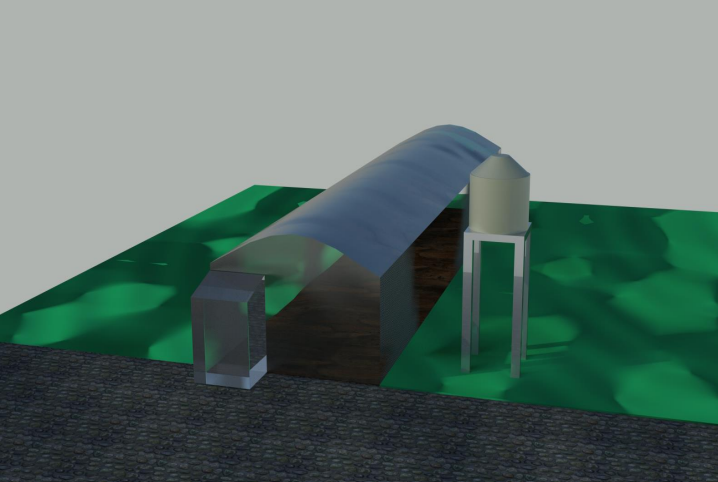
\includegraphics[scale= 0.5]{Figura1_modelo3D_invernadero_gonzalez.png}
	\caption{Modelo 3D de invernadero propuesto en estudio de factibilidad de cultivos hidropónicos.}
	\label{fig:mesh1}
\end{figure}

\section{Tendencias actuales en la producción sostenible de hortalizas}
El concepto de cultivos sin sustrato ha existido en la sociedad desde hace cientos de años. A inicios y mediados del Siglo XVII, diferentes científicos realizaron experimentos para demostrar que las plantas son capaces de crecer suspendidas en soluciones de agua, minerales y otros nutrientes. A mediados del mismo siglo, se encontró la importancia de diferentes sales las cuales ayudan a regular el proceso de crecimiento de las plantas, mejorando su rendimiento y calidad \cite{rajaseger_hydroponics_2023}. 

En la actualidad, diferentes factores como el cambio climático y el crecimiento de la población global han requerido nuevos avances en los sistemas de producción de alimentos. Estos factores han llevado a la implementación de sistemas hidropónicos en diferentes países como una medida para aumentar la producción alimenticia sin sacrificar espacio en sus territorios. Los cultivos hidropónicos presentan una gran ventaja al ser un método de cultivo altamente controlable, lo cual aumenta la productividad de un terreno. Adicionalmente, diferentes configuraciones permiten la producción de un mayor volumen de hortalizas en espacios reducidos. Junto a esto, estas metodologías reducen el impacto ambiental del cultivo de alimentos al eliminar la necesidad de alterar ecosistemas para la instalación de plantaciones masivas, y reducir el consumo de agua.

\begin{figure}[H]
	\centering
	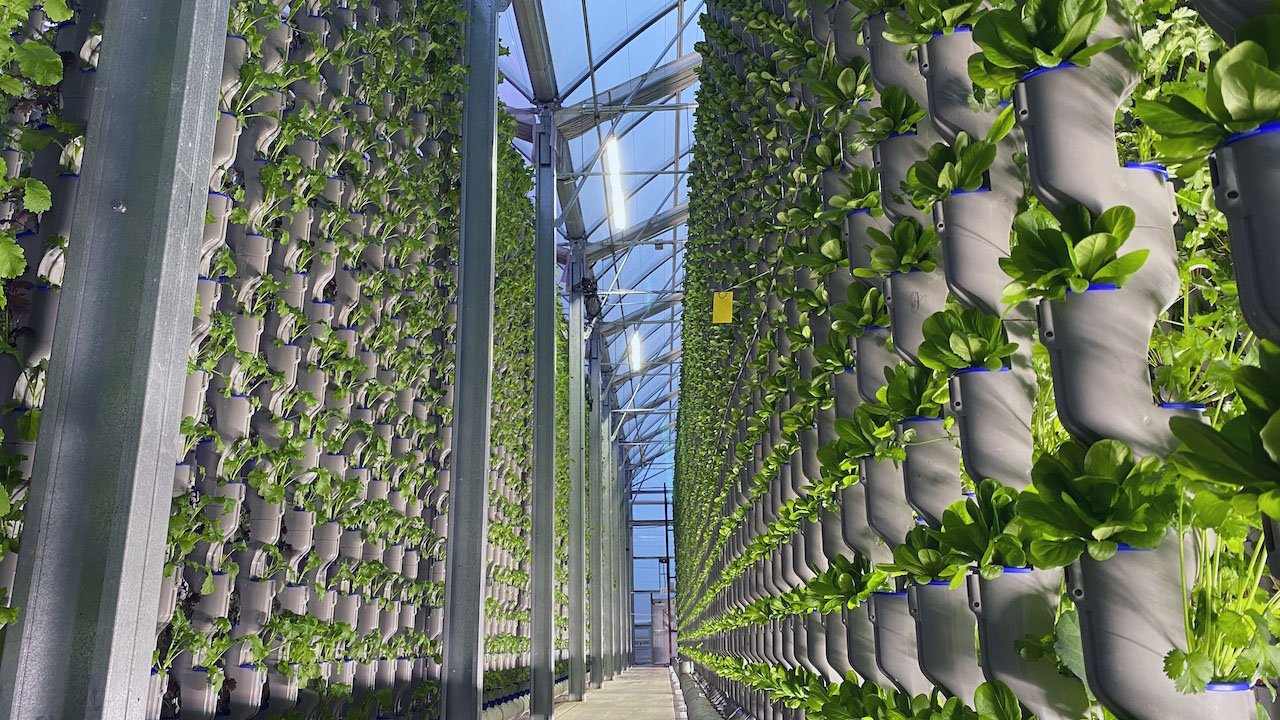
\includegraphics[scale= 0.25]{Figura3_vertical-greenhouse_edengreen.jpg}
	\caption{Granja hidropónica vertical de \textit{Eden Green}. \cite{edengreen_10_nodate}}
	\label{fig:mesh2}
\end{figure}

En el estudio de Rajaseger y colaboradores \cite{rajaseger_hydroponics_2023}, se detallaron las tendencias recientes más relevantes alrededor de la integración de cultivos hidropónicos con tecnologías inteligentes. Se destaca cómo la hidroponía es capaz de reducir el consumo de agua, minimizar el impacto ambiental de la agricultura y mejorar la calidad de los productos mientras ahorra energía y reduce tanto el espacio como la mano de obra requeridos para su producción. Adicionalmente, presenta esta tecnología como uno de los mejores candidatos para lidiar con los retos del Siglo XXI al permitir su implementación en entornos urbanos, en especial, al considerar la tendencia actual de urbanización. Se presentaron los diferentes métodos de cultivo hidropónico que se han desarrollado en los últimos años así como un resumen de los desarrollos tecnológicos en la integración de agricultura inteligente e hidroponía. Se detalló cómo varios estudios, buscando determinar la factibilidad de la hidroponía para producción sostenible, han incorporado diferentes sensores para medir características como niveles de oxígeno o pH en el agua. Estos componentes, junto con sistemas de control, permiten monitorear una gran cantidad de variables internas y externas, y controlarlas para obtener mejores resultados. Se realizó una recopilación respecto a la importancia de diferentes medios de crecimiento sólidos y nutrientes en el desarrollo de las plantas en entornos hidropónicos. Finalmente, los autores hacen énfasis en el valor de esta nueva tecnología para la producción local de alimentos en áreas urbanas. \say{Esta estrategia novedosa podrá llegar a alterar de manera significativa el sector agricultural al incentivar la producción regional de alimentos, mejorando la seguridad alimenticia y añadiendo a metodologías de cultivo más resilientes.} (\textit{Rajaseger et al.}, 2023, p. 926)

\section{Uso de \textit{Fuzzy Logic} para el control de sistemas hidropónicos}
Los sistemas hidropónicos manejan una gran cantidad de variables las cuales deben ser controladas de tal manera que se mantengan en rangos preestablecidos. Debido a la gran variedad de plantas que se pueden cultivar en un sistema hidropónico se requieren controladores con rangos que se puedan adaptar, según el cultivo seleccionado. Los controladores que emplean \textit{fuzzy logic} son capaces de alterar sus rangos de control de manera dinámica y con facilidad. Dichos controladores permiten definir rangos de entrada los cuales pueden ser mapeados a rangos de salida. Al momento de evaluar el estado del sistema, se utilizan funciones específicas para realizar una linealización aproximada de las variables medidas. En base a estas linealizaciones se determina la compensación que debe realizar el controlador para mantener los niveles deseados. Esto permite una fácil integración con sistemas IoT (\textit{Internet of Things}) puesto que los rangos pueden ser variados por el usuario según los requisitos del sistema.

\begin{figure}[H]
	\centering
	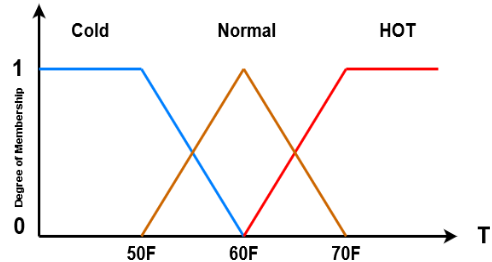
\includegraphics[scale= 0.75]{Figura4_funcion-membresia-fuzzy-logic.png}
	\caption{Función de membresía de entradas de temperatura para \textit{fuzzy logic}. \cite{thazin_iot_2019}}
	\label{fig:mesh3}
\end{figure}

\indent En el estudio de Thazin y colaboradores \cite{thazin_iot_2019}, se implementó un controlador utilizando \textit{fuzzy logic} para regular la temperatura y humedad de un sistema hidropónico mediante cambios al flujo de aire en el entorno. Se realizaron cálculos de los ventiladores DC requeridos para alterar los parámetros deseados, los cuales se instalaron en posiciones estratégicas dentro del entorno de crecimiento diseñado para mejorar el flujo de aire. Se utilizó un Arduino Nano junto con un sensor DHT22 para realizar las mediciones de temperatura y controlar la velocidad de los ventiladores. Adicionalmente, se incluyó una pantalla LCD como display para las mediciones de temperatura y velocidad de los ventiladores. Con el controlador propuesto se logró un control adecuado de la velocidad de los ventiladores en función del rango de temperatura ambiente en el área de crecimiento. Se demostró que el sistema fue capaz de variar la velocidad angular de los ventiladores utilizados según la temperatura mediante la realización de 10 pruebas a temperaturas entre los 45 y 87 °F. Adicionalmente, se logró subir los resultados a la plataforma \textit{Thing Speak} para monitorear valores de temperatura, humedad e intensidad de luz. Dicha plataforma cuenta con un servidor al cual se pueden subir datos mediante protocolos WiFi para que estos sean desplegados en gráficas en función del tiempo transcurrido.

\section{Monitoreo y control de cultivos hidropónicos utilizando tecnología IoT}
El monitoreo de las variables presentes en sistemas hidropónicos es esencial para asegurar un crecimiento óptimo de las hortalizas. Sin embargo, este proceso puede llegar a consumir mucho tiempo en el caso de sistemas a mayores escalas y puede ser ineficiente en lugares remotos. Por esta razón, el estudio de Tatas y colaboradores \cite{tatas_reliable_2022} buscó desarrollar un sistema de monitoreo y control automático de parámetros de calidad de agua y condiciones ambientales para un cultivo hidropónico en invernadero. Adicionalmente, se definió como objetivo lograr que este aprovechara tecnologías IoT para la transferencia y el análisis de datos. Se definieron requerimientos para el sistema como parámetros a monitorear, períodos de muestreo y acciones o alarmas según los diferentes eventos. Luego de la selección de los sensores que se utilizarían, en función de los parámetros que se irán a monitorear y considerando una baja frecuencia de re-calibración, se implementó una red de nodos sensoriales. Se configuró la conexión entre nodos de tal manera que todos transmitieran su señal a un solo dispositivo. Esto permitió una comunicación eficiente entre el controlador principal y los monitores de estado (sensores) sin el uso de conexiones físicas. Se realizaron mediciones de consumo eléctrico mediante las cuales se determinó un consumo máximo para la unidad principal de 11.5W bajo condiciones de alta demanda, principalmente debido a la transmisión de datos por el módulo GSM/GPRS. Luego de esto, se desarrolló un controlador implementando \textit{Fuzzy Logic} con tal de activar las bombas de circulación en los momentos adecuados. Se evaluaron los resultados tanto en pruebas de laboratorio como en el campo al instalar el sistema en un invernadero para simular condiciones reales. Se desplegaron los datos recolectados en la plataforma Ubidots y se realizaron pruebas de factibilidad del sistema. Se determinó que, tanto el sistema como los sensores, cuentan con una probabilidad de falla relativamente baja lo cual hace del sistema altamente confiable. 

\begin{figure}[H]
	\centering
	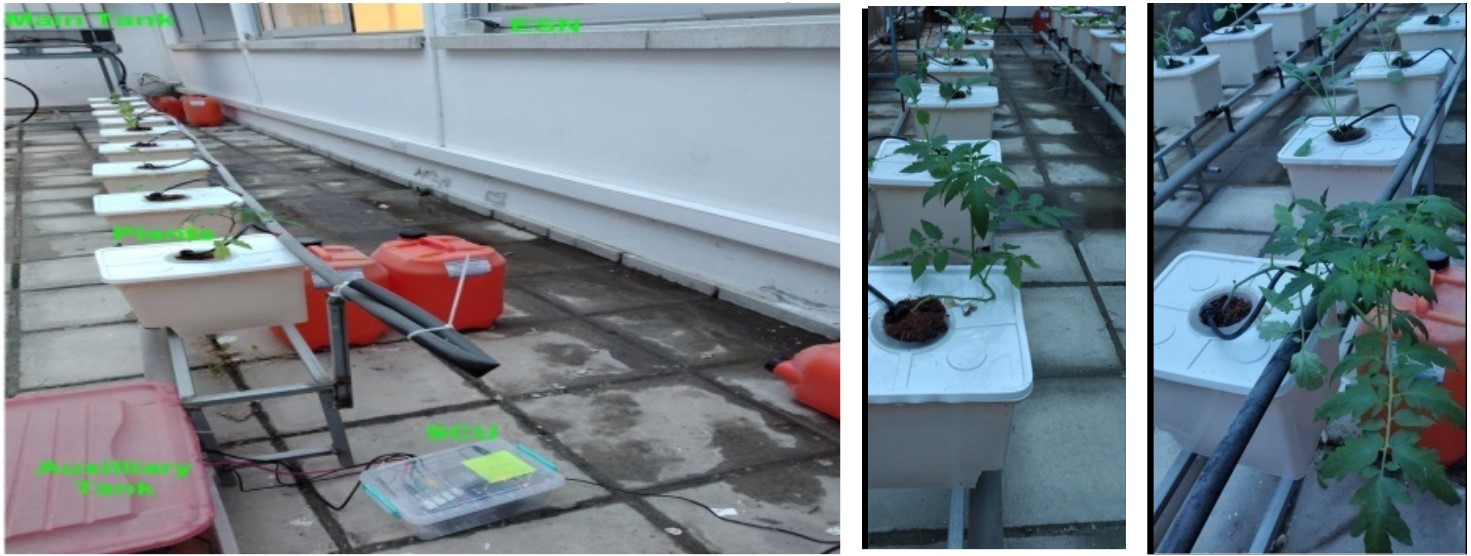
\includegraphics[scale= 0.35]{Figura2_sistema_hidroponico_en-lab_tatas.jpg}
	\caption{Sistema hidropónico implementado en condiciones de laboratorio.}
	\label{fig:mesh4}
\end{figure}

\section{La digitalización de la agricultura}
En los últimos 20 años se ha observado una tendencia hacia la automatización de la agricultura y el concepto de las granjas inteligentes \textit{Smart Farms (SF)}. Mientras que esta tendencia es bastante reciente, siendo popularizada alrededor de los años 90 del siglo pasado, se han empezado a desarrollar tecnologías que están facilitando su implementación. 
\\ En el estudio de Bacco y colaboradores \cite{bacco_digitisation_2019}, realizado en la Unión Europea en el año 2019, se analizaron las tendencias tecnológicas junto con los retos a los que se enfrenta la agricultura moderna en el contexto de la globalización y el calentamiento global. Adicionalmente, se analizaron los retos a los que se enfrentan las tecnologías de granjas inteligentes en desarrollo. Se destacaron factores como costos elevados de adopción de las tecnologías, así como falta de conectividad en áreas rurales. Así mismo, se analizaron factores técnicos y socio-económicos que están afectando la adaptación de los sistemas de agricultura tradicional a metodologías automatizadas. Un aspecto clave que se mencionó fue la tendencia de estas tecnologías hacia un sistema excesivamente industrializado, el cual tiende a desanimar a los agricultores. Sin embargo, como se menciona en el artículo, \say{-el objetivo de las granjas inteligentes (SF) no debería restringirse a la industrialización de la agricultura, sino en mejorar el proceso entero para que este sea más eficiente, sostenible y de mejor calidad, mientras que se respetan las necesidades de los agricultores.} (Bacco \textit{et al.}, 2019, p. 1), estos sistemas pueden ser diseñados de tal manera que sean más compatibles con las necesidades puntuales de los agricultores. %\vspace{10pt}
%\textit{-the aim of SF should not be just in industrializing agriculture, but in making the whole process more efficient, sustainable, and of high quality, while respecting farmers’ needs.}

\indent La hidroponía ha presentado grandes avances a lo largo de los últimos años, desde sus inicios teóricos en el Siglo XVII hasta el crecimiento en popularidad en años recientes, esta tecnología se encuentra posicionada para ser revolucionaria en la agricultura moderna. Actualmente, existen diversas empresas las cuales están demostrando los beneficios de esta tecnología junto con su viabilidad. Adicionalmente, varios estudios han comprobado su factibilidad y el potencial presente en la integración con sistemas inteligentes. El campo de la automatización agrícola se ha encontrado en crecimiento a lo largo de los últimos 20 años, y los cultivos hidropónicos presentan una plataforma idónea para su implementación en los años por venir. Tanto el calentamiento global como la urbanización han sido reconocidos como retos que pueden llegar a aumentar la falta de seguridad alimenticia en esta y futuras generaciones. Por esta razón, es de gran importancia mejorar los protocolos de automatización y sistemas de control para facilitar la adopción de los cultivos hidropónicos tanto en Guatemala como en Latinoamérica.

    \fi  
\fi

% JUSTIFICACIÓN
% ------------------------------------------------------------------------------
\ifdefined\CAPjustificacion
	\newpage
	\chapter{Justificación}
	\ifdefined\parpordefecto
		\defaultparformat{f-justificacion}
	\else
		La hidroponía ofrece grandes beneficios entre ellos, el ahorro significativo de agua, espacio de crecimiento y un control más robusto de las características de crecimiento del cultivo deseado. Ahora bien, estos sistemas requiere de cuidados específicos y diferentes a los de la agricultura tradicional, como el monitoreo de acidez o alcalinidad de la solución o su concentración de oxígeno. Como lo han demostrado varios estudios en el extranjero, contar con un sistema de regulación de parámetros autónomo permite obtener mejores resultados con sistemas hidropónicos. 

Este trabajo de graduación busca establecer una plataforma que pueda ser utilizada para analizar la viabilidad de sistemas hidropónicos automáticos para reforzar la producción de hortalizas locales, e incentivar su cultivo en contextos urbanos. Se desarrollará un sistema capaz de medir y controlar las diversas variables involucradas en el crecimiento de plantas con metodologías hidropónicas. Esta tecnología será validada mediante un prototipo del sistema a pequeña escala, diseñado con la intención de que sea adoptado en entornos urbanos para mejorar la calidad de las hortalizas consumidas. Mientras que el enfoque principal del trabajo recaerá en diseñar un sistema de bajo consumo eléctrico con costos reducidos, se buscará también optimizar la productividad del sistema. Adicionalmente, establecerá una línea base para futuras investigaciones que deseen aprovechar el control autónomo de parámetros para cultivos hidropónicos a grande y mediana escala. 

Se espera que el desarrollo de un sistema que cumpla con estas características, junto con los bajos requisitos de trabajo manual, aumente la atractividad de los sistemas hidropónicos en el mercado guatemalteco. Este tipo de sistemas serán esenciales para asegurar una producción estable de hortalizas en Guatemala, sin el riesgo pérdidas por cambios en condiciones climáticas. 
	\fi
\fi

% OBJETIVOS
% ------------------------------------------------------------------------------
\ifdefined\CAPobjetivos
	\newpage
	\chapter{Objetivos}
	\ifdefined\parpordefecto
		\defaultparformat{g-objetivos}
	\else
		\section{Objetivo General}
Diseñar e implementar un sistema hidropónico automático capaz de mantener una producción de hortalizas en un contexto urbano con espacio reducido.

\section{Objetivos específicos}
\begin{itemize}
	\item Diseñar e implementar un sistema hidropónico automático de dimensiones compactas con monitoreo y regulación de parámetros del agua. 
	\item Comparar las características de crecimiento del cilantro en el sistema hidropónico automático contra una metodología tradicional.
	\item Integrar el sistema hidropónico automático con una aplicación móvil para un monitoreo remoto de parámetros.
\end{itemize}

	\fi
\fi

% ALCANCE
% ------------------------------------------------------------------------------
\ifdefined\CAPalcance
	\newpage
	\chapter{Alcance}
	\ifdefined\parpordefecto
    	\defaultparformat{h-alcance}
    \else
    	

El presente proyecto de graduación buscó establecer las bases para el desarrollo y análisis de métodos de cultivo automático utilizando técnicas de hidroponía en la Universidad del Valle de Guatemala. Se realizó un estudio de las características de los sistemas hidropónicos, haciendo enfoque en la metodología de solución nutritiva re-circulante o NFT por sus siglas en inglés. Utilizando la información recopilada, se buscó desarrollar un prototipo que permitiera controlar diferentes parámetros relacionados al crecimiento de las plantas. Junto al desarrollo de un prototipo preliminar, se realizó una comparación de diferentes indicadores de crecimiento del cultivo seleccionado, tanto en el entorno hidropónico como en uno tradicional. Finalmente, se desarrolló una aplicación sencilla la cual permitiera monitorear los parámetros del sistema.
    \fi 
\fi

% MARCO TEÓRICO
% ------------------------------------------------------------------------------
\ifdefined\CAPmarcoteorico
	\newpage
	\chapter{Marco teórico}
	\ifdefined\parpordefecto
		\defaultparformat{i-marco_teorico}
	\else
		\section{Cultivos hidropónicos}
Históricamente, la agricultura tradicional ha utilizado el suelo como medio principal para el crecimiento de plantas gracias a su alta concentración de minerales y nutrientes esenciales para el desarrollo de hojas y frutos. Debido al crecimiento poblacional observado en los últimos siglos, las metodologías de agricultura tradicional han extraído una cantidad considerable de nutrientes del suelo, reduciendo su productividad y aumentando su dependencia de fertilizantes añadidos. 

A mediados del siglo pasado, se empezaron a investigar una técnicas de agricultura con tal de eliminar la dependencia del suelo para el crecimiento de las plantas. Una de las soluciones encontradas fueron los cultivos hidropónicos los cuales no dependen de un sustrato para entregar minerales y nutrientes esenciales para el crecimiento de las plantas, sino se aprovechan de una solución de estos en agua para maximizar la absorción por medio de las raíces \cite{raviv_soilless_2019}. Los sistemas hidropónicos se caracterizan por su bajo consumo de agua, alta eficiencia de espacio y altos niveles de productividad. Se destaca que estos sistemas no dependen de las condiciones climáticas de la región, al encontrarse en un entorno controlado, como un invernadero. Esto permite una producción constante a lo largo del año la cual no es susceptible a sequías o inundaciones. Adicionalmente, al no depender del suelo, estos sistemas se pueden expandir de manera vertical, lo cual aumenta la producción de plantas por metro cuadrado utilizado. Estas características han vuelto a la hidroponía una de las soluciones más prometedoras en el contexto del crecimiento urbano y poblacional visto en el siglo XXI. Otra de las grandes ventajas de contar con un entorno cerrado y controlable, es que los cultivos hidropónicos raras veces se encuentran expuestos a pestes o enfermedades relacionadas al suelo. Sin embargo, su dependencia de un control constante y riguroso de parámetros, hace de esta metodología de cultivo susceptible a pérdidas por mal manejo del sistema \cite{raviv_soilless_2019}.

\section{Solución nutritiva re-circulante (NFT)}
La hidroponía cuenta con una gran variedad de métodos ideados con la finalidad de maximizar espacio, eficiencia de distribución de materiales y otros parámetros de crecimiento de las plantas \cite{rajaseger_hydroponics_2023}. La principal diferencia entre los métodos de cultivo hidropónico consiste en los métodos de irrigación. El método de solución nutritiva re-circulante (\textit{Nutrient Film Technique}), también conocido como método NFT, utiliza un sistema de irrigación que genera una película delgada de agua con nutrientes que fluye sobre las raíces de las plantas. Tradicionalmente, estos sistemas se implementan con una serie de canaletas o tuberías colocadas a una inclinación de entre 0.3\% y 2\% \cite{van_os_technical_2019}. Una de las características más retadoras del método NFT consiste en el control de parámetros, como lo son los niveles de pH de la solución, su temperatura, oxígeno disuelto y saturación de nutrientes \cite{baiyin_flow_rate_2021}. Adicionalmente, varios estudios han demostrado que la tasa de flujo de la solución en el sistema se encuentra fuertemente relacionada con el rendimiento del crecimiento de las plantas. En el caso de las lechugas, Al-Tawaha y colaboradores encontraron que un flujo de 20 L/minuto fue óptimo para el desarrollo de las plantas, llevando a un mayor rendimiento \cite{al-tawaha_flow_rate_nft_2018}. Finalmente, es importante destacar que este sistema requiere que las plantas sean germinadas en un espacio separado, antes de que puedan ser introducidas al sistema.

\begin{figure}[H]
	\centering
	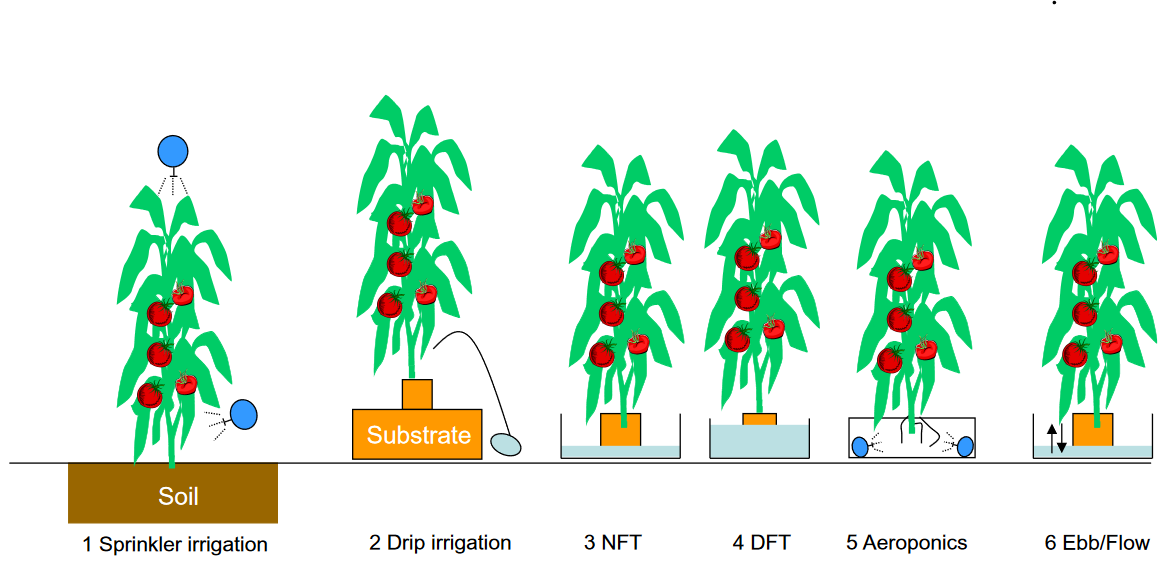
\includegraphics[scale= 0.35]{Figura_5_metodos_irrigacion.png}
	\caption{Variedad de métodos de irrigación para cultivos \cite{van_os_technical_2019}.}
	\label{fig:mesh5}
\end{figure}

\begin{figure}[H]
	\centering
	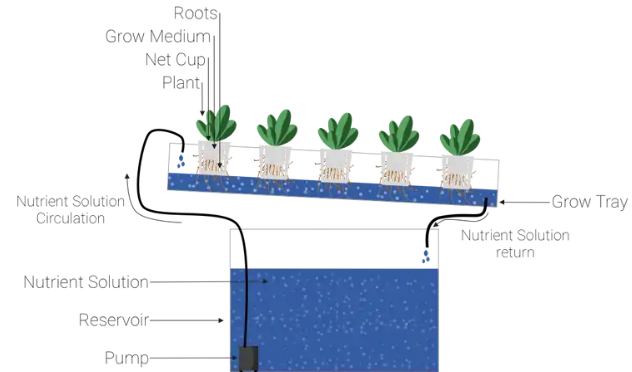
\includegraphics[scale= 0.45]{Figura_6_sistema_nft.png}
	\caption{Diagrama simplificado de metodología NFT para cultivos hidropónicos \cite{NutrientFilmTechnique_2023}.}
	\label{fig:mesh6}
\end{figure}

\section{Solución de nutrientes}
Acceso constante a luz solar, agua, oxígeno y dióxido de carbono es esencial para la supervivencia de las plantas. Sin embargo, esto no es lo único que requieren para su crecimiento. Normalmente, las plantas obtienen la mayoría de los minerales y nutrientes necesarios para su crecimiento del suelo, el cual, a lo largo de varios años por procesos naturales, ha acumulado en diferentes cantidades. Las plantas requieren de 13 nutrientes minerales necesarios para su desarrollo y crecimiento adecuado. Sus características de crecimiento y la calidad de las plantas estarán definidas por el porcentaje de nutrientes que tengan disponibles y que sean capaces de absorber \cite{marulanda_huerta_2003}. Estos nutrientes se pueden dividir en tres categorías según la función que cumple cada elemento. La primera categoría se conoce como los macro-nutrientes, estos son nutrientes que las plantas requieren en altas cantidades pues son esenciales para el desarrollo de las estructuras fundamentales para su crecimiento. En este grupo se encuentran el Nitrato requerido para el desarrollo de hojas y tallos; el Fósforo, requerido para el desarrollo de raíces, la formación de semillas y la maduración de frutos; y el Potasio, requerido para el desarrollo de frutos y la acumulación de nutrientes en la planta \cite{marulanda_huerta_2003}.

La segunda categoría consiste en minerales requeridos para el correcto desarrollo de la planta, sin embargo, estos son requeridos en cantidades más bajas por lo que se conocen como elementos secundarios. Entre estos se encuentra el Calcio, el cual activa la formación de raíces, especialmente en las primeras etapas de desarrollo y neutraliza las sustancias tóxicas producidas por la planta. También se encuentra el Azufre, el cual es esencial en la producción de proteínas, mejora el crecimiento de la planta y facilita el desarrollo de semillas. Adicionalmente, en este grupo se cuenta con el Magnesio, el cual es fundamental para las plantas porque es requerido para la creación de clorofila y las azúcares que requieren para vivir, adicionalmente es utilizado para regular los nutrientes dentro de la planta y fomenta la creación de aceites y grasas \cite{marulanda_huerta_2003}. Finalmente, se cuenta con una serie de micro-nutrientes, los cuales cumplen una gran variedad de funciones que facilitan el desarrollo de la planta y aseguran un mayor rendimiento de la misma. Estos se detallan a continuación \cite{atlas_scientific_nutrient_2023}:

\begin{itemize}
	\item Cloro\\
	Utilizado para facilitar el proceso de fotosíntesis y regular los niveles de sales y líquido en las células lo cual asegura una planta fresca y saludable.
	\item Molibdeno\\
	Elemento esencial para la fijación de nitrógeno y utilizado en el proceso de conversión de nitrato a amoniaco.
	\item Manganeso\\
	De gran utilidad para aumentar la resiliencia de las plantas ante situaciones de alto estrés, y utilizado en el proceso de activación de enzimas.
	\item Zinc\\
	Requerido para la síntesis de hormonas de crecimiento y el desarrollo de raíces.
	\item Boro\\
	Apoya en el proceso de crecimiento al fomentar la división de células y el metabolismo de carbohidrátos.
	\item Hierro\\
	Esencial para la transferencia de energía entre células y la producción de clorofila.
	\item Cobre\\
	Mejora la estructura de las plantas al reforzar las paredes celulares mediante la formación de lignina. Esencial en la creación de estructuras maderosas.
\end{itemize}

El correcto suministro y balance de estos componentes en un sistema hidropónico es esencial para asegurar el crecimiento adecuado y el rendimiento de los cultivos. Ahora bien, su aplicación y control de manera individual sería sumamente difícil, por esta razón, se han desarrollado fórmulas para proveer estos nutrientes en un sistema hidropónico. En la industria estas soluciones se conocen como solución concentrada A y B, donde la primera cuenta con los macro-nutrientes y nutrientes secundarios, mientras que la segunda cuenta con los micro-nutrientes \cite{marulanda_huerta_2003}. Estas soluciones pueden ser creadas de manera independiente, o se pueden adquirir en el mercado. Es importante destacar que los porcentajes de concentración a utilizar en el sistema hidropónico dependerá del tipo de cultivo y sus requisitos. Por ejemplo, un cultivo de hortalizas requerirá mayores porcentajes de nitrógeno y nutrientes secundarios, mientras que plantas con flores y frutos, requerirán una mayor concentración de fósforo y potasio. Así mismo, cambios en la temperatura requerirán de un ajuste en la concentración total en el agua, puesto que, a mayores temperaturas, las plantas aumentarán su consumo de agua, mas no su dependencia en minerales, mientras que a menores temperaturas, se ve lo opuesto \cite{marulanda_huerta_2003}.

\section{Características de la solución nutritiva del cilantro}
El cilantro es una hierba bastante versátil la cual requiere de una baja cantidad de nutrientes con tal de presentar una productividad significativa. De los nutrientes mencionados anteriormente, el cilantro requiere únicamente un control rigoroso de los macro-nutrientes principales así como una baja cantidad de Calcio y Magnesio \cite{letpot_nodate}. Este control de macro-nutrientes va de la mano con una regulación cuidadosa de la temperatura del agua. Esto pues, en diferentes rangos de temperatura varía la necesidad de nutrientes así como su facilidad de absorción \cite{voogt_nutrient_2019}.

Según el estudio realizado por Currey y colaboradores, uno de los factores que más interfiere en el crecimiento y desarrollo del cilantro es la cantidad de fotones que reciben las plantas durante el día. Esto se puede traducir a la cantidad de horas de luz que requieren para su crecimiento óptimo, el cual se encuentra en un rango de 12 a 16 horas de luz diarias \cite{letpot_nodate}. Una conclusión importante del estudio de Currey y colaboradores es que si bien la concentración de luz disponible para la planta aumenta su productividad, no es necesario realizar un ajuste de la densidad de nutrientes debido al aumento en concentración de luz \cite{currey_nutrient_2019}. A continuación se detallan los parámetros del agua requeridos para el correcto desarrollo del cilantro en un sistema hidropónico:

\begin{table}[H]
	\centering
	\begin{tabular}{|c|c|}
		\hline
		\multicolumn{2}{|c|}{\textbf{Características de la solución nutritiva}}\\ \hline
		Concentración de nutrientes: & 1.2 a 1.8 mS/cm \\ \hline
		Potencia de hidrógeno (pH): & 5.5 a 6.7 \\ \hline
		Temperatura del agua: & 15 a 20 °C \\ \hline
		Nutrientes requeridos: & Nitrógeno, fósforo, potasio, calcio y magnesio \\ \hline
		Concentración de nutrientes: & NPK 15:15:15\\ \hline
		Nutrientes adicionales: &  0.5\% Nitrato de calcio y 0.5\% Sulfato de magnesio\\ \hline
		Tiempo de crecimiento: & 50 a 55 días\\ \hline
		Espacio entre plantas: & 18 cm \\ \hline
	\end{tabular}
	\caption{Parámetros esenciales para el crecimiento de Cilantro en sistemas hidropónicos \cite{mondol_use_2023} \cite{letpot_nodate}.}
	\label{Cuadro0}
\end{table}

\section{Monitoreo de parámetros para el crecimiento de plantas}
Como se detalló anteriormente, los cultivos hidropónicos requieren de un control constante y preciso de una gran variedad de parámetros. El monitoreo adecuado de parámetros como el nivel de oxigenación del agua, la cantidad de nutrientes, el nivel de acidez de la solución, la temperatura del ambiente, temperatura del agua, y el nivel de humedad son esenciales para asegurar el crecimiento óptimo de las plantas. Tradicionalmente, estos parámetros se miden con una serie de pruebas químicas o sensores independientes. A continuación, se detallan los diferentes sensores que se pueden utilizar en un cultivo hidropónico para medir los parámetros del agua así como la importancia de cada uno de dichos parámetros.

\subsection{Oxígeno disuelto en agua}
Los sistemas hidropónicos se enfrentan a varios retos, entre estos, la cantidad de oxígeno disuelto en la solución de nutrientes. Este parámetro es esencial para el desarrollo saludable de las raíces, puesto que con bajos niveles de oxígeno, estas pueden experimentar una enfermedad conocida como hipoxia. Según el estudio realizado por Roosta, los niveles de oxígeno están directamente relacionados no sólo con el crecimiento de las raíces, sino también con los procesos fotosintéticos y de crecimiento de los cultivos hidropónicos. Este parámetro afecta la absorción de Nitrógeno ya sea que se encuentre en la forma de sales de nitratos o amoníacos\cite{roosta_responses_2024}. La concentración de oxígeno disuelto se mide en mg/L, lo cual se puede lograr con una gran variedad de sensores.

\subsection{\textit{SEN0237 Gravity Analog Dissolved Oxygen Sensor} de \textit{DFRobot}}
El sensor analógico de oxígeno disuelto consiste en una sonda galvánica equipada con un electrodo el cual junto con una solución de hidróxido de sodio, también conocido como sosa cáustica, es capaz de detectar la concentración de oxígeno disuelto en agua. Dicho sensor debe ser calibrado antes de que se pueda utilizar, sin embargo, dicho proceso es relativamente sencillo \cite{DFRobot_DOsensor}. 

Según el fabricante, el sensor se puede calibrar utilizando un método de punto singular o de doble punto. El primer proceso requiere de la preparación de una solución de oxígeno concentrado en agua, esto se puede lograr utilizando un batidor o con una bomba de aire inmersa en el agua destilada durante 10 minutos. Una vez terminen los 10 minutos, se espera a que dejen de salir burbujas, y se sumerge la sonda en la solución. Se mantienen mezclando la solución lentamente para evitar burbujas hasta que el nivel de voltaje se estabilice y se guardan los valores de temperatura y voltaje como punto de saturación. El proceso de doble punto es similar al descrito anteriormente, sin embargo, requiere de dos soluciones a dos temperaturas diferentes. Se recomienda que una se encuentre alrededor de 5°C y la otra entre los 35° y 38°C \cite{DFRobot_DOsensor}. 

A continuación, se detallan las características del sensor:

\begin{table}[H]
	\centering
	\begin{tabular}{|c|c|}
		\hline
		\multicolumn{2}{|c|}{\textbf{Sonda del sensor de oxígeno disuelto}}\\ \hline
		Rango de detección: & 0 a 20 mg/L \\ \hline
		Rango de temperatura: & 0 a 40 °C \\ \hline
		Tiempo de respuesta: & 90 segundos a 25 °C \\ \hline
		Rango de presión: & 0 a 50 PSI \\ \hline
		Vida útil del electrodo: & 1 año (bajo condiciones normales de uso) \\ \hline
		Tiempo de reemplazo de membrana: & Cada 4 a 5 meses en agua clara \\ \hline
		Tiempo de reemplazo de solución: & Una vez al mes \\ \hline
		Largo del cable: & 2 metros \\ \hline
		Tipo de conector de la sonda: & BNC \\ \hline
		\multicolumn{2}{|c|}{\textbf{Placa de conversión de señales del sensor}}\\ \hline 
		Voltaje de alimentación: & 3.3 a 5.5 VDC \\ \hline
		Voltaje de señal de salida: & 0 a 3.3 VDC \\ \hline
		Cable de conexión: & BNC \\ \hline
		Conector de señal: & Interfaz PH2.0 - 3 pin \\ \hline
		Dimensiones: & 42mm $\times$ 32mm (1.65in $\times$ 1.26in) \\ \hline
	\end{tabular}
	\caption{Características de funcionamiento del sensor SEN0237 de \textit{DFRobot}.}
	\label{Cuadro1}
\end{table}

\begin{figure}[H]
	\centering
	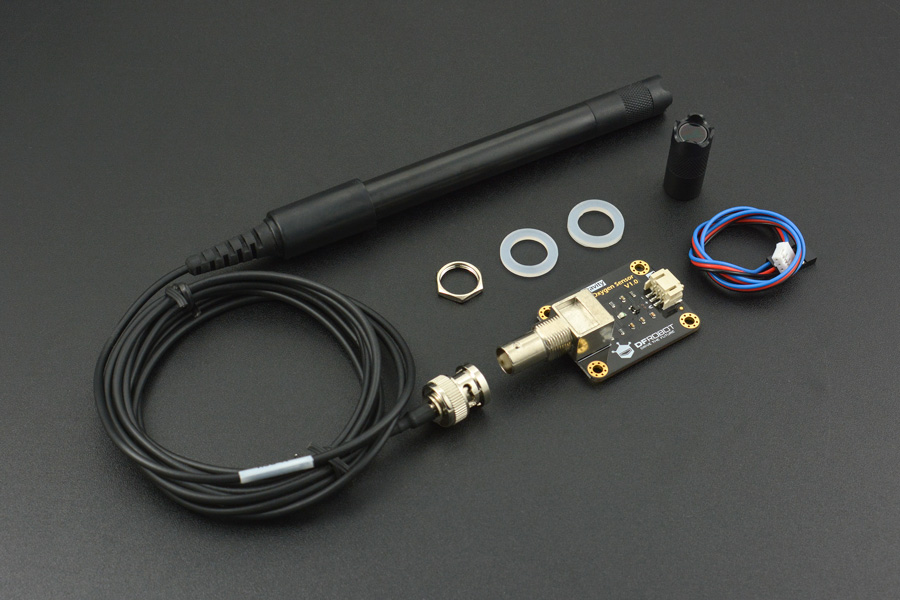
\includegraphics[scale= 0.25]{Figura_7_sensor_oxigeno.jpg}
	\caption{Sensor analógico de oxígeno disuelto \cite{DFRobot_DOsensor}.}
	\label{fig:mesh7}
\end{figure}


\subsection{Sensor de electro conductividad (EC)}
Las soluciones de nutrientes requeridas para el crecimiento de las plantas cuentan con compuestos en la forma de sales, las cuales afectan la conductividad eléctrica del agua. Estas variaciones permiten utilizar los sensores de electro conductividad para determinar de manera aproximada la concentración de solución nutritiva en el agua de riego. La conductividad, medida en mS/cm (mili sievers por centímetro), es una propiedad de los materiales la cual se define como el inverso de la resistencia. El sensor \textit{DFR0300 Gravity Analog Electrical Conductividy Sensor} de \textit{DFRobot} cuenta con dos electrodos los cuales son introducidos en el agua para determinar su conductividad eléctrica, esta señal es luego convertida a un valor de voltaje analógico y transmitido a un microcontrolador \cite{DFRobot_ECsensor}. A continuación se detallan las características del sensor:

\begin{table}[H]
	\centering
	\begin{tabular}{|c|c|}
		\hline
		\multicolumn{2}{|c|}{\textbf{Sonda del sensor de conductividad eléctrica}}\\ \hline
		Constante de celda: & 1.0 \\ \hline
		Rango de detección admisible: & 0 a 20 mS/cm \\ \hline
		Rango de detección recomendado: & 1 a 15 mS/cm \\ \hline
		Rango de temperatura: & 0 a 40 °C \\ \hline
		Vida útil del sensor: & Más de 6 meses según frecuencia de uso \\ \hline
		Largo del cable: & 100 cm \\ \hline
		\multicolumn{2}{|c|}{\textbf{Placa de conversión de señales del sensor}}\\ \hline 
		Voltaje de alimentación: & 3.0 a 5.0 VDC \\ \hline
		Voltaje de señal de salida: & 0 a 3.4 VDC \\ \hline
		Certeza de medición: & $\pm 5\%$ F.S. \\ \hline
		Cable de conexión: & BNC \\ \hline
		Conector de señal: & Interfaz PH2.0 - 3 pin \\ \hline
		Dimensiones: & 42mm $\times$ 32mm (1.65in $\times$ 1.26in) \\ \hline
	\end{tabular}
	\caption{Características de funcionamiento del sensor DFR0300 de \textit{DFRobot}.}
	\label{Cuadro2}
\end{table}

\begin{figure}[H]
	\centering
	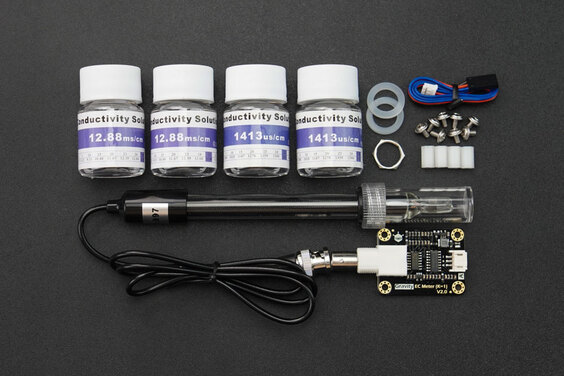
\includegraphics[scale= 0.4]{Figura_8_sensor_conductividad.jpg}
	\caption{Sensor analógico de electro conductividad \cite{DFRobot_ECsensor}.}
	\label{fig:mesh8}
\end{figure}

\subsection{Potencia de hidrógeno (pH)}
El pH o potencia de hidrógeno se conoce como la facilidad con la que una sustancia en disolución libera protones de hidrógeno o iones de oxidrilo. Según esta definición, una sustancia ácida se caracteriza por una sustancia que libera protones de hidrógeno (H+) mientras que una sustancia básica es aquella que entrega iones de oxidrilo (OH-). La escala de pH es una función logarítmica que describe la relación entre estas propiedades de una solución. Esta se encuentra en un rango de 0 a 14, en donde 0 corresponde a una sustancia ácida, mientras que 14 indica una extremadamente básica \cite{chang_quimica_1995}. La solución de agua utilizada para alimentar las plantas en un cultivo hidropónico debe contar con un pH estable, usualmente definido por el tipo de planta que se desea cultivar. En el libro \textit{Plant Factory Using Artificial Light}, el autor Wada describe cómo la regulación de pH en las soluciones nutritivas no es sólo esencial para el crecimiento de las plantas, sino también para asegurar que los nutrientes se mantengan en su estado óptimo. Wada indica que un pH por encima de 7.0 induce la presipitación del Hierro y Manganeso, lo cual afectará la producción de clorofila y volverá a las plantas más susceptibles a estrés, mientras que un pH debajo de 4.5 implicará un daño a las raíces. La regulación de los niveles de pH en sistemas hidropónicos se pueden realizar mediante mediciones de electro conductividad, para determinar los porcentajes de bicarbonato en el agua, o utilizando un sensor de pH \cite{wada_theory_2019}. Ambos métodos presentarán resultados útiles para el control de dicho parámetro, sin embargo, contar con un sensor de pH permitirá obtener una lectura directa mientras que las lecturas de conductividad únicamente indicarán el pH según las sales presentes en la solución.

\subsection{Sensor de pH \textit{SEN0161 PH Meter} de \textit{DFRobot}}
Este sensor cuenta con una construcción sencilla la cual hace de este sensor fácil de utilizar. Al ser un sensor analógico, este requiere de un proceso de calibración utilizando soluciones cuyo pH sea conocido. Cuenta con un indicador led el cual se utiliza para determinar si el sensor se encuentra encendido o no. Adicionalmente, el conector utilizado para la placa de conversión de señales permite su fácil integración con placas de desarrollo como el Arduino o ESP32 \cite{DFRobot_PHsensor}. A continuación se detallan las características del sensor:

\begin{table}[H]
	\centering
	\begin{tabular}{|c|c|}
		\hline
		\multicolumn{2}{|c|}{\textbf{Sonda del sensor de pH}}\\ \hline
		Rango de detección: & 0 a 14 pH \\ \hline
		Rango de temperatura: & 0 a 60 °C \\ \hline
		Tiempo de respuesta: & Menor o igual a 1 minuto \\ \hline
		\multicolumn{2}{|c|}{\textbf{Placa de conversión de señales del sensor}}\\ \hline 
		Voltaje de alimentación: & 5.0 VDC \\ \hline
		Cable de conexión & BNC \\ \hline
		Conector de señal: & Interfaz PH2.0 - 3 pin \\ \hline
		Certeza de medición: & $\pm 0.1$pH a 25 °C. \\ \hline
		Dimensiones: & 42 mm $\times$ 32 mm (1.65 in $\times$ 1.26 in) \\ \hline
		Potenciómetro de ajuste de ganancia & Sí \\ \hline
		Indicador de potencia: & LED \\ \hline
		Largo del cable: & 660mm \\ \hline
	\end{tabular}
	\caption{Características de funcionamiento del sensorSEN0161 de \textit{DFRobot}.}
	\label{Cuadro3}
\end{table}

\begin{figure}[H]
	\centering
	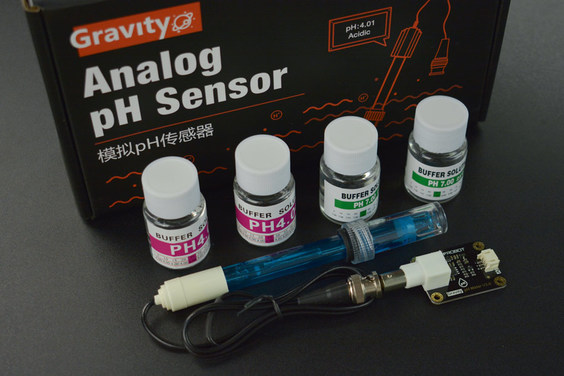
\includegraphics[scale= 1.5]{Figura_9_sensor_ph.jpg}
	\caption{Sensor analógico de potencia de hidrógeno (pH) \cite{DFRobot_PHsensor}.}
	\label{fig:mesh9}
\end{figure}

\subsection{Temperatura de agua}
La temperatura del agua es de gran importancia para las plantas puesto que está directamente relacionado a la capacidad de absorción de nutrientes. Esta temperatura es de especial importancia en las raíces, puesto que variaciones en la temperatura de estas afecta tanto la micro-biología que se desarrolle en las raíces como la habilidad de las mismas para absorber nutrientes. Adicionalmente, la temperatura afectará la precisión de lecturas de electro conductividad así como pH y oxígeno disuelto \cite{voogt_nutrient_2019}. Es por esta razón que la lectura y el control adecuado de la temperatura del agua es esencial en un sistema hidropónico. 

\subsection{Sensor de temperatura de agua DS18B20}
Uno de los sensores más fáciles de utilizar es el sensor de temperatura tipo sonda DS18B20. Este sensor utiliza el protocolo de comunicación 1-wire, lo cual reduce considerablemente la complejidad de conexión y la transmisión de datos. A continuación se detallan sus características \cite{la_electronica_DS18B20}:

\begin{table}[H]
	\centering
	\begin{tabular}{|c|c|}
		\hline
		\multicolumn{2}{|c|}{\textbf{Sonda del sensor de pH}}\\ \hline
		Rango de medición: & -55 a 125 °C \\ \hline
		Voltaje de operación: & 3.5 a 5.0 VDC \\ \hline
		Protocolo de comunicación: & 1-wire \\ \hline
		Resolución programable: & 9 a 12 bits \\ \hline
		Largo de cable: & 1 metro \\ \hline
	\end{tabular}
	\caption{Características de funcionamiento del sensor DS18B20.}
	\label{Cuadro4}
\end{table}

\begin{figure}[H]
	\centering
	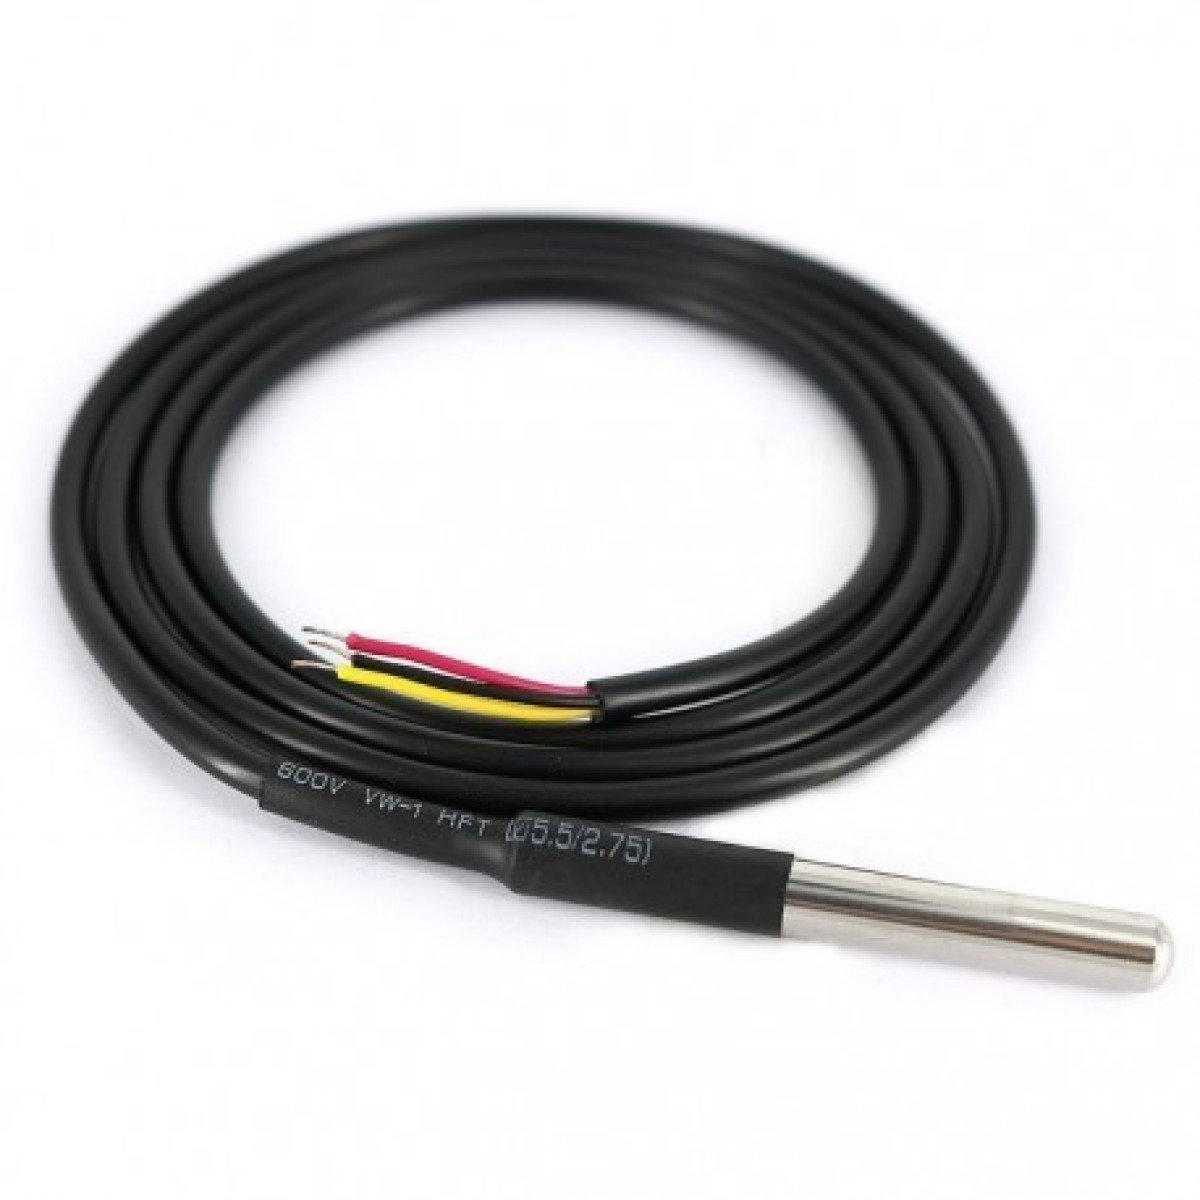
\includegraphics[scale = 0.15]{Figura_10_sensor_temperatura.jpg}
	\caption{Sensor tipo sonda de temperatura del agua \cite{la_electronica_DS18B20}.}
	\label{fig:mesh10}
\end{figure}

\subsection{Temperatura y humedad ambiental}
Las plantas son organismos particularmente susceptibles a las condiciones ambientales, tanto a los niveles de luz como a la temperatura y humedad disponible. Estos parámetros afectan diferentes procesos de las plantas, desde la absorción de nutrientes hasta el desarrollo de las hojas. Según el estudio realizado por Chia y Lim, la humedad ambiental presentó un impacto significativo en el desarrollo de cultivos, donde se observó un aumento en la masa de las plantas luego de su cosecha \cite{chia_critical_2022}. Los autores describen como las plantas en un rango de humedad relativa (RH) alrededor del 85\% presentan un aumento en su masa seca. Destacaron que a mayores porcentajes de humedad, las plantas presentan dificultades con las razones de transpiración, regulación de agua, desarrollo de área superficial de las hojas y una disminución en absorción de nutrientes. Por otro lado, destacaron que a menores concentraciones de humedad, las plantas aumentan su consumo de agua junto con sus tazas de transpiración, lo cual puede presentar un riesgo en plantas que presentan dificultades en el control de las aperturas estomáticas, lo cual afecta los procesos de fotosíntesis \cite{chia_critical_2022}.

Al igual que la humedad ambiental, la temperatura del aire alrededor de las plantas afectará su crecimiento. En el estudio realizado por Rusu y colaboradores, se analizó el crecimiento de plantas de albahaca bajo condiciones controladas con tal de determinar el impacto de dichos parámetros en el desarrollo de las plantas. Se estableció que si bien el control de la temperatura de la solución es esencial para el correcto desarrollo delas plantas, la temperatura del ambiente es igual de importante. Esto se debe a que la temperatura ambiental afectará los procesos de transpiración de las plantas, el proceso de fotosíntesis, la conductividad estomática y el crecimiento de las estructuras de la planta \cite{rusu_overview_2021}. Por otro lado, ciertos compuestos bioactivos aumentan en concentración al estar en rangos de temperatura elevados (mayores a 30° C). Finalmente, los extremos de temperatura presentan un aumento en el estrés de las plantas, llevando a una mayor demanda de agua, lo cual puede aumentar la concentración de sales creando bloqueos \cite{bita_plant_2013}. 

\subsection{Sensor de temperatura y humedad DHT11}
El sensor DHT11 es uno de los sensores más básicos y de bajo costo disponibles en el mercado para la medición de temperatura y humedad relativa en el entorno. Cuenta con un sensor capacitivo el cual es capaz de detectar el porcentaje de humedad relativo en el aire, así como una termo-resistencia la cual es capaz de detectar cambios en la temperatura ambiental. \cite{adafruit_dht11} Este sensor utiliza el protocolo \textit{one-wire} lo cual minimiza los puertos a utilizar, y elimina la necesidad de puertos analógicos para realizar lecturas. Ahora bien, cuenta con un período de muestreo máximo de una lectura por segundo, lo cual hace que sea poco preciso en ambientes con alta variabilidad. A continuación se detallan las características del sensor.

\begin{table}[H]
	\centering
	\begin{tabular}{|c|c|}
		\hline
		\multicolumn{2}{|c|}{\textbf{Sensor DHT11}}\\ \hline
		Rango de medición de temperatura: & 0 a 50 °C \\ \hline
		Precisión de temperatura: & $\pm$ 2° C \\ \hline
		Rango de medición de humedad: & 20 a 80\% \\ \hline
		Precisión de humedad: & 5\% \\ \hline
		Voltaje de operación: & 3.0 a 5.0 VDC \\ \hline
		Corriente máxima: & 2.5mA \\ \hline
		Frecuencia de muestreo: & 1Hz \\ \hline
		Protocolo de comunicación: & \textit{1-wire} \\ \hline
	\end{tabular}
	\caption{Características de funcionamiento del sensor DHT11 \cite{adafruit_dht11}.}
	\label{Cuadro5}
\end{table}

\begin{figure}[H]
	\centering
	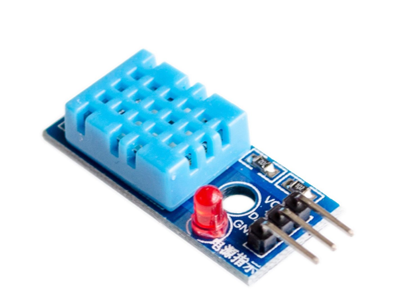
\includegraphics[scale = 0.5]{Sensor_temp_hum_dht11.png}
	\caption{Sensor de temperatura y humedad DHT11 \cite{tettsa_dht11}.}
	\label{fig:mesh11}
\end{figure}
\newpage
\subsection*{Módulo RTC (reloj de tiempo real)}
Los módulos RTC cuentan con un reloj interno el cual puede ser utilizado para determinar la hora y fecha con gran precisión. El módulo DS3231 cuenta con un protocolo de comunicación el cual permite conectar varios sensores en serie, reduciendo la cantidad de entradas y salidas requeridas en placas de desarrollo. A continuación se detallan las características del módulo \cite{la_electronica_DS3231}:

\begin{table}[H]
	\centering
	\begin{tabular}{|c|c|}
		\hline
		\multicolumn{2}{|c|}{\textbf{Placa del módulo RTC DS3231}}\\ \hline
		Voltaje de alimentación: & 3.3 a 5.5 VDC \\ \hline
		Precisión de reloj: & Error de 1 minuto a temperatura entre 0 y 40 °C \\ \hline
		Salida programable de onda cuadrada: & Sí \\ \hline
		Chip de memoria: & AT24C32 con capacidad de almacenamiento de 32kB \\ \hline
		Dimensiones: & 38 mm $\times$ 22 mm $\times$ 14 mm \\ \hline
		Peso: & 8g \\ \hline
	\end{tabular}
	\caption{Características de funcionamiento del módulo RTC DS3231.}
	\label{Cuadro:caracter_rtc}
\end{table}

\begin{figure}[H]
	\centering
	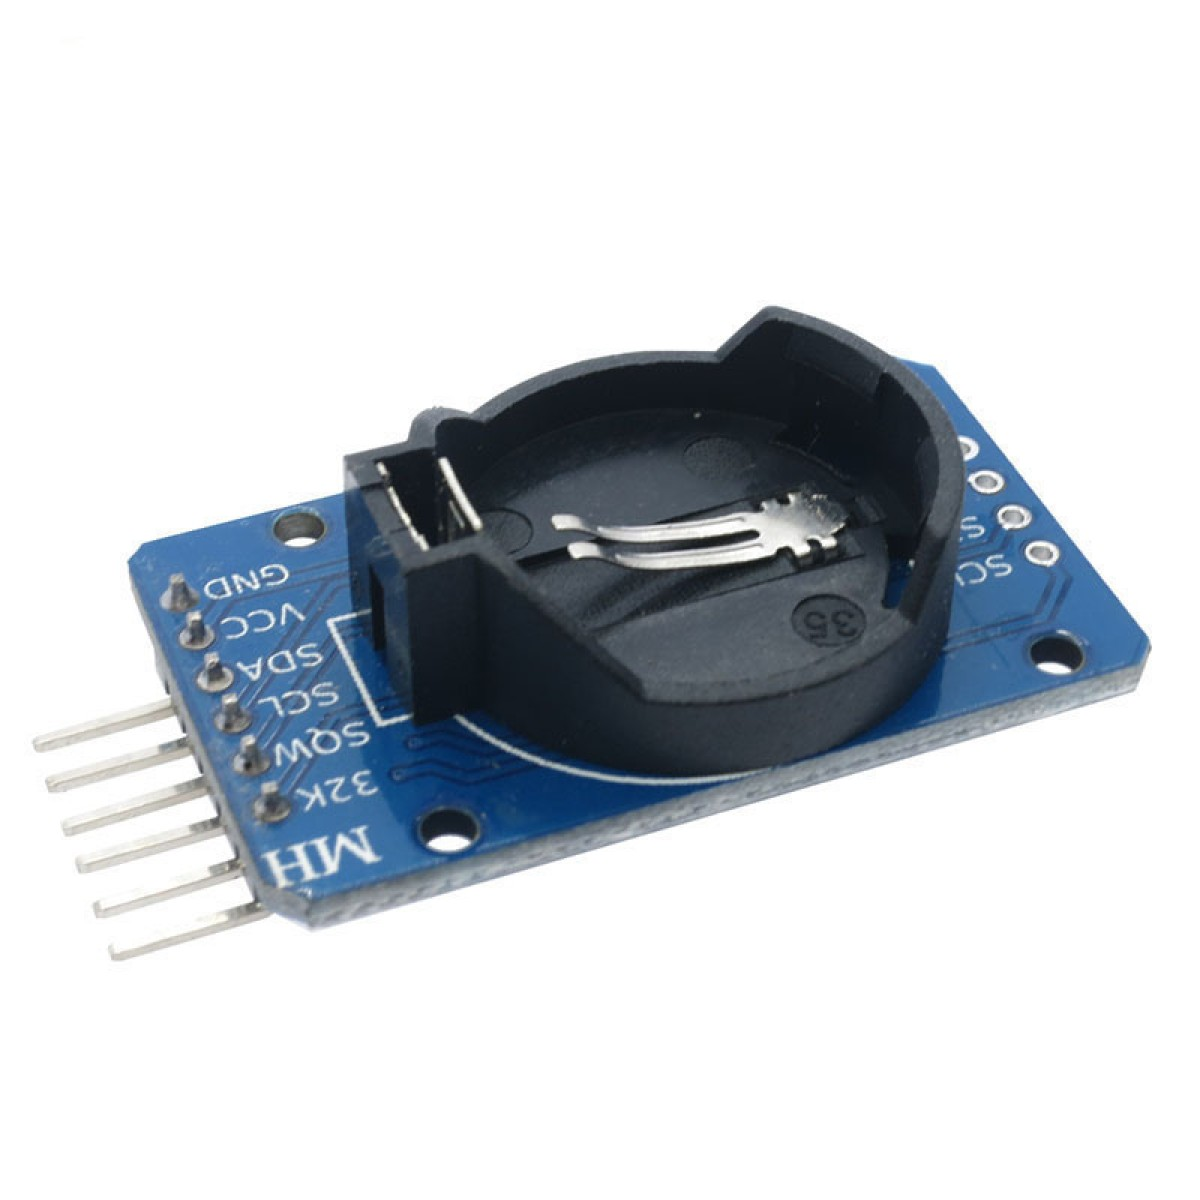
\includegraphics[scale = 0.15]{Figura_11_rtc.jpg}
	\caption{Módulo RTC DS3231 \cite{la_electronica_DS3231}.}
	\label{fig:modulo_rtc}
\end{figure}

\section{Placa de desarrollo \textit{ESP-WROOM-32}}
La ejecución de los procesos de control así como la recolección de datos de los sensores instalados requiere del uso de un microcontrolador. Las placas de desarrollo de la familia ESP32 son de gran utilidad, puesto que permiten la fácil integración del módulo ESP32 en cualquier proyecto. El módulo ESP32 es uno de los microcontroladores más versátiles y de menor costo disponibles en el mercado. Este cuenta con conectividad WiFi, \textit{Bluetooth} v4.2, \textit{Bluetooth Low Energy}, pines analógicos, diferentes protocolos de comunicación serial y paralela, dos núcleos de procesamiento y compatibilidad con el lenguaje de programación de Arduino. Adicionalmente, las placas de desarrollo diseñadas alrededor de este microcontrolador cuentan con un costo reducido y bajo consumo eléctrico, lo cual lo hace ideal para aplicaciones con limitantes de costos. A continuación se detallan las características generales de la placa de desarrollo \textit{ESP-WROOM-32} \cite{electronic_wings_espwroom32}:

\begin{table}[H]
	\centering
	\begin{tabular}{|c|c|}
		\hline
		\multicolumn{2}{|c|}{\textbf{Placa de desarrollo \textit{ESP-WROOM-32}}}\\ \hline
		Procesador: & 2 núcleos hasta 240 MHz \\ \hline
		WiFi: & 2.4 GHz hasta 150 Mbits/s \\ \hline
		\textit{Bluetooth}: & \textit{Bluetooth Low Energy} y \textit{Bluetooth} v4.2 \\ \hline
		Arquitectura del procesador: & 32 bits \\ \hline
		Memoria RAM: & 520 KB \\ \hline
		Cantidad de pines IO: & 38 \\ \hline
		Cantidad de pines tipo ADC: & 16 \\ \hline
		Botones disponibles: & Botón de arranque y reinicio \\ \hline
		Leds disponibles: & Indicador LED de estado \\ \hline
		Puente USB a UART: & CP2102 \\ \hline
	\end{tabular}
	\caption{Características de funcionamiento y conexión de la placa de desarrollo \textit{ESP-WROOM-32}.}
	\label{Cuadro6}
\end{table}

\begin{table}[H]
	\centering
	\begin{tabular}{|c|c|}
		\hline
		\multicolumn{2}{|c|}{\textbf{Periféricos adicionales}}\\ \hline
		\multicolumn{2}{|c|}{Sensor capacitivo integrado}\\ \hline
		\multicolumn{2}{|c|}{Conversor Digital Analógico}\\ \hline
		\multicolumn{2}{|c|}{I2C (\textit{Inter-Internal Circuit})}\\ \hline
		\multicolumn{2}{|c|}{UART (\textit{Universal asyncrhonous receiver/transmitter})}\\ \hline
		\multicolumn{2}{|c|}{SPI (\textit{Serial Peripheral Interface})}\\ \hline
		\multicolumn{2}{|c|}{PWM (\textit{Pulse Width Modulated})}\\ \hline
	\end{tabular}
	\caption{Protocolos de comunicación y otros periféricos disponibles en el \textit{ESP-WROOM-32}.}
	\label{Cuadro7}
\end{table}

\begin{figure}[H]
	\centering
	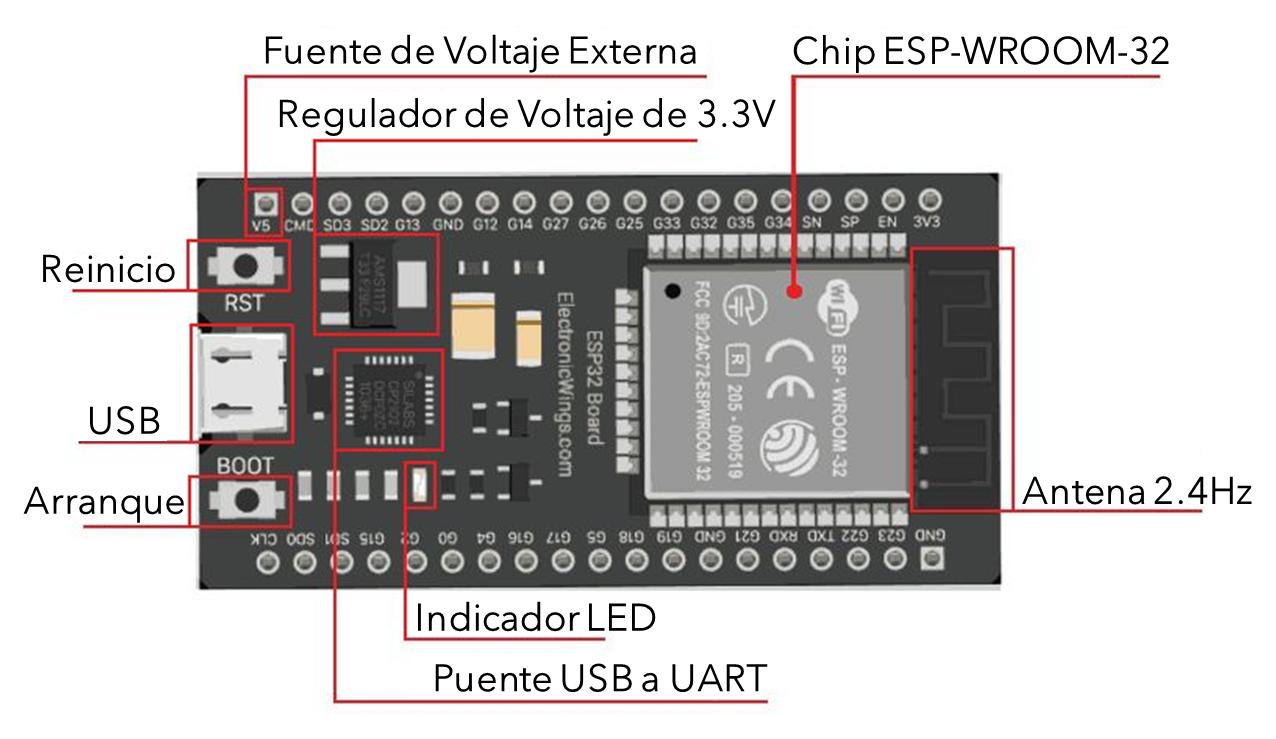
\includegraphics[scale = 0.5]{Figura_12_espwroom32.png}
	\caption{Componentes de la placa de desarrollo ESP-WROOM-32 \cite{electronic_wings_espwroom32}.}
	\label{fig:mesh12}
\end{figure}

\section{Sistemas de control y conectividad con la nube}

\subsection{El internet de las cosas (IoT)}
El internet de las cosas se refiere a la capacidad de conectar objetos de uso cotidiano al internet para compartir parámetros de funcionamiento y otros datos entre diferentes dispositivos. La capacidad de compartir datos de manera inalámbrica con poca intervención humana hace de este proceso ideal para la automatización de procesos en diferentes sectores, desde el hogar hasta la ciudad entera. En general, los dispositivos IoT se pueden categorizar en sensores y actuadores o controladores, donde estos cumplen la función de recolectar datos y activar procesos respectivamente. Un sistema IoT básico funciona mediante un ciclo de retroalimentación constante de recolección, envío y análisis de datos para controlar diferentes eventos o indicar el estado de estos. El internet de las cosas se puede encontrar en una gran variedad de aplicaciones, desde la industria de manufactura, procesos de logística y transportación de productos hasta la agricultura. \cite{redhat_IoT_2019}

\begin{figure}[H]
	\centering
	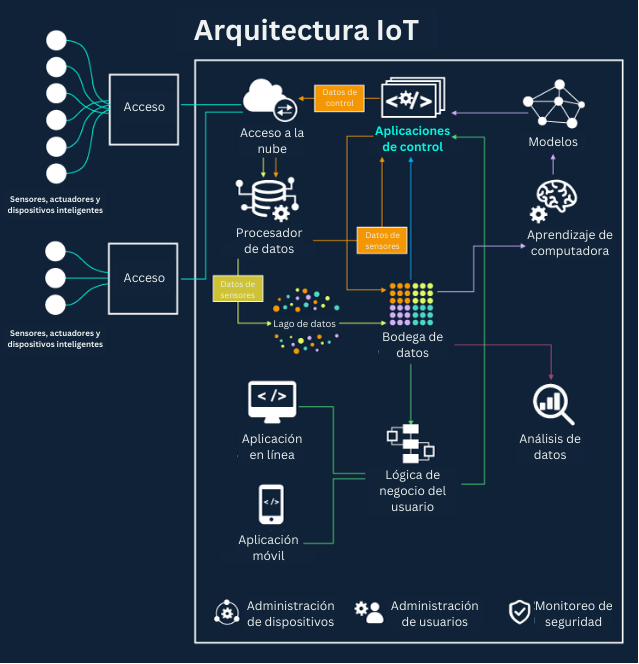
\includegraphics[scale = 0.55]{Figura_13_arquitectura_iot.png}
	\caption{Diagrama de la arquitectura IoT generalizada \cite{grizhnevich_iot_2018}.}
	\label{fig:mesh13}
\end{figure}

\subsection{Protocolo de comunicación HTTP}
El internet funciona gracias a una serie de protocolos de comunicación que permiten la transferencia de datos como imágenes, texto, videos y audios entre servidores y usuarios. Uno de los protocolos fundamentales para la transmisión de estos datos es el protocolo HTTP (\textit{Hypertext Transfer Protocol}) o Protocolo de Transferencia de Hipertexto. La primera versión de HTTP para la transferencia de datos fue utilizada en 1990 como una herramienta para enviar datos a un usuario. Esta primera versión se conoce como HTTP/0.9. Esta iteración del protocolo se conoció como el protocolo de una línea, puesto que contaba con una gran cantidad de limitaciones, permitiendo únicamente realizar búsquedas de elementos como páginas escritas en HTML, imágenes o archivos específicos \cite{Evolution_http_Mozilla_2024}. Unos años después, gracias a un esfuerzo conjunto entre el MIT, \textit{Microsoft} y otras empresas, se desarrolló el protocolo HTTP/1.1. Una de las ventajas principales de este nuevo protocolo consistía en la adición de sistemas para el envío de datos a un servidor. Adicionalmente, se definieron nuevas reglas que permitieron que este sistema fuese más estable e incluso permitiera la transferencia de datos de manera simultánea \cite{fielding_hypertext_1999}. Este protocolo estableció los fundamentos para el desarrollo de futuras versiones, actualmente, las más utilizadas son  es la versión HTTP/2.0 y HTTP/3.0.

El protocolo HTTP consiste en el uso de una solicitud con una instrucción específica la cual es transmitida desde un usuario o cliente (\textit{client}). Esta solicitud se realiza mediante una conexión TCP o UDP dependiendo de la versión del protocolo, y cuenta con una estructura estandarizada para extraer, agregar, cambiar o eliminar información en el servidor. Una solicitud para retirar datos presenta la estructura observada en la Figura \ref{fig:mesh14}. Las palabras \textit{GET}, \textit{POST}, \textit{PUT}, \textit{PATCH} y \textit{DELETE} son utilizadas para indicarle al servidor durante la solicitud realizada las acciones a realizar. Adicionalmente, se especifica la dirección del servidor junto con información importante para la transacción y el contenido del mensaje en caso de que este sea requerido \cite{overview_http_mozilla_2024}.

\begin{figure}[H]
	\centering
	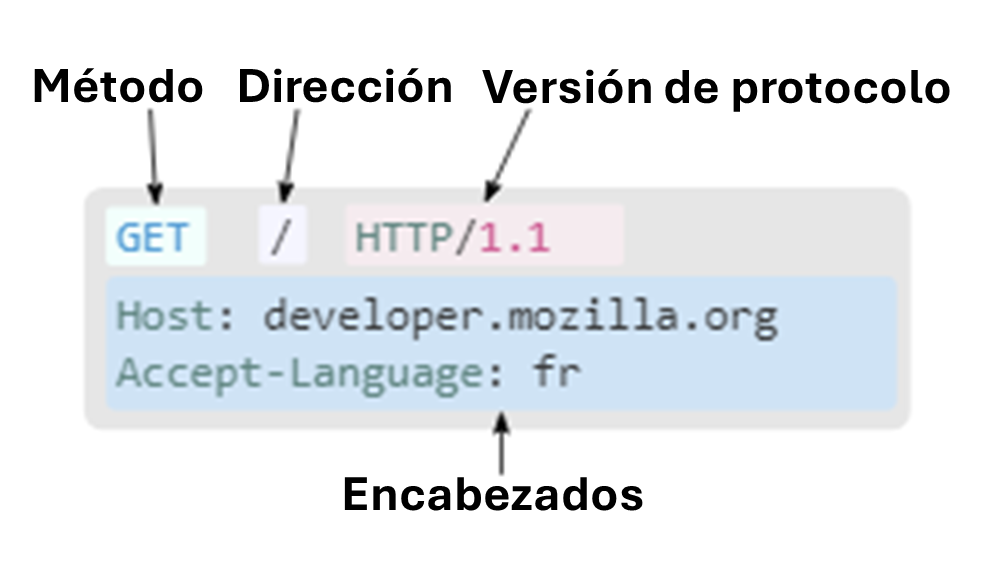
\includegraphics[scale = 0.35]{Figura_14_solicitud_http.png}
	\caption{Estructura de una solicitud para retirar datos en el protocolo HTTP/1.1 \cite{overview_http_mozilla_2024}.}
	\label{fig:mesh14}
\end{figure}

Las solicitudes realizadas por el cliente son dirigidas directamente al servidor indicado en la dirección, sin embargo, usualmente se utilizan dispositivos intermedio para realizar dicha conexión. Una vez que el servidor recibe la solicitud, este devuelve una respuesta con un encabezado en el cual se detallan las características del archivo, así como ciertos códigos para indicar el estado de la conexión. Adicionalmente, la respuesta del servidor contará con la información solicitada por el cliente, ya sea esta un segmento de texto, un archivo, una página web o un video. Gracias a su simplicidad, este protocolo es el más utilizado hoy en día para intercambios de información en la red \cite{overview_http_mozilla_2024}.

\begin{figure}[H]
	\centering
	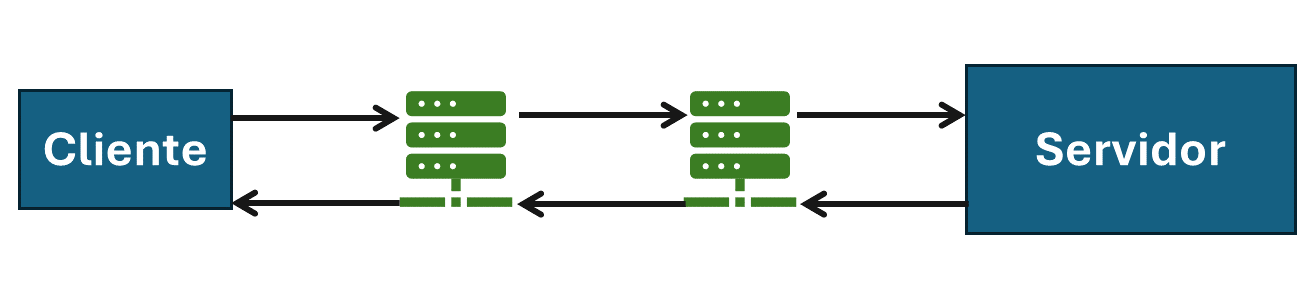
\includegraphics[scale = 0.4]{Figura_14.1_comunicacion_http.png}
	\caption{Diagrama de la comunicación entre cliente y servidor mediante el protocolo HTTP \cite{overview_http_mozilla_2024}.}
	\label{fig:mesh14_1}
\end{figure}

\subsection{Comunicación WiFi con \textit{Dweet.io}}
\textit{Dweet.io} es un servicio abierto al público y totalmente gratuito que permite la transferencia de datos entre dispositivos funcionando como servidor para comunicaciones mediante HTTP. \textit{Dweet.io} utiliza un tema, llamado \textit{Thing}, el cual funciona como un servidor que recibe solicitudes mediante HTTP. Esta funcionalidad permite que diferentes dispositivos con conexión a la red puedan solicitar información almacenada o cargar nuevos datos a este servidor utilizando la dirección del tema. Una de sus mayores ventajas es que almacena datos en la forma de texto, el cual es distribuido en el cuerpo de las solicitudes HTTP. Esto permite almacenar diferentes valores de manera legible para cualquier humano, facilitando así el proceso de recolección e intercambio de datos. Es importante destacar que al ser gratuito, este servicio es completamente público y los mensajes pueden ser leídos por cualquiera con acceso a este servicio \cite{dweet_dweetio_faq}. Adicionalmente, los mensajes enviados a los servidores de \textit{Dweet.io} son almacenados únicamente durante 24 horas, a menos de que se pague una suscripción a un servidor privado.

\begin{figure}[H]
	\centering
	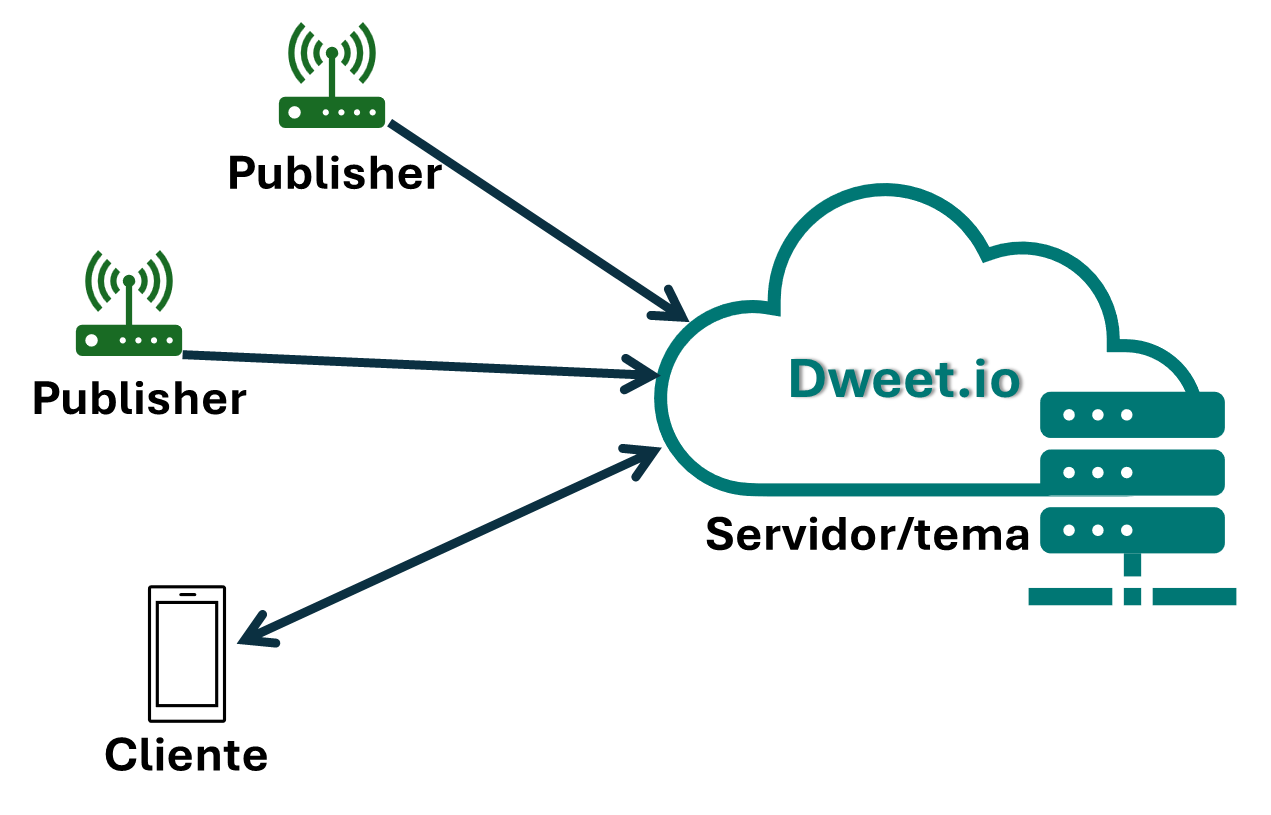
\includegraphics[scale = 0.4]{Figura_16_comunicacion_dweetIO.png}
	\caption{Diagrama de la comunicación entre cliente y servidor de \textit{Dweet.io}.}
	\label{fig:mesh16}
\end{figure}

\subsection{Controladores de Fuzzy Logic}
En el área de control de sistemas, existen casos en donde el sistema a controlar presenta una gran cantidad de entradas y salidas así como una alta complejidad matemática en las variables de estado que lo definen, en la forma de no linealidades. En estos casos, el desarrollo de un modelo matemático que sea capaz de describir adecuadamente todas las relaciones entre variables llega a ser demasiado complejo, por lo cual se buscan alternativas para el control. Uno de los métodos diseñados para el control de estos sistemas se basa en la teoría de \textit{Fuzzy Sets} el cual busca establecer rangos de funcionamiento lineales para las variables de control del sistema así como relaciones lineales entre los diferentes parámetros que estas controlan. Estos se logra mediante procesos matemáticos para obtener rangos que permitan un control adecuado del sistema, sin la realización de un modelo matemático que describa todas las dinámicas del sistema \cite{verbruggen_fuzzy_1999}.




	\fi
\fi

% CAPÍTULOS
% ------------------------------------------------------------------------------
\newpage
\ifdefined\parpordefecto
	\defaultparformat{j-capitulos}
\else
	
%----------------------------------------------------------------------------------------------------------

\chapter{Diseño y ensamblaje del sistema hidropónico}

En el presente capítulo se detallan los procesos, metodologías, retos y soluciones encontradas durante el desarrollo de la estructura física del sistema hidropónico. Este proceso de desarrollo se puede segmentar en tres etapas esenciales: diseño de estructura, diseño de circuitos y la construcción del sistema. A lo largo de estas etapas se encontraron retos y dificultades, así como oportunidades de mejora luego de las pruebas de funcionamiento realizadas.

\section{Diseño de la estructura}

El proceso de diseño atravesó diferentes etapas de iteración, en las cuales se encontraron áreas de mejora que facilitaran el proceso de manufactura y adquisición de la estructura. Durante las etapas iniciales, se propuso una iteración la cual se centraba en un proceso de manufactura extenso, utilizando como base perfiles angulares de aluminio 6061-T6. Si bien este diseño de la estructura cumplía con algunos de los requerimientos, se determinó que el proceso de manufactura sería un factor considerable, por lo que se diseñó una nueva iteración utilizando una estructura base prefabricada. A continuación se detallan las iteraciones diseñadas así como las consideraciones generales que llevaron a la elección de la última iteración para su construcción.

\subsection{Requerimientos físicos y restricciones de espacio}

La estructura física del sistema funcionaría como la plataforma que integraría todos los componentes necesarios para el funcionamiento del sistema hidropónico automático. Entre estos, se resaltan el depósito de almacenamiento de solución nutritiva, los canales de crecimiento, las tuberías de distribución de agua, los diferentes sensores, ventiladores, luces de crecimiento y actuadores, así como el sistema de control y la fuente de potencia. Esto, junto con las restricciones de espacio establecidas en los objetivos específicos del presente trabajo de graduación, establecieron requerimientos críticos relacionados a la estructura del sistema los cuales se detallan a continuación:

\begin{itemize}
	\item Altura máxima aproximada de 1750 mm para acomodar espacio entre repisas de aproximadamente 400 mm.
	\item Ancho de repisas de 700 mm para acomodar plantas con un espacio de 180 mm entre sí.
	\item Adaptabilidad para instalar sensores, actuadores y demás elementos necesarios para el funcionamiento del sistema, tanto antes como después del ensamblaje de la estructura principal.
	\item Rigidez estructural para soportar el peso del agua circulando por el sistema.
	\item Resistencia a la corrosión debido a exposición a altos niveles de humedad.
	\item Repisas de madera o plástico rígidas que permitan realizar modificaciones como agujeros o ranuras para ventilación y fijación de componentes.
	\item Facilidad de construcción con un proceso de manufactura sencillo sin el uso de herramientas altamente especializadas.
\end{itemize}

\subsection{Primera iteración, estructura de aluminio}

Como se mencionó al inicio de esta sección, la primera iteración de la estructura principal se diseñó utilizando perfiles estándar de dos pulgadas de aluminio 6061-T6. Se seleccionó este material considerando su facilidad de corte, baja densidad y alta disponibilidad en el país. Adicionalmente, se consideró que esta aleación es resistente a la corrosión y admite fácilmente la aplicación de recubrimientos tanto estéticos como funcionales \cite{matweb_al6061_T6}. 

Como se observa en la Figura \ref{fig:alumin}, la estructura se diseñó utilizando cuatro perfiles verticales, unidos por una serie de perfiles horizontales para las repisas a distancias preestablecidas. Una de las primeras limitaciones observadas durante las etapas de evaluación de este diseño fueron los altos requerimientos de maquinado para su manufactura. Según el diseño elaborado, esta iteración requería agujeros y cortes precisos, los cuales serían necesarios para instalar tornillos de fijación y tuberías de distribución.

\begin{figure}[H]
	\centering
	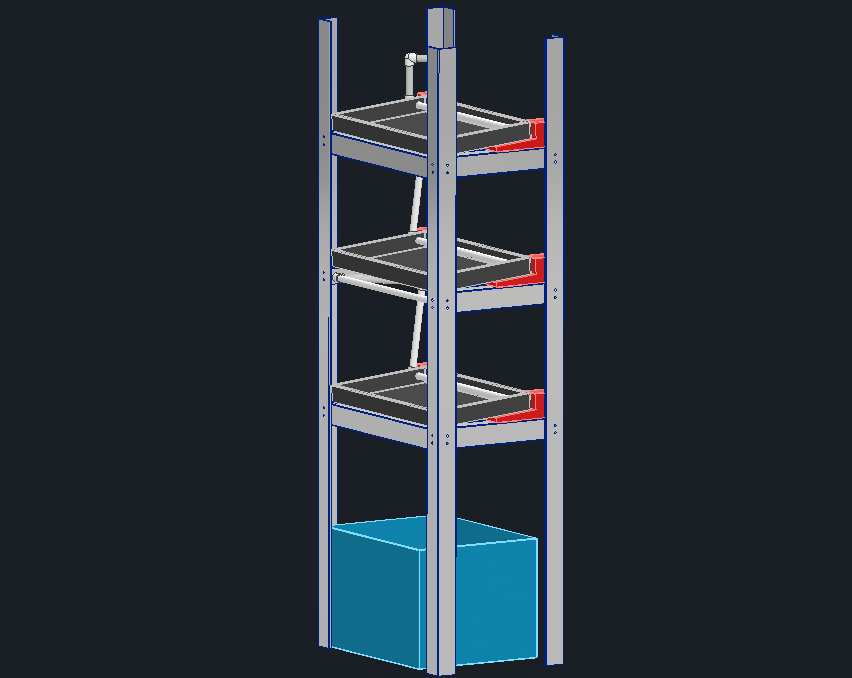
\includegraphics[scale= 0.4]{Figura_17_primera_iteracion_estructura.png}
	\caption{Estructura inicial diseñada utilizando perfiles de aluminio de dos pulgadas.}
	\label{fig:alumin}
\end{figure}

Una vez completado el modelo CAD del sistema, se analizaron los requerimientos de manufactura. Si bien se eliminó la necesidad de realizar soldaduras en aluminio para unir los diferentes perfiles. Esta decisión de diseño implicó agregar una mayor cantidad de agujeros para elementos de fijación mecánicos. Por esta razón, el proceso de fabricación requeriría tanto del corte de los perfiles, utilizando cierra de calar u otras herramientas de corte afines, como el taladrado de agujeros. Adicionalmente, varios de los perfiles, como se observa en la Figura \ref{fig:perfil_h}, contaban con agujeros de diámetros mayores para tuberías, los cuales deberían ser maquinados en una máquina fresadora. Considerando los diferentes procesos de maquinado, se determinó que esta etapa de construcción requeriría de una inversión de tiempo considerable.

\begin{figure}[H]
	\centering
	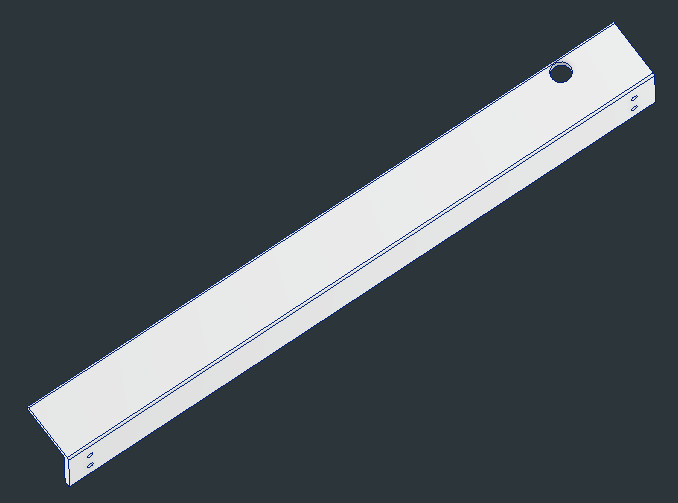
\includegraphics[scale= 0.6]{Perfil_horizontal_aluminio.png}
	\caption{Perfil horizontal con perforación para tubería de distribución.}
	\label{fig:perfil_h}
\end{figure}
\newpage
\subsubsection{Canales de crecimiento}

Como se observa en la Figura \ref{fig:alumin}, en esta iteración se contempló el uso de bandejas de forraje las cuales permitirían el flujo del agua sobre su superficie, logrando así el suministro de nutrientes a las plantas. Adicionalmente, se utilizaron tuberías de PVC de 0.5 pulg, las cuales estarían a cargo de distribuir la solución nutritiva hacia las bandejas de crecimiento y entre cada nivel del sistema. Al utilizar tuberías de distribución para la solución nutritiva, se diseñaron perforaciones que serían necesarias en las bandejas de crecimiento para integrarlas con las tuberías. Adicionalmente, sería necesario implementar una cobertura para las bandejas de crecimiento, que mantuviera oscuro el entorno de las raíces, mientras que brindan una estructura de fijación para las plantas.

\begin{figure}[H]
	\centering
	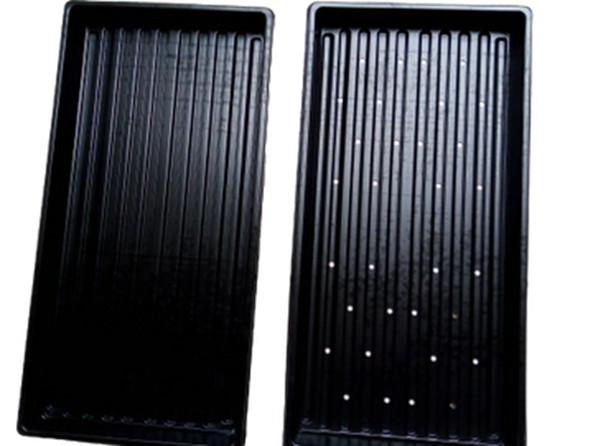
\includegraphics[scale= 0.6]{Bandeja_forraje.png}
	\caption{Bandejas de forraje a utilizarse como canales de crecimiento.}
	\label{fig:bandeja_forraje}
\end{figure}

Una de las ventajas identificadas en las bandejas de forraje fue su versatilidad a la hora de distribuir las plantas. Sin embargo, se observó que las bandejas disponibles en el mercado guatemalteco, ver la Figura \ref{fig:bandeja_forraje}, contaban con canales que limitaban demasiado el flujo de agua, y podrían llevar a puntos secos. Estas áreas sin agua se deben a la irregularidad en el flujo del agua a través de la superficie de las bandejas, lo cual presentaría un riesgo significativo hacia las plantas. Adicionalmente, durante las etapas de diseño se determinó que la cantidad de material necesaria para cubrir las bandejas de crecimiento sería significativa. Estos cobertores para las bandejas requerirían de procesos de impresión por partes, lo cual dificultaría el proceso de construcción. Finalmente, las modificaciones necesarias para asegurar un flujo de agua constante entre las repisas generaría puntos de fuga los cuales podrían llegar a presentar un riesgo para el sistema. Por estas razones, se decidió iniciar una nueva iteración para el diseño del sistema.

\subsection{Segunda iteración, estructura prefabricada}

Si bien la primera iteración permitía una mayor flexibilidad en cuanto al diseño de la estructura, el proceso de fabricación dificultaba cualquier modificación que llegara a ser necesaria. Adicionalmente, al utilizar perfiles de aluminio, esta primera iteración requeriría de una gran cantidad de perfiles de aluminio, los cuales serían difíciles de transportar e instalar. Por esta razón, se inició una segunda iteración buscando utilizar una estructura prefabricada, la cual se pudiera adecuar de manera que fuera funcional en el sistema sin grandes modificaciones.

Luego de unas búsquedas en internet, se encontró una estantería de 1520 mm de altura y 760 mm de ancho. Adicionalmente, contaba con repisas de madera MDF con marcos de metal, las cuales podían ser instaladas a diferentes alturas. Como se observa en la Figura \ref{fig:estanteria_prefab}, se creó un modelo 3D de la estantería, con el cual fue posible observar los beneficios de esta selección en el diseño. Algunas de las ventajas incluyen a las estanterías de madera, las cuales se pueden modificar con facilidad y permiten el uso de tornillos de madera para la fijación de diferentes componentes. Así mismo, los perfiles con ranuras de ojo de cerradura, Figura \ref{fig:Perfil_slotted} se pueden aprovechar para instalar diferentes componentes en el sistema utilizando tornillos y tuercas sin la necesidad de modificar la estructura física. 

\begin{figure}[H]
	\centering
	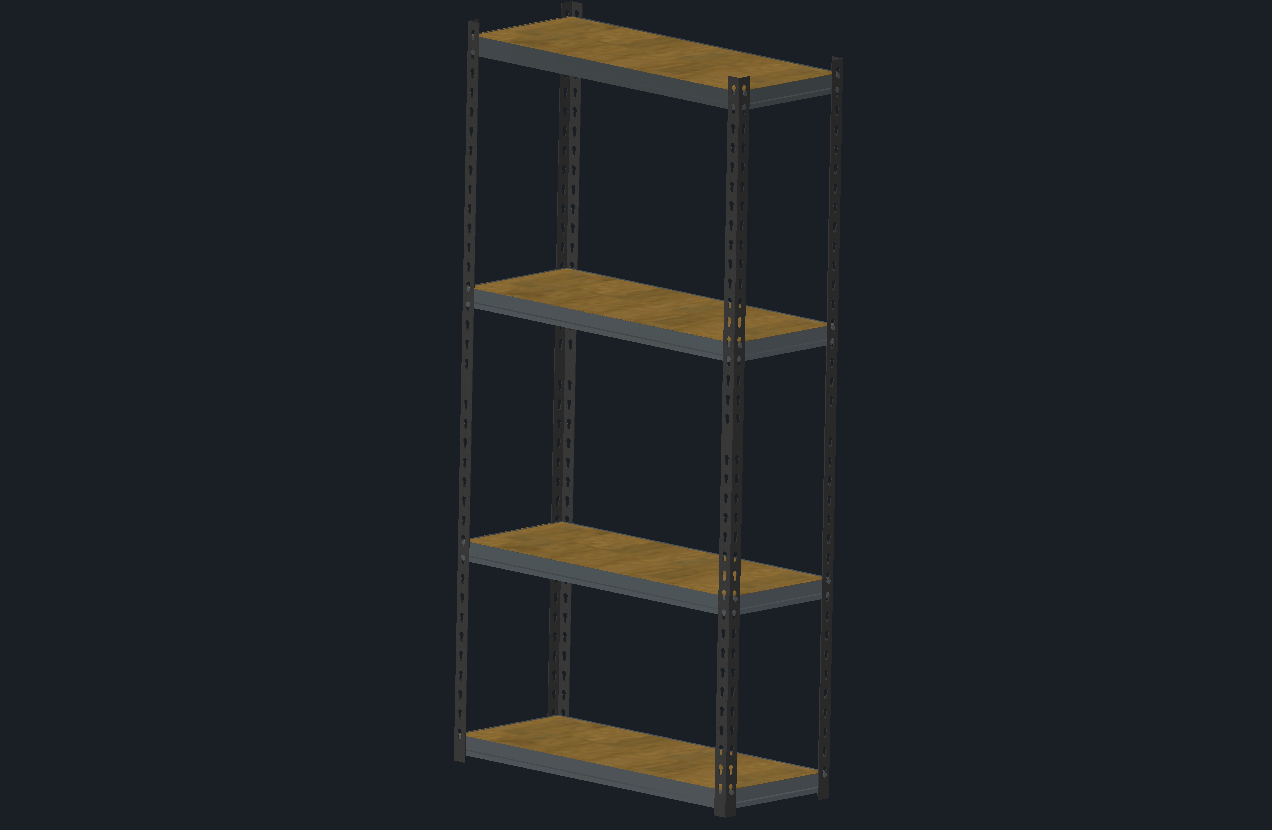
\includegraphics[scale= 0.35]{Estanteria_prefabricada.png}
	\caption{Modelo 3D de la estantería prefabricada.}
	\label{fig:estanteria_prefab}
\end{figure}

\begin{figure}[H]
	\centering
	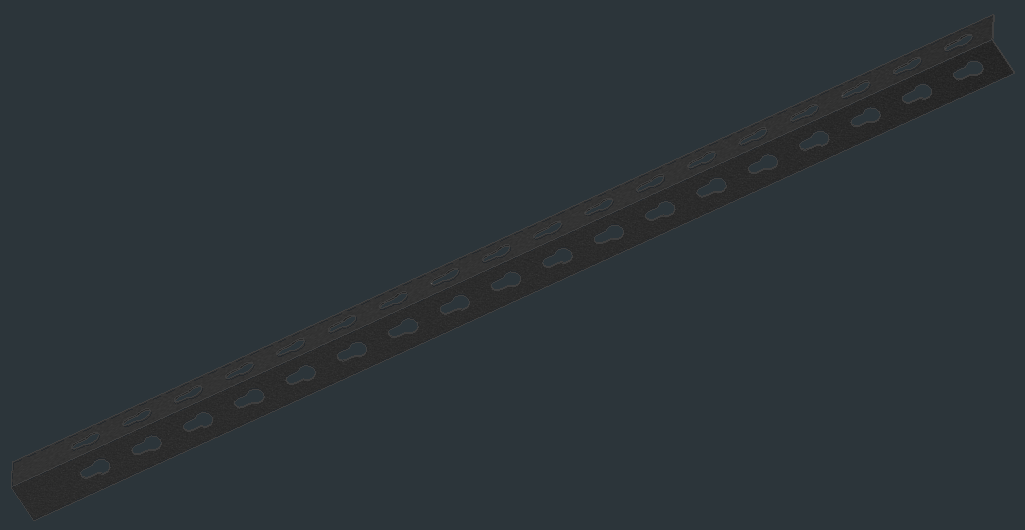
\includegraphics[scale= 0.4]{Perfil_slotted_1.png}
	\caption{Perfil con ranuras de ojo de cerradura.}
	\label{fig:Perfil_slotted}
\end{figure}

\subsubsection{Canales de crecimiento}

Una vez se había definido la estructura de soporte del sistema en la segunda iteración, se continuó con el diseño del sistema de distribución de nutrientes. Con tal de mejorar la canalización del agua y asegurar que las raíces de las plantas recibieran una cantidad adecuada de agua, se seleccionaron tuberías de PVC para los canales de crecimiento de las plantas. Estas tuberías, además de asegurar que el agua se desplazara por una ruta predecible y predeterminada, facilitaban el proceso de construcción. Adicionalmente, estas tuberías de PVC se encontraban con facilidad en el mercado guatemalteco, y no requerían de grandes esfuerzos para su ensamblaje. Por otro lado, el uso de estas tuberías elimina la necesidad de encontrar una forma cubrir los canales de crecimiento, puesto que únicamente es necesario crear agujeros puntuales en la tubería para el crecimiento de las plantas. 

Al tomar en cuenta las consideraciones anteriores, se seleccionaron tuberías de 2.5 pulg, las cuales, junto con uniones de codo a 90° y uniones tipo T, permitirían la elaboración de los canales de crecimiento del sistema. Si bien la mayoría de las modificaciones necesarias para las tuberías consistirían en cortes, agregaron perforaciones de 2 pulg de diámetro las cuales permitirían introducir las canastas de crecimiento en las tuberías. Finalmente, se definió una orientación longitudinal para los canales de crecimiento, la cual permitiría instalar dos tiras de luces de crecimientocon una longitud aproximada de 500 mm en cada nivel. 

\begin{figure}[H]
	\centering
	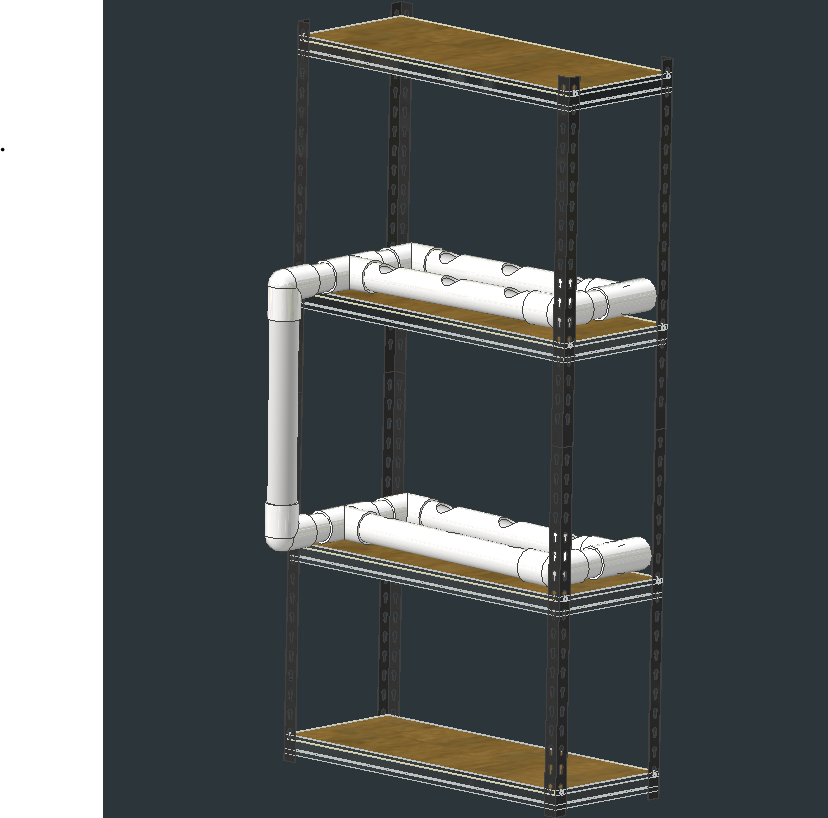
\includegraphics[scale= 0.4]{Canales_crecimiento_estructura.png}
	\caption{Estructura con canales de crecimiento.}
	\label{fig:canales_crecimiento}
\end{figure}

Como se observa en la figura anterior, los canales de distribución de solución nutritiva y de crecimiento, se diseñaron completamente utilizando tuberías y accesorios de PVC. Esta decisión de diseño simplificó considerablemente su ensamblaje mientras que aseguraba un flujo adecuado para las plantas. Si bien las tuberías serían capaces de transportar el agua sin dificultad, aún sería necesaria una inclinación para asegurar el flujo constante de agua. Domando en cuenta la curvatura de las tuberías, se diseñaron dos soportes los cuales permitirían crear tanto una inclinación longitudinal como transversal. Estas inclinaciones serían necesarias para promover el flujo del agua desde el nivel superior hasta el inferior, y a través de las tuberías de crecimiento. Como se observa en la Figura \ref{fig:soporte_tub}, los soportes consistirían de piezas rectangulares con una sección semicircular inclinada a un ángulo de 0.8°, lo cual brindaría la pendiente necesaria para el flujo de agua requerido por el sistema. Estos soportes serían impresos en 3D para facilitar su manufactura, y se utilizarían tornillos para fijarlos a las superficies de las repisas. Cabe mencionar que se crearon dos soportes idénticos de alturas diferentes con tal de obtener una inclinación transversal entre las tuberías y asegurar así el flujo entre niveles.

\begin{figure}[H]
	\centering
	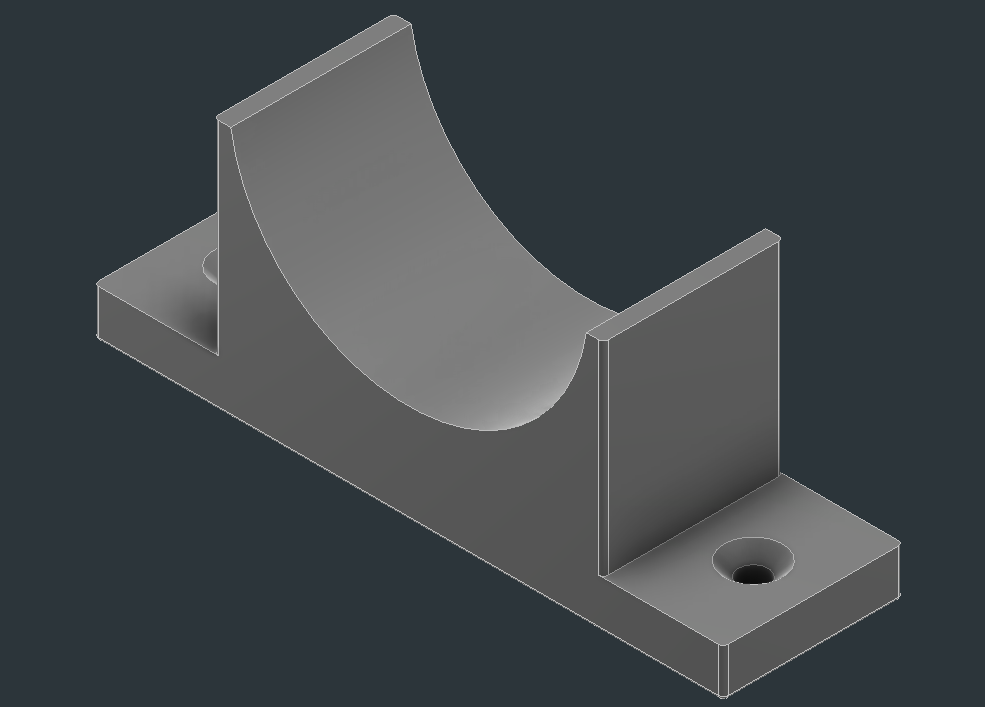
\includegraphics[scale= 0.4]{Soporte_tuberias.png}
	\caption{Soporte con inclinación de 0.8° para tuberías de crecimiento.}
	\label{fig:soporte_tub}
\end{figure}

\subsection{Comparación de las iteraciones de diseño de la estructura}

Si bien la segunda iteración del diseño presentó grande mejoras en cuanto a la facilidad de ensamblaje y construcción, se realizó una comparación entre ambas iteraciones para determinar cuál sería utilizada en el sistema final. A continuación, se encuentra un cuadro comparativo en donde se evaluaron ambas iteraciones respecto a los requerimientos establecidos en la sección 7.1.1. del presente capítulo.

\begin{table}[H]
	\centering
	\begin{tabular}{|c|c|c|} \hline
		~ & \textbf{Primera iteración} & \textbf{Segunda iteración}\\ \hline
		\textbf{Altura max.} & 1750 mm & 1520 mm  \\ \hline
		\textbf{Ancho de repisas} & 586.7 mm & 760 mm \\ \hline
		\textbf{Adaptabilidad} & Pre construcción & Pre y post construcción \\ \hline
		\textbf{Rigidez estructural} & Media & Alta \\ \hline
		\textbf{Resistencia a la corrosión} & Alta & Media \\ \hline
		\textbf{Repisas de madera} & Sin repisas de madera & Repisas de MDF \\ \hline
		\textbf{Facilidad de construcción} & Manufactura compleja & Ensamblaje rápido \\ \hline
	\end{tabular}
	\caption{Análisis comparativo entre primera y segunda iteración de la estructura.}
	\label{cuadro:compar_iter}
\end{table}

Luego de analizar las características del diseño desarrollado para ambas iteraciones como se observa en el Cuadro \ref{cuadro:compar_iter}, se determinó que la segunda iteración sería la más factible para su desarrollo. Esto debido a que cumplió de mejor manera con los requisitos de facilidad de construcción, adaptabilidad \footnote{Esta se ponderó en función de la facilidad de realizar modificaciones una vez se haya instalado el sistema.} y rigidez estructural \footnote{Se determinó que la rigidez estructural de la primera iteración sería menor debido a una mayor altura y menor ancho de repisas, lo cual haría de la estructura menos estable}. Una vez se determinó estructura a utilizar, se iniciaron los procesos de diseño secundarios.

\subsection{Diseño de componentes auxiliares}

Luego del proceso de diseño de la estructura principal, se inició el diseño de los componentes que permitirían integrar la estructura principal con los sensores y actuadores requeridos. Con tal de facilitar el proceso de manufactura, se definieron las siguientes restricciones y consideraciones. Estas deberían ser cumplidas con todos los diseños realizados, asegurando un ensamblaje sencillo.

\begin{itemize}
	\item Simplicidad para impresión 3D: Para modelos pequeños, que su diseño cuente con chaflanes, redondeados y ángulos adecuados con tal de facilitar su manufactura utilizando impresoras 3D con materiales como PLA, ABS o PETG.
	\item Factibilidad de manufactura utilizando corte láser: En caso de que el modelo sea demasiado grande, que este pueda ser fabricado utilizando corte láser con materiales como MDF o acrílico.
	\item Facilidad de ensamble: Que los modelos se puedan ensamblar fácilmente utilizando tornillos u otros medios mecánicos.
\end{itemize}

Utilizando las consideraciones anteriores, se diseñaron dos componentes secundarios. En la Figura \ref{fig:soporte_dht} se observa el primer componente, utilizado para fijar los sensores de temperatura y humedad DHT11 a las repisas de crecimiento. Estos sujetadores para los sensores de DHT11 deberían permitir que se instalaran a una distancia cercana a la altura de las plantas. Esto para asegurar que los parámetros recolectados fueran representativos del entorno alrededor de las hojas y tallos en cada repisa. Para esto se definió el uso de una varilla de madera de 0.5 pulg de diámetro, la cual sería cortada a una longitud aproximada de 160 mm. Los sensores se acoplaron a un anillo, el cual sería fijado a las varillas mediante un tornillo para madera.

\begin{figure}[H]
	\centering
	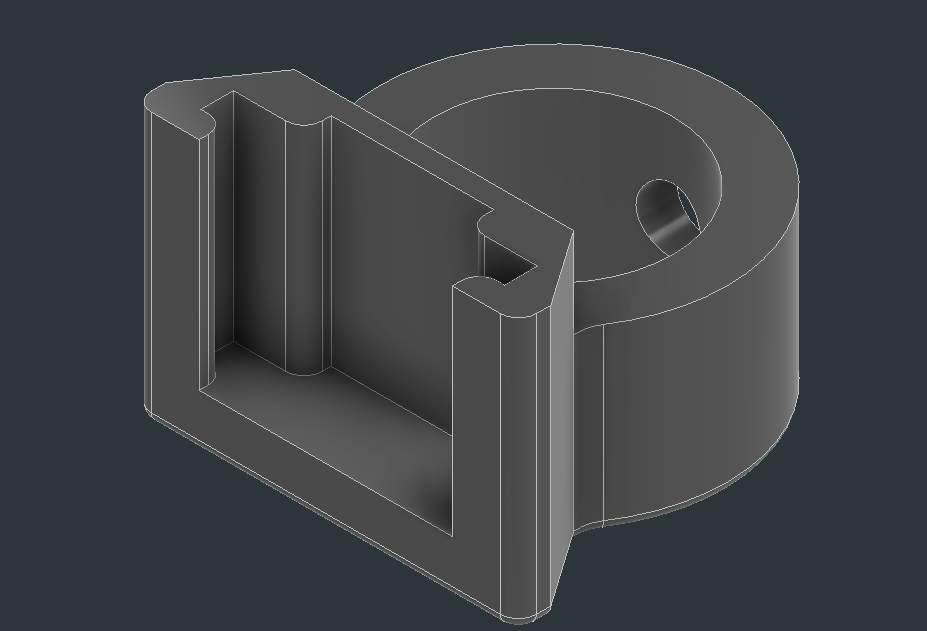
\includegraphics[scale= 0.4]{Soporte_dht11.png}
	\caption{Soporte para sensores DHT11 en varillas de 0.5 pulg.}
	\label{fig:soporte_dht}
\end{figure}

En el caso del segundo componente, este se diseñó para fijar los ventiladores a la estructura de metal. Se diseñaron considerando los agujeros disponibles en cada ventilador para su instalación. Adicionalmente, se diseñó un agujero central que permitiría el uso de tornillos para fijar mecánicamente el soporte a los postes de metal, aprovechando las ranuras de ojo de cerradura. Como se observa en la Figura \ref{fig:soporte_vent}, este componente presenta una baja complejidad, facilitando el proceso de manufactura e instalación.

\begin{figure}[H]
	\centering
	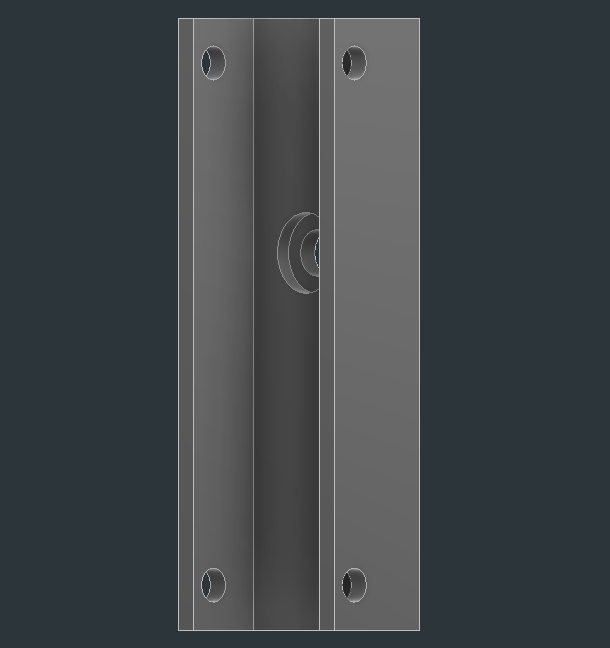
\includegraphics[scale= 0.4]{Soporte_ventilador.png}
	\caption{Soporte para ventiladores con tornillos de 0.25 pulg.}
	\label{fig:soporte_vent}
\end{figure}

\subsection{Modelado CAD de la estructura}

Una vez finalizados los diferentes modelos a instalar en el diseño de la segunda iteración, se integraron todos los componentes para tener un modelo completo del sistema. Como se observa en la Figura \ref{fig:estanteria_v2}, este modelo cuenta con las tuberías de distribución, canales de crecimiento, tanque de almacenamiento de agua. Además, cuenta con las varillas para la sujeción de los sensores y demás componentes auxiliares.

\begin{figure}[H]
	\centering
	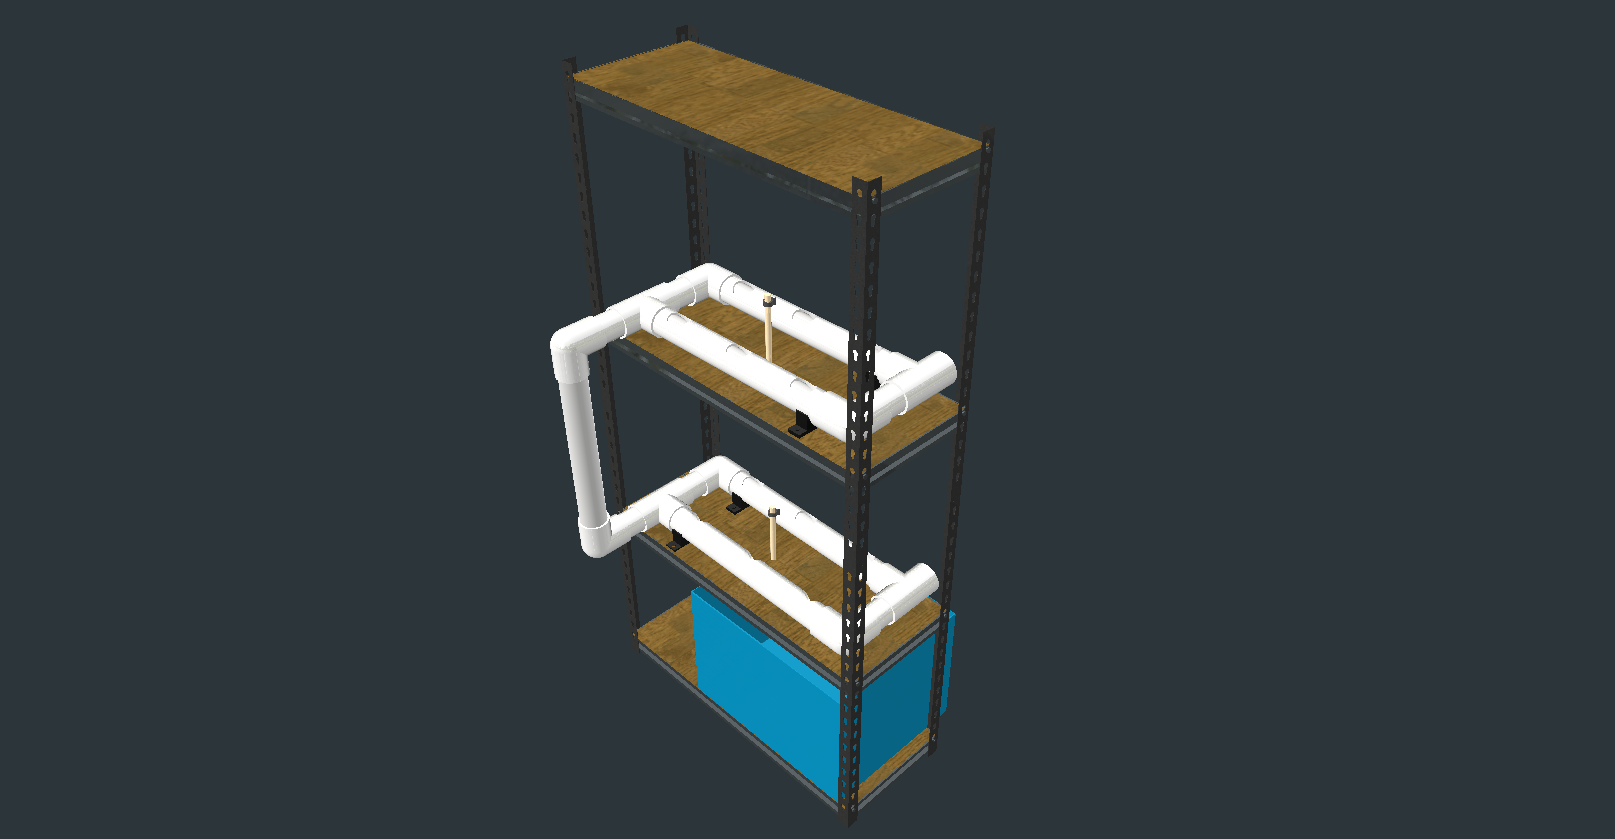
\includegraphics[scale= 0.4]{TH_ensamble_prototipo_v2.png}
	\caption{Ensamblaje del modelo CAD de la estructura principal del sistema.}
	\label{fig:estanteria_v2}
\end{figure}

Con este modelo establecido, fue posible continuar con el proceso de construcción, el cual se discutirá en la sección 7.3. del presente capítulo.

\section{Diseño de circuitos}

El sistema de control se basó en el microcontrolador ESP-WROOM32 y la placa de desarrollo de \textit{Hiletgo} ESP-32S. Esta placa se utilizó para obtener información de los diferentes sensores y activar los actuadores conectados al sistema. Debido al uso de un microcontrolador con una placa de desarrollo, la mayor parte de los circuitos del sistema se categorizaron como conexiones de componentes digitales. Si bien esto redujo la complejidad del proceso en el diseño de los circuitos, se encontraron varios retos relacionados a niveles de voltaje y disponibilidad de conexiones en la placa de desarrollo. A continuación, se detallan las diferentes etapas consideradas en el diseño del sistema electrónico.

\subsection{Características de alimentación de potencia}

Desde el controlador hasta los sensores, luces y actuadores requieren de una alimentación regulada de voltaje CC (corriente continua). Como se discutió en el capítulo 6, la mayoría de los componentes utilizados cuentan con un rango de voltaje de operación entre los 3 y 5.5 voltios CC. Por otro lado, los ventiladores a utilizar en el sistema consistirían de ventiladores de corriente alterna, por lo que sería necesario acceso a una línea de 120 voltios CA (corriente alterna). Por estas razones, la fuente seleccionada debería ser capaz de entregar un voltaje de 5 voltios CC y ser capaz de funcionar con una entrada de 120 voltios CA. Adicionalmente, en el capítulo 6 se detallaron las características de consumo de corriente de los sensores a utilizar, con las cuales se calculó un consumo máximo de corriente de 5 amperios, según se observa en el Cuardo \ref{cuadro:corriente_sensores}.

\begin{table}[H]
	\centering
	\begin{tabular}{|c|c|c|} \hline
		\textbf{Componente} & \multicolumn{2}{c|}{\textbf{Corriente máxima}} \\ \hline
		2 sensores DHT11 & 10 & $mA$ \\ \hline
		3 sensores DS18B20 & 12 & $mA$ \\ \hline
		Sensor PH SEN0161 & 600 & $mA$ \\ \hline
		Sensor DFR0300 & 600 & $mA$ \\ \hline
		Sensor SEN0237 & 600 & $mA$ \\ \hline
		Relé Shori S3H-5-1C-S & 72 & $mA$ \\ \hline
		RTC DS3231 & 575 & $\mu A$ \\ \hline
		ESP-WROOM-32 & 1.5 & $A$ \\ \hline
		Total: & 3.4 & $A$ \\ \hline
	\end{tabular}
	\caption{Corriente máxima requerida por los componentes del circuito.}
	\label{cuadro:corriente_sensores}
\end{table}

Al considerar el consumo de corriente total de los componentes principales, así como las demás características mencionadas, se seleccionó una fuente de alimentación conmutada de 5 voltios a 5 amperios. Se optó por esta fuente puesto que se alimentaba utilizando 120 voltios CA, dejando terminales de conexión disponibles para conexiones de 120 VCA y los 5 VCC, requeridos. Adicionalmente, estas fuentes cuentan con una salida de voltaje estable, gracias a su control por variación de ancho de pulso, asegurando un voltaje constante.

\subsubsection{Pruebas físicas de circuitos principales}

Una vez seleccionada la fuente de alimentación, se realizaron una serie de pruebas con los diferentes componentes del sistema. Estas se dividieron en tres etapas, una para pruebas con sensores de temperatura, otra para ventiladores, y una última para luces de crecimiento. Luego de estas pruebas, se inició el proceso de integración de componentes, implementando los ajustes que se consideraron necesarios.

Durante la primera etapa de pruebas, se conectaron los sensores DHT11 junto con los sensores de temperatura de agua DS18B20. Adicionalmente, se conectó el microcontrolador, el cual contaba con la programación requerida para la lectura de los valores entregados por los sensores de temperatura. En esta etapa de pruebas, se determinó que la corriente y el voltaje eran suficientes para el funcionamiento adecuado de los sensores. Ahora bien, se detectaron ciertos fallos de conexión, los cuales llevaron a caídas de voltaje inesperados. Por otro lado, en la segunda etapa de pruebas, se conectaron los ventiladores utilizando relés transistorizados. Durante estas pruebas, se confirmó el funcionamiento de los relés y ventiladores, los cuales estarían combinando un circuito de 120 voltios CA y 5 voltios CC. Finalmente, en la tercera etapa se conectaron las tiras de leds, las cuales en combinación, llegaron a una longitud de 2 metros. De las pruebas realizadas, la prueba con las tiras de luces led presentó problemas respecto a la demanda de corriente de las tiras. Como se demuestra a continuación, el consumo de las tiras de luces led incrementó considerablemente, por lo que se volvió a evaluar el consumo del sistema \footnote{Luego de investigar la hoja de datos de las luces utilizadas, se encontró que estas contaban con un consumo máximo de 0.036 $mA$ por luz, por lo que una tira de 120 luces, contaría con un consumo total de 4.32 $A$.}.

\begin{table}[H]
	\centering
	\begin{tabular}{|c|c|c|} \hline
		\textbf{Componente} & \multicolumn{2}{c|}{\textbf{Corriente máxima}} \\ \hline
		2 sensores DHT11 & 10 & $mA$ \\ \hline
		3 sensores DS18B20 & 12 & $mA$ \\ \hline
		Sensor PH SEN0161 & 600 & $mA$ \\ \hline
		Sensor DFR0300 & 600 & $mA$ \\ \hline
		Sensor SEN0237 & 600 & $mA$ \\ \hline
		Relé Shori S3H-5-1C-S & 72 & $mA$ \\ \hline
		RTC DS3231 & 575 & $\mu A$ \\ \hline
		ESP-WROOM-32 & 1.5 & $A$ \\ \hline
		Neopixel WS2812B & 4.32 & $A$ \\ \hline
		2 servomotores MG90S & 1.6 & $A$ \\ \hline
		Total: & 9.31 & $A$ \\ \hline
	\end{tabular}
	\caption{Corriente máxima requerida por el sistema completo de voltaje CC.}
	\label{cuadro:corriente_maxima}
\end{table}

Al analizar nuevamente el consumo de corriente, se determinó que sería necesaria una fuente de alimentación conmutada capaz de entregar como mínimo 10A. Si bien durante el funcionamiento del sistema completo, no todos los componentes estarían consumiendo su corriente máxima al mismo tiempo, esta es una posibilidad que no se debe descartar. Con tal de mejorar el factor de seguridad, se consideró el uso de una fuente conmutada de 15 amperios, sin embargo, no se encontraban disponibles en el país al momento de realizar las pruebas.

Gracias a las pruebas realizadas, se observaron ciertos cambios en el comportamiento del microcontrolador en diferentes etapas de funcionamiento del circuito. Se observó que durante ciclos de conexión a una red WiFi, así como durante el uso de las luces de crecimiento, el microcontrolador tendía a perder potencia. Esto a pesar de que el módulo de conversión de voltaje disponible en la placa de desarrollo es considerablemente robusto ante variaciones de voltaje. Debido a esto, se consideró la implementación de un banco de capacitores. Dicha modificación al circuito logró estabilizar el voltaje de alimentación del ESP-32S y presentó mejoras considerables durante los ciclos mencionados.

\subsection{Configuración de conexiones para sensores y actuadores}

Durante la etapa de diseño del circuito, fue necesario incluir componentes analógicos necesarios para la regulación del voltaje y para mantener sus características de funcionamiento. Estos se resumen en resistencias y transistores, los cuales se utilizaron para regular la corriente en pines específicos. 

\subsubsection{Circuito de control de relés}

El microcontrolador ESP-32S, cuenta con salidas lógicas en sus pines digitales de 0 a 3.3 voltios CC, lo cual no sería capaz de controlar los relés de 5 voltios CC utilizados en el sistema. Por esta razón, se utilizó un transistor BJT, el cual sería capaz de controlar el flujo de corriente entre su colector y emisor utilizando el voltaje de la señal digital del microcontrolador. Al tomar en cuenta este requerimiento en el diseño, se calculó la corriente de saturación del transistor al ser alimentado con 3.3 voltios CC.

\begin{table}[H]
	\centering
	\begin{tabular}{|c|c|c|} \hline
		\multicolumn{3}{|c|}{\textbf{Características principales}} \\ \hline
		Ganancia DC ($\beta$) & 100 & ~ \\ \hline
		Corriente de saturación & $I_B$=15 & $mA$ \\ \hline
		Voltaje de saturación $V_{BE}$ & 1.2 & $V$ \\ \hline
		Corriente requerida $I_C$ & 72 & $mA$ \\ \hline
	\end{tabular}
	\caption{Características de los transistores NPN 2N222A y del circuito.}
	\label{cuadro:2n222a_caracter}
\end{table}

Con tal de calcular la resistencia de base necesaria para controlar los relés, se emplearon las siguientes ecuaciones:

\begin{equation}
	I_B = \frac{I_C}{\beta}
	\label{eq:I_B_colector}
\end{equation}

\begin{equation}
	I_B = \frac{V_B-V_{BE}}{R_B}
	\label{eq:I_B_resistor}
\end{equation}

De la ecuación \ref{eq:I_B_colector} se obtuvo una corriente de base $I_B = 72$ $\mu A$. Ahora bien, esta corriente no sería suficiente para saturar el transistor, como se observa en el Cuadro \ref{cuadro:2n222a_caracter}, la corriente de saturación debe ser de 15 $mA$. Utilizando esta corriente, se calculó el valor de la resistencia a utilizar, considerando que el voltaje de la base en su estado activo sería de $V_{B} = 3.3$ V. De la Ecuación \ref{eq:I_B_resistor} se despejó para la resistencia. Al ingresar los valores requeridos en la ecuación despejada se obtuvo $R_B = \frac{3.3V-1.2V}{0.015mA}$, resultando en un valor de $R_B = 140$ $\Omega$.

Con tal de utilizar un valor de resistencia comercialmente disponible, se propuso el uso de resistencias de 100 $\Omega$. Se realizó una comprobación aplicando la Ecuación \ref{eq:I_B_resistor}, con la cual se obtuvo una corriente base $I_B = 21$ $mA$. Al tomar en cuenta que para lograr la saturación, se debe cumplir la siguiente relación: $I_C < \beta I_B$, se determinó que la resistencia seleccionada sería adecuada para activar el relé a utilizar. Del análisis anterior, se derivó el diagrama de la Figura \ref{fig:diag_rele}.

\begin{figure}[H]
	\centering
	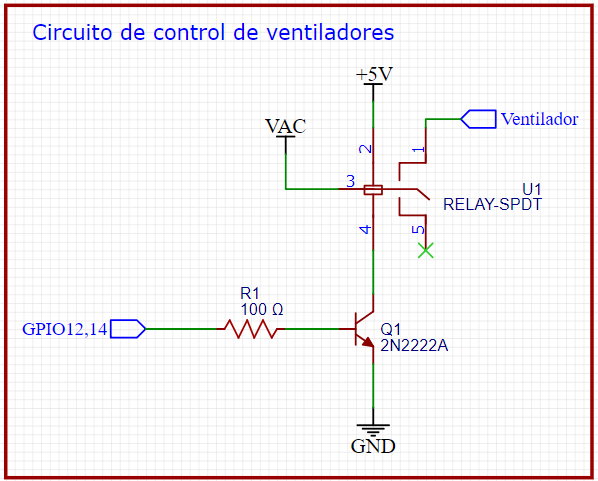
\includegraphics[scale= 0.4]{Circuito_ventiladores.png}
	\caption{Circuito con resistencia calculada para control de ventiladores con relés de 5 VCC.}
	\label{fig:diag_rele}
\end{figure}

Como se observa en el diagrama, los circuitos de control del ventilador inferior y superior se conectaron a los pines de uso múltiple 12 y 14 respectivamente. 

\subsubsection{Sensores de temperatura}

En el caso de los sensores de temperatura DHT11 y DS18B20, estos se conectaron según las recomendaciones del fabricante. Para los sensores DHT11 se utilizaron resistencias de $10k$ $\Omega$ conectadas entre 5 VCC y el pin de datos. Para estos sensores, se utilizaron los pines de uso general 4 y 13 del microcontrolador. Por otro lado, en los sensores DS18B20 se utilizó una única resistencia de $4.7k$ $\Omega$ conectada entre 5 VCC y el bus de datos. Debido al uso del protocolo One-wire, se utilizó un bus de datos conectado al pin de uso general número 15.

\subsubsection{Módulo RTC y luces de crecimiento}

El módulo de reloj de tiempo real DS3231 y las luces de crecimiento presentaron la conexión más sencilla. En estos componentes, no se utilizaron resistencias adicionales. En el caso del reloj de tiempo real, este se conectó a los pines de uso general 22 y 21, los cuales corresponden a la señal SCL y SDA respectivamente. Finalmente, las luces de crecimiento se conectaron al pin número 27.

\subsection{Desarrollo de placa PCB}			% [==========MISSING==========]

\section{Construcción del sistema}

Una vez completado el proceso de diseño general, se inició la construcción física del sistema. Como primer paso, se ensambló la estantería de metal, la cual sería utilizada como estructura principal para el sistema. Este proceso se logró con la ayuda de un mazo de goma y un metro, con los cuales se fijaron las repisas de la estantería a las alturas definidas en la etapa de diseño. Adicionalmente, se modificó una de las repisas con tal de asegurar un flujo adecuado de aire dentro del sistema. Estas modificaciones se realizaron utilizando un router manual con una fresa de 0.5 pulg con el cual se crearon ranuras longitudinales en la repisa de MDF. Una vez ensamblada la estructura principal, se inició con el ensamblaje de las tuberías de distribución y crecimiento.

El ensamblaje de las tuberías de crecimiento se inició con una tubería de 3 metros de largo, con un diámetro de 2 pulg. Esta tubería se cortó en las diferentes secciones requeridas para la construcción de los canales de crecimiento y tuberías de distribución. Luego, se utilizó una broca de copa de 1.5 pulg para realizar perforaciones en los canales de crecimiento espaciados a 17.54 mm. Estos agujeros serían utilizados para contener las plantas durante el período de crecimiento. Una vez se habían recortado todas las secciones de PVC, se utilizó sellador de silicona con una pureza del 100\% para unir las piezas con los codos y uniones tipo T. Se utilizó esta silicona para asegurar que no se encontraran fugas en los canales de distribución o crecimiento. Adicionalmente, la pureza aseguró que no se encontraran contaminantes los cuales podrían interferir con las pruebas a realizar. Finalmente, se conectó una manguera flexible de 0.5 pulg de diámetro interno al inicio de los canales de distribución, la cual permitiría suministrar el agua utilizando una bomba sumergible.

\subsection{Integración de sistemas}

Una vez se contaba con la estructura principal ensamblada, se inició la instalación de los diferentes componentes eléctricos y electrónicos en el sistema. Se instaló una caja plástica de 32 litros, la cual funcionaría como sistema de almacenamiento de agua. Una vez instalado dicho contenedor, se continuó con la instalación y conexión de sensores, actuadores, y la bomba sumergible.

\subsubsection{Conexión de sensores}

Tanto los sensores de temperatura ambiental como del agua requirieron de pequeñas modificaciones para su instalación. En el caso de los sensores DHT11, se crearon cables de conexión utilizando alambres de un cable UTP. Estos se unieron a terminales de pines axiales los cuales se utilizaron para conectar los cables a cada sensor y a la placa de desarrollo. Por otro lado, los sensores DS18B20 ya contaban con cables suficientemente largos, con la excepción de uno, por lo que se soldaron pines axiales directamente a los cables de los sensores. En el caso del sensor de temperatura de agua que se encontraba más alejado de la placa de desarrollo, se utilizó cable UTP para crear las extensiones requeridas. Finalmente, el sensor de pH SEN0161 cuenta con cables con terminales de pines axiales, por lo que la conexión no requirió de modificaciones a los cables existentes.

Los sensores DHT11 se instalaron utilizando las piezas impresas en 3D mencionadas al inicio del capítulo. Se utilizaron las varillas de 0.5 pulg para fijar los anillos de los sensores, y estas se insertaron directamente en la madera de las repisas. En el caso de las sondas de temperatura de agua, se introdujeron mediante los agujeros diseñados para fijar las plantas. Estas se ubicaron en cada una de las repisas de crecimiento, asegurando tomar mediciones en el punto de inicio del flujo de agua. La tercera sonda de temperatura de agua se instaló directamente en el depósito central de agua. 

\subsubsection{Instalación de bomba de circulación de agua}

La bomba de circulación de agua utilizada se acopló a la manguera flexible utilizando una boquilla de 0.5 pulg de diámetro, la cual se insertó a presión dentro de la manguera. Se aseguró que la distancia de la bomba hacia el punto de salida de la manguera se encontrara dentro de un rango de 3.5 pies, con tal de no forzar la bomba y asegurar un flujo adecuado de agua. Finalmente, la bomba se sumergió en el agua, y se fijó utilizando ventosas al fondo del depósito plástico. Se aseguró que la conexión del cable se encontrara lo más alejada de la fuente de agua posible, para evitar fallos por corto circuito.

\subsubsection{Instalación de actuadores}

Durante las primeras fases de construcción, se instalaron los ventiladores utilizando sus bases impresas, las cuales se fijaron mediante tornillos y tuercas a los perfiles de metal de la estructura principal. Al igual que los sensores, se soldaron extensiones de cable UTP a los ventiladores, permitiendo que los cables llegaran a sus puntos de conexión en la placa de desarrollo. Adicionalmente, se cubrieron todos los empalmes utilizando cinta de aislar, con tal de evitar fallos por corto circuito. Por otro lado, las luces de crecimiento se instalaron utilizando repisas adicionales, suspendidas a una distancia de aproximadamente 150 mm de las tuberías de crecimiento. Se utilizó cable UTP para unir las diferentes secciones de tiras LED, y se colocaron conectores axiales en cada una de las secciones, asegurando así una fácil conexión entre la placa de desarrollo y las luces de crecimiento.

\begin{figure}[H]
	\centering
	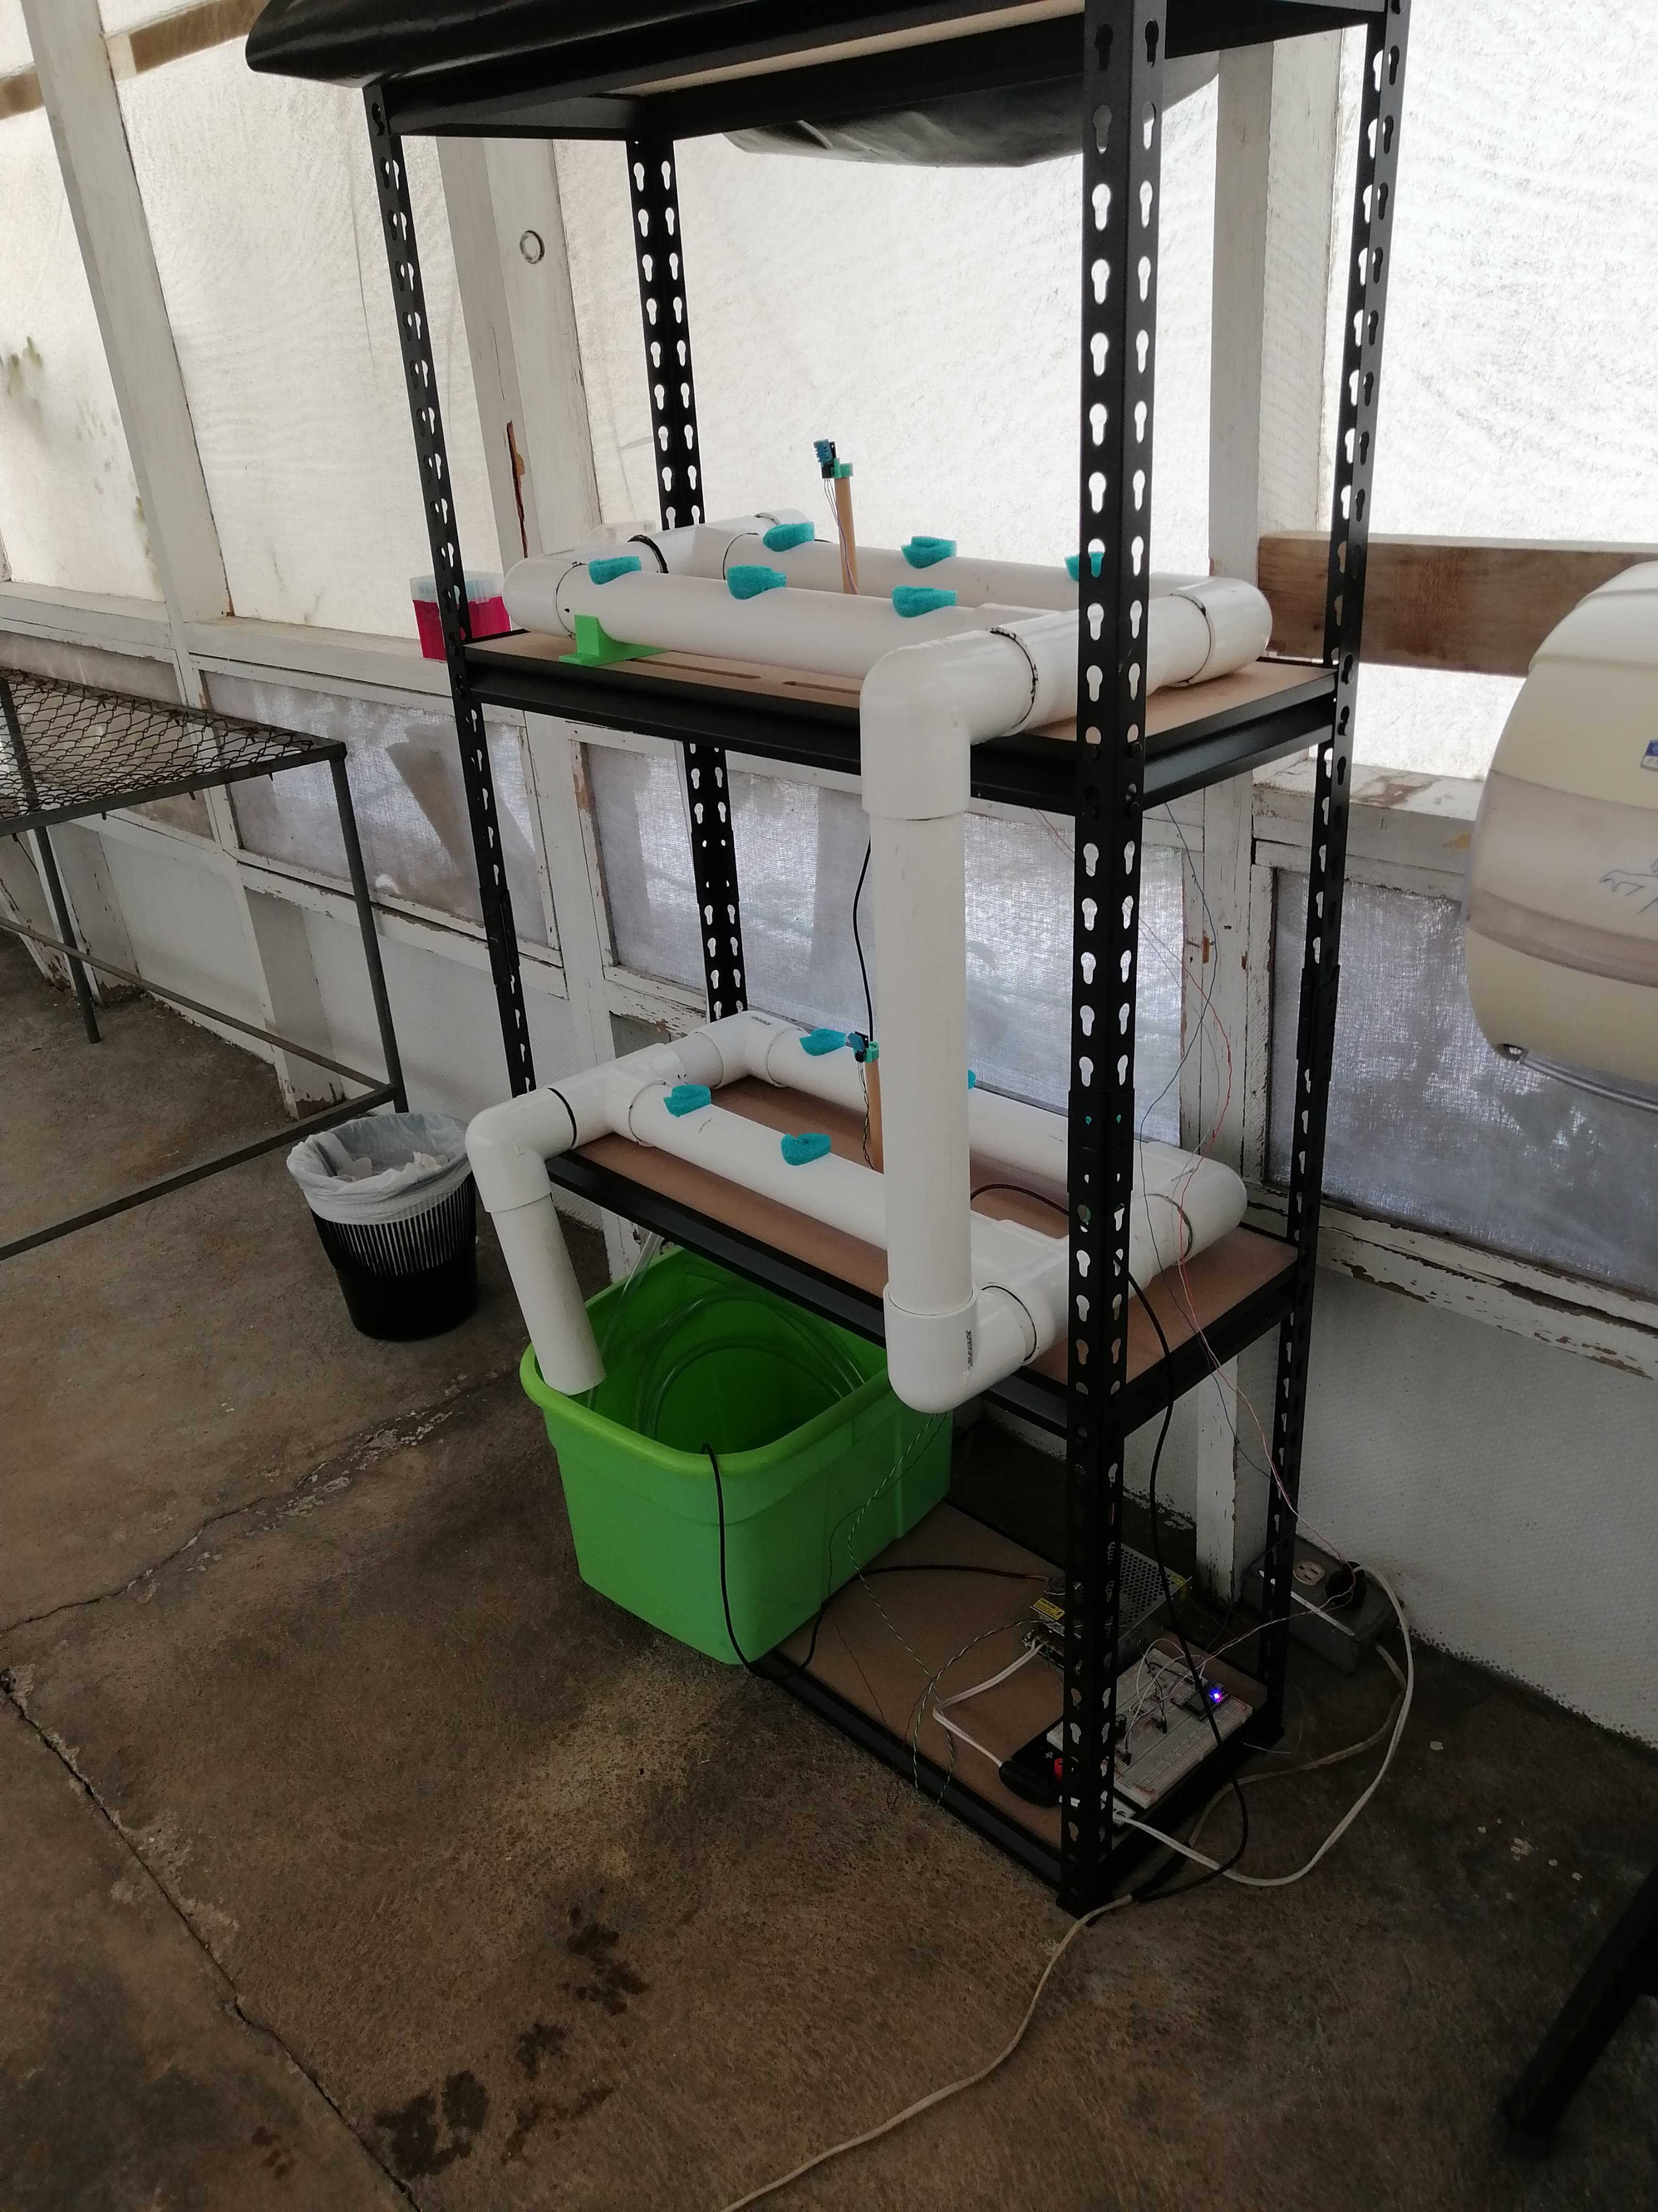
\includegraphics[scale= 0.05]{Estructura_principal.jpg}
	\caption{Estructura instalada en vivero con los diferentes componentes instalados y conectados.}
	\label{fig:estructura_final}
\end{figure}

%-----------------------------------------------------------------------------------------------------------

\chapter{Programación del \textit{firmware} del sistema}

\section{Definición de protocolo de comunicación inalámbrica}

Una de las ventajas de los sistemas hidropónicos se centra en sus bajos requisitos de mano de obra y atención constante. Esta ventaja se puede capitalizar significativamente al incluir un protocolo que permita enviar los datos a un servidor para ser consultados por un operador de manera remota. En el Siglo XXI, el crecimiento de tecnologías inalámbricas han facilitado esta tarea mediante el Internet de las cosas (IoT, por sus siglas en inglés). Si bien el internet de las cosas es un concepto sumamente valioso, este no se puede aprovechar sin contar con un protocolo de comunicación de datos que habilite su acceso.

\subsection{Conexión inalámbrica mediante WiFi}

El crecimiento en popularidad del internet de las cosas se atribuye principalmente a los avances realizados en cuanto a la familia de protocolos de comunicación con fidelidad inalámbrica, más conocida como WiFi. \cite{biber} Esta familia de protocolos ofrece una gran flexibilidad en cuanto a la estructura de paquetes para el envío de datos a través de grandes distancias y de una gran variedad de dispositivos. Esta versatilidad, permite a microcontroladores y plataformas de desarrollo como el ESP-WROOM32 utilizar este protocolo de comunicación para la transferencia de datos de manera inalámbrica.

Se utilizó la librería de \textit{WiFi.h} para la conexión del ESP-WROOM32 a una red local de internet. Una de las prioridades a la hora de diseñar la conexión a internet fue asegurar que el resto del sistema de control mantuviera su funcionamiento en caso de que se perdiera conexión WiFi. Tomando esto en cuenta, se estableció un intento inicial de conexión una vez se enciende el sistema. En caso de que se haya perdido conexión, o esta no se haya establecido exitosamente, se estableció un período de espera de 30 minutos, durante los cuales el sistema no intentaría conectarse al internet. Finalizados los 30 minutos, el sistema iniciaría nuevamente su rutina para establecer dicha conexión. Esta implementación fue esencial, puesto que la rutina para conectar el sistema al internet bloquearía el código durante un período considerable de tiempo. Por esta razón, sería necesario salir de la rutina de conexión luego de cierto tiempo, antes de volver a intentar la conexión.

\subsubsection{Protocolo HTTP}

Una vez establecida la conexión WiFi, se habilitó la comunicación con el servidro de Dweet.io mediante el protocolo HTTP. Puesto que la comunicación HTTP consiste de una solicitud enviada a un servidor, esta no requiere establecer una conexión como tal. Por esta razón, se programó una función a cargo de envíos de datos al servidor, iniciando la solicitud en el momento deseado, y finalizando una vez se recibió una respuesta adecuada del servidor. Debido a que una interrupción en el envío de datos podría resultar en un error, se estableció una cantidad de intentos máxima, para asegurar que los datos fuesen enviados, o que se regresara al ciclo principal en caso de no lograr la comunicación. Al igual que la función para la conexión a la red WiFi, la comunicación HTTP bloqueaba el código durante un tiempo significativo, por lo que estas medidas de seguridad se consideraron justificables.

Durante cada conexión al servidor, se enviaron dos paquetes de información, uno a la dirección \textit{hydro\_test} y otro a la dirección \textit{hydro\_LOG}. El primero de estos paquetes consistió de datos de los sensores, estados de los actuadores, e información de la fecha y hora del reloj de tiempo real del sistema. Esta información sería procesada por la aplicación con tal de monitorear los parámetros dentro del sistema de crecimiento. El segundo de los paquetes consistió de información acerca del estado de la conexión, detallando el nombre de la red a la que se encuentra conectado el sistema, así como la intensidad de la señal, la fecha y hora, y un contador de la cantidad de veces que falló el envío de datos al servidor antes del envío actual. Es importante mencionar que la información en ambos paquetes se configuró utilizando el formato JSON, el cual establece un objeto compuesto por un conjunto de propiedades, a las cuales se les asigna un valor según sea necesario. En este caso, se utilizó el formato JSON para establecer propiedades de temperatura, humedad, y otros parámetros los cuales se unieron con los valores recolectados por los sensores.

\section{Configuración de sensores y accionamiento de actuadores}

El proceso de configuración de los sensores de temperatura y humedad, así como las sondas de temperatura del agua, se completó sin mayor dificultad. Esto pues, la simplicidad en el funcionamiento de estos sensores eliminó los requerimientos de calibración. Los valores obtenidos de estos sensores se compararon con límites preestablecido, con tal de definir una secuencia de control sencilla para los ventiladores. Esto se implementó con tal de asegurar que tanto la temperatura como la humedad ambiental se mantuvieran en un rango adecuado para el crecimiento de las plantas. Por otro lado, los datos recolectados de las sondas de temperatura se almacenaron para ser enviadas al servidor de Dweet.io para su monitoreo.

En el caso de los actuadores, se establecieron funciones de control para los ventiladores y las luces de crecimiento respectivamente. En el caso de la función para la activación de los ventiladores, esta se enfocó en activar los pines transistorizados para cada ventilador, y cambiar el estado de banderas específicas con tal de comunicar el estado de los ventiladores al operador. Ahora bien, el control de las luces de crecimiento presentó una mayor cantidad de retos. Si bien la función diseñada para encender y apagar las luces de crecimiento no presentó grandes obstáculos, permitiendo cambiar el color de cada luz de manera individual y encender las luces a intervalos establecidos, se dificultó el registro del tiempo. Debido a los requerimientos de luz de las plantas, las luces de crecimiento deberían permanecer encendidas durante un período determinado. Ahora bien, se debería mantener un punto de referencia, con el cual se podría establecer cuánto tiempo han estado encendidas las luces, y cuanto tiempo más deberían estar apagadas, aún cuando el sistema de control perdiera alimentación. Por esta razón, se introdujo el módulo RTC, el cual aseguraría que las luces se encendieran siempre a la hora configurada, y se apagaran a la hora deseada. Durante la configuración del módulo RTC, se incluyó una rutina para sincronizar el tiempo del reloj interno con el tiempo del servidor de Dweet.io en caso de que el módulo perdiera poder. Estas medidas aseguraron que el tiempo del sistema se mantuviera de acuerdo con el tiempo real de la ubicación del sistema.

%------------------------------------------------------------------------------------------------------------

\chapter{Desarrollo de aplicación móvil}

\section{Requisitos de funcionalidad}

La aplicación móvil presenta una oportunidad de desarrollar una interfaz demostrativa, que sea capaz de brindar información al usuario de manera legible. Por esta razón, se establecieron diferentes requisitos de funcionalidad. Uno de estos, consistió en la conexión de la aplicación a internet para establecer una comunicación con el servidor de Dweet.io y obtener los datos del sistema. Otro de los requisitos de funcionalidad se centró en contar con una interfaz fácil de leer, que desplegara los datos recolectados por los sensores al usuario de una manera sencilla. De la mano con este requisito, se estableció que el usuario no fuese capaz de ingresar datos en las casillas que desplegaran los datos de los sensores. Finalmente, se buscó que la interfaz contara con un botón que permitiera al usuario refrescar los datos con tal de asegurar que la lectura más actualizada de los sensores se estuviese desplegando en la interfaz. 

\subsection{Diseño de interfaz gráfica}

El diseño de la interfaz gráfica se llevó a cabo utilizando el lenguaje de marcado extensible XML. Dentro del entorno de programación del estudio de \textit{Android}, se definieron dos pantallas. Una de estas presentaría el logo de la aplicación, así como el nombre, mientras que la segunda contaría con la información de los sensores del sistema. Se desarrolló el logo de la aplicación utilizando la herramienta gratuita de \textit{Canva}, y se utilizaron las herramientas de \textit{Android} para importar las imágenes utilizadas en la aplicación. Una vez se definieron las pantallas, sus estructuras y sus componentes, se continuó con la programación del funcionamiento de la aplicación.

\begin{figure}[H]
	\centering
	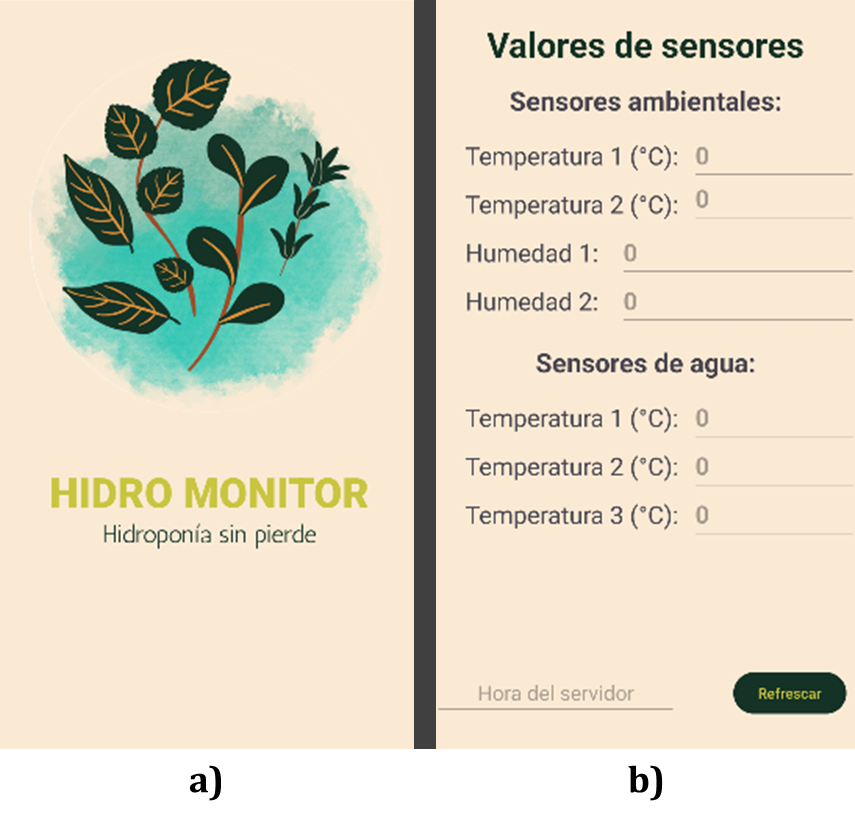
\includegraphics[scale= 0.5]{Interfaz_grafica.png}
	\caption{a) Pantalla de inicio de la aplicación. b) Interfaz gráfica principal.}
	\label{fig:interfaz_graf}
\end{figure}

\subsection{Lectura de datos de servidor HTTP}

Se utilizó el protocolo HTTP para obtener los datos del servidor Dweet.io bajo la dirección de \textit{hydro\_test}. Dentro de la función de lectura de datos del servidor, se obtuvieron los valores de las categorías del objeto JSON, y se asignaron a variables las cuales serán utilizadas para actualizar las casillas respectivas en la interfaz. Adicionalmente, se estableció un ciclo de lectura continuo, el cual realizaría una solicitud de información al servidor cada 5 minutos, e iniciaría un segundo después de acceder a la interfaz. Finalmente, se incluyó una función que ejecutaría una solicitud al servidor en el caso de que se presionara el botón para refrescar los datos.

\subsection{Notificaciones}					% [==========MISSING==========]

%-------------------------------------------------------------------------------------------------------------

\chapter{Evaluación del crecimiento del cilantro}

\section{Cultivo del cilantro en sustrato nutritivo}

Con tal de evaluar el crecimiento del cilantro, se inició un cultivo utilizando un sustrato activo. Este cultivo funcionaría como punto de comparación, permitiendo identificar cambios en el crecimiento del cilantro dentro del sistema. Con tal de lograr el crecimiento adecuado de las plantas de cilantro, se estableció un sustrato que fuese capaz de cumplir con las siguientes características: alta retención de humedad, baja densidad permitiendo oxigenación y un alto contenido nutritivo. Con estas características en mente, se realizó una mezcla de vermiculita, \textit{peat-moss}, tierra abonada y compost orgánico. Esta mezcla permitió contar con una buena retención de agua gracias a la vermiculita, un nivel bajo de densidad debido al \textit{peat-moss}, y una alta cantidad de nutrientes. Una vez se preparó el sustrato de crecimiento, se repartió en diferentes contenedores, los cuales permitirían el desarrollo de las plantas asegurando una distancia de 180 mm entre planta. 

\subsection{Período de germinación del cilantro}

Con tal de establecer una línea base de crecimiento, se inició un grupo de plantas de cilantro desde la semilla. Para esto, se emplearon dos metodologías de germinación. En la primera, como se observa en la Figura \ref{fig:ziplock} se utilizó una bolsa resellable, en la cual se introdujo una toalla de papel húmeda con semillas de cilantro. Esta bolsa se almacenó en un ambiente oscuro y a una temperatura constante cercana a los 25 °C. Como segundo método, se utilizó un sustrato inerte, el cual consistió en una mezcla de \textit{peat-moss}, vermiculita y fibra de coco como sustrato de germinación. 

\begin{figure}[H]
	\centering
	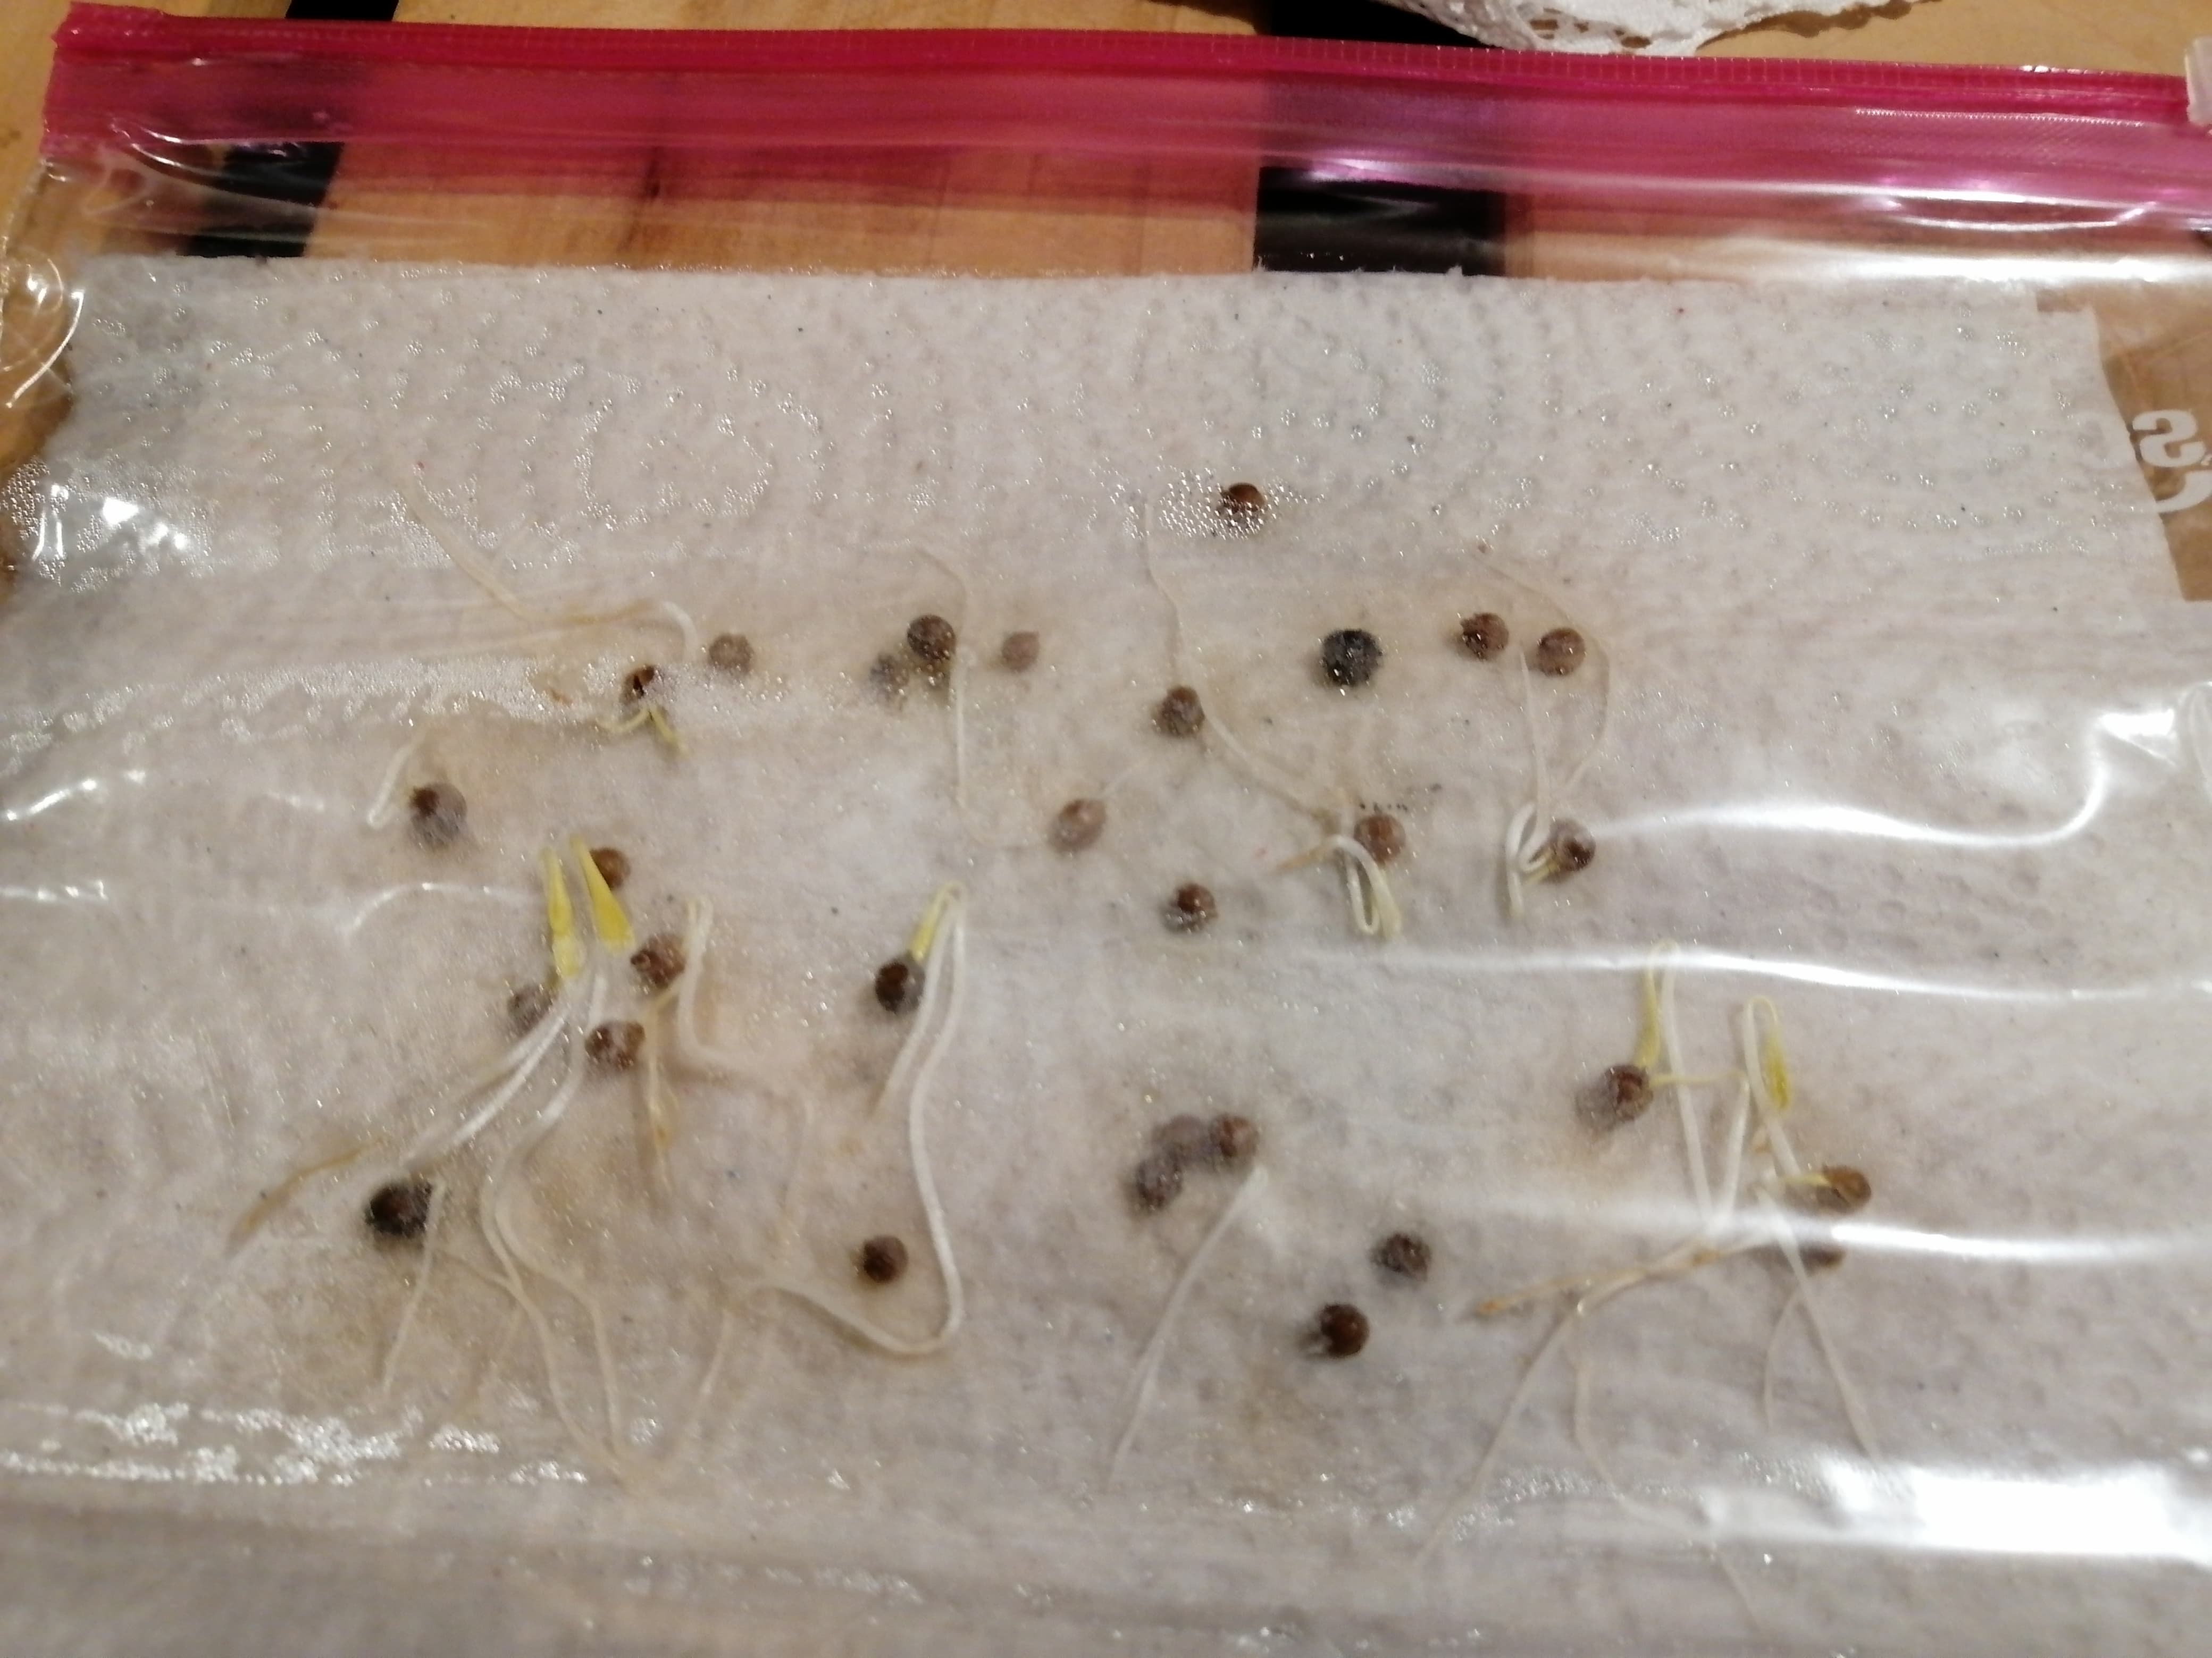
\includegraphics[scale= 0.05]{Germinacion_ziplock.jpg}
	\caption{Semillas germinadas utilizando papel toalla y bolsa resellable.}
	\label{fig:ziplock}
\end{figure}

\begin{figure}[H]
	\centering
	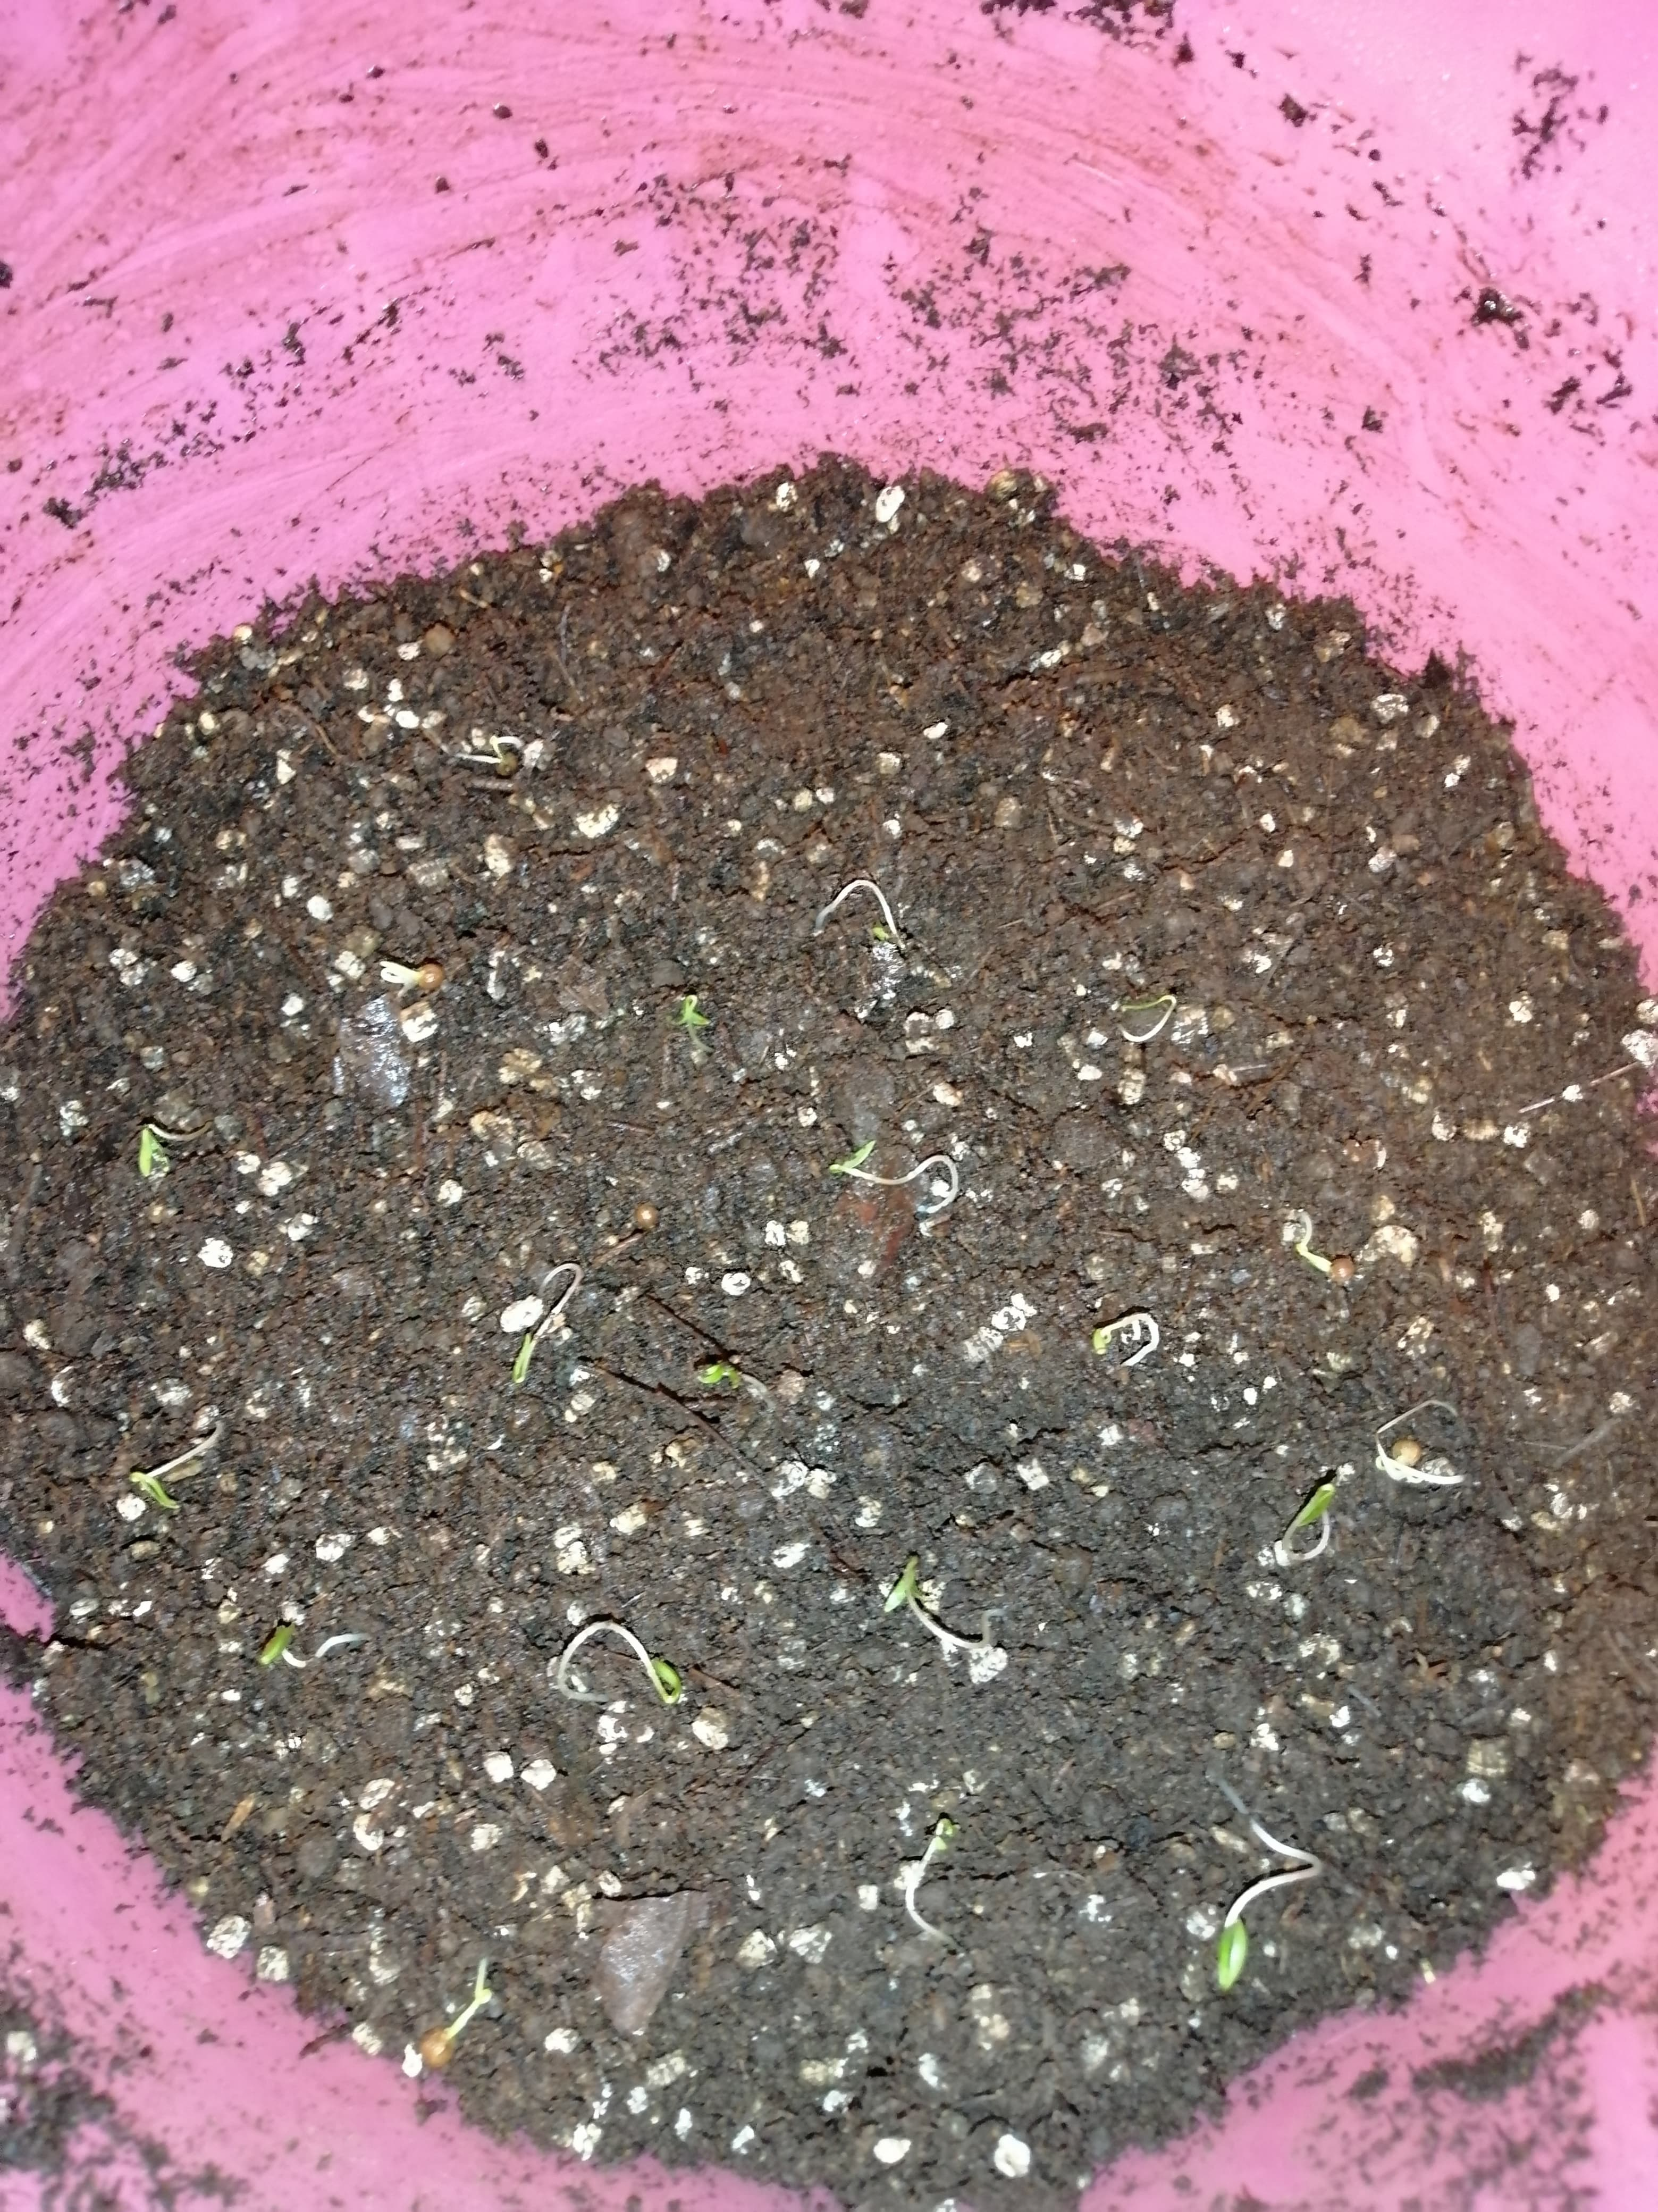
\includegraphics[scale= 0.05]{Germinacion_peatmoss.jpg}
	\caption{Semillas germinadas utilizando sustrato mecánico inerte.}
	\label{fig:peatmoss}
\end{figure}

Tanto las semillas en la bolsa resellable como las del sustrato inerte presentaron desarrollo de raíces luego de 8 días en condiciones óptimas. Es importante mencionar que si bien el sustrato inerte fue capaz de mantener un nivel de humedad aceptable, fue necesario regar dicho sistema de manera periódica durante el tiempo de germinación. Por otro lado, las semillas dentro de la bolsa resellable nunca presentaron pérdidas significativas de humedad, por lo que no fue necesario hidratarlas más de una vez. A parte de la diferencia en retención de humedad, no se observó una diferencia significativa entre ambos métodos de germinación en cuanto al tiempo o eficiencia. 

\subsection{Retos en el desarrollo de retoños}

Una vez se observó el desarrollo de raíces en los retoños, estos se trasladaron a un sustrato compuesto principalmente por \textit{peat-moss}, vermiculita y tierra abonada. Es importante resaltar que durante las primeras semanas de desarrollo, los retoños no recibieron una cantidad adecuada de luz, por lo que se presentó un fenómeno conocido como \textit{bolting} o espigado. Este proceso llevó al desarrollo de tallos largos y débiles, lo cual llegó a representar un reto significativo en futuras etapas del desarrollo. Adicionalmente, durante las primeras semanas de crecimiento, se utilizó una proporción menor de compost, lo cual redujo la cantidad de nutrientes disponibles para los retoños.

\subsection{Transplante de retoños a sustrato nutritivo de crecimiento}

Los retos mencionados anteriormente se corrigieron luego de transplantar los retoños al sustrato nutritivo, sin embargo, la mayoría de los retoños contaban con un tallo principal considerablemente largo y débil. Por esta razón, se sembraron los retoños a una mayor profundidad, buscando evitar la pérdida de retoños por daños al tallo. Mientras que este proceso ayudó a que la mayoría de los retoños se continuaran desarrollando, la exposición a los elementos como la lluvia y el viento inevitablemente dobló algunos de los retoños, llevando a pérdidas por falta de circulación de nutrientes a través de los tallos. En la Figura \ref{fig:transplante_plantas}, se observa la configuración de los retoños en las macetas, y se acortó la altura de los tallos al sembrarlos a mayor profundidad. Finalmente, es importante mencionar que durante el proceso de transplante, se descartaron aquellos retoños que se habían vencido sobre su propio peso, así como retoños que no habían desarrollado suficientemente sus raíces como para absorber nutrientes del sustrato.

\begin{figure}[H]
	\centering
	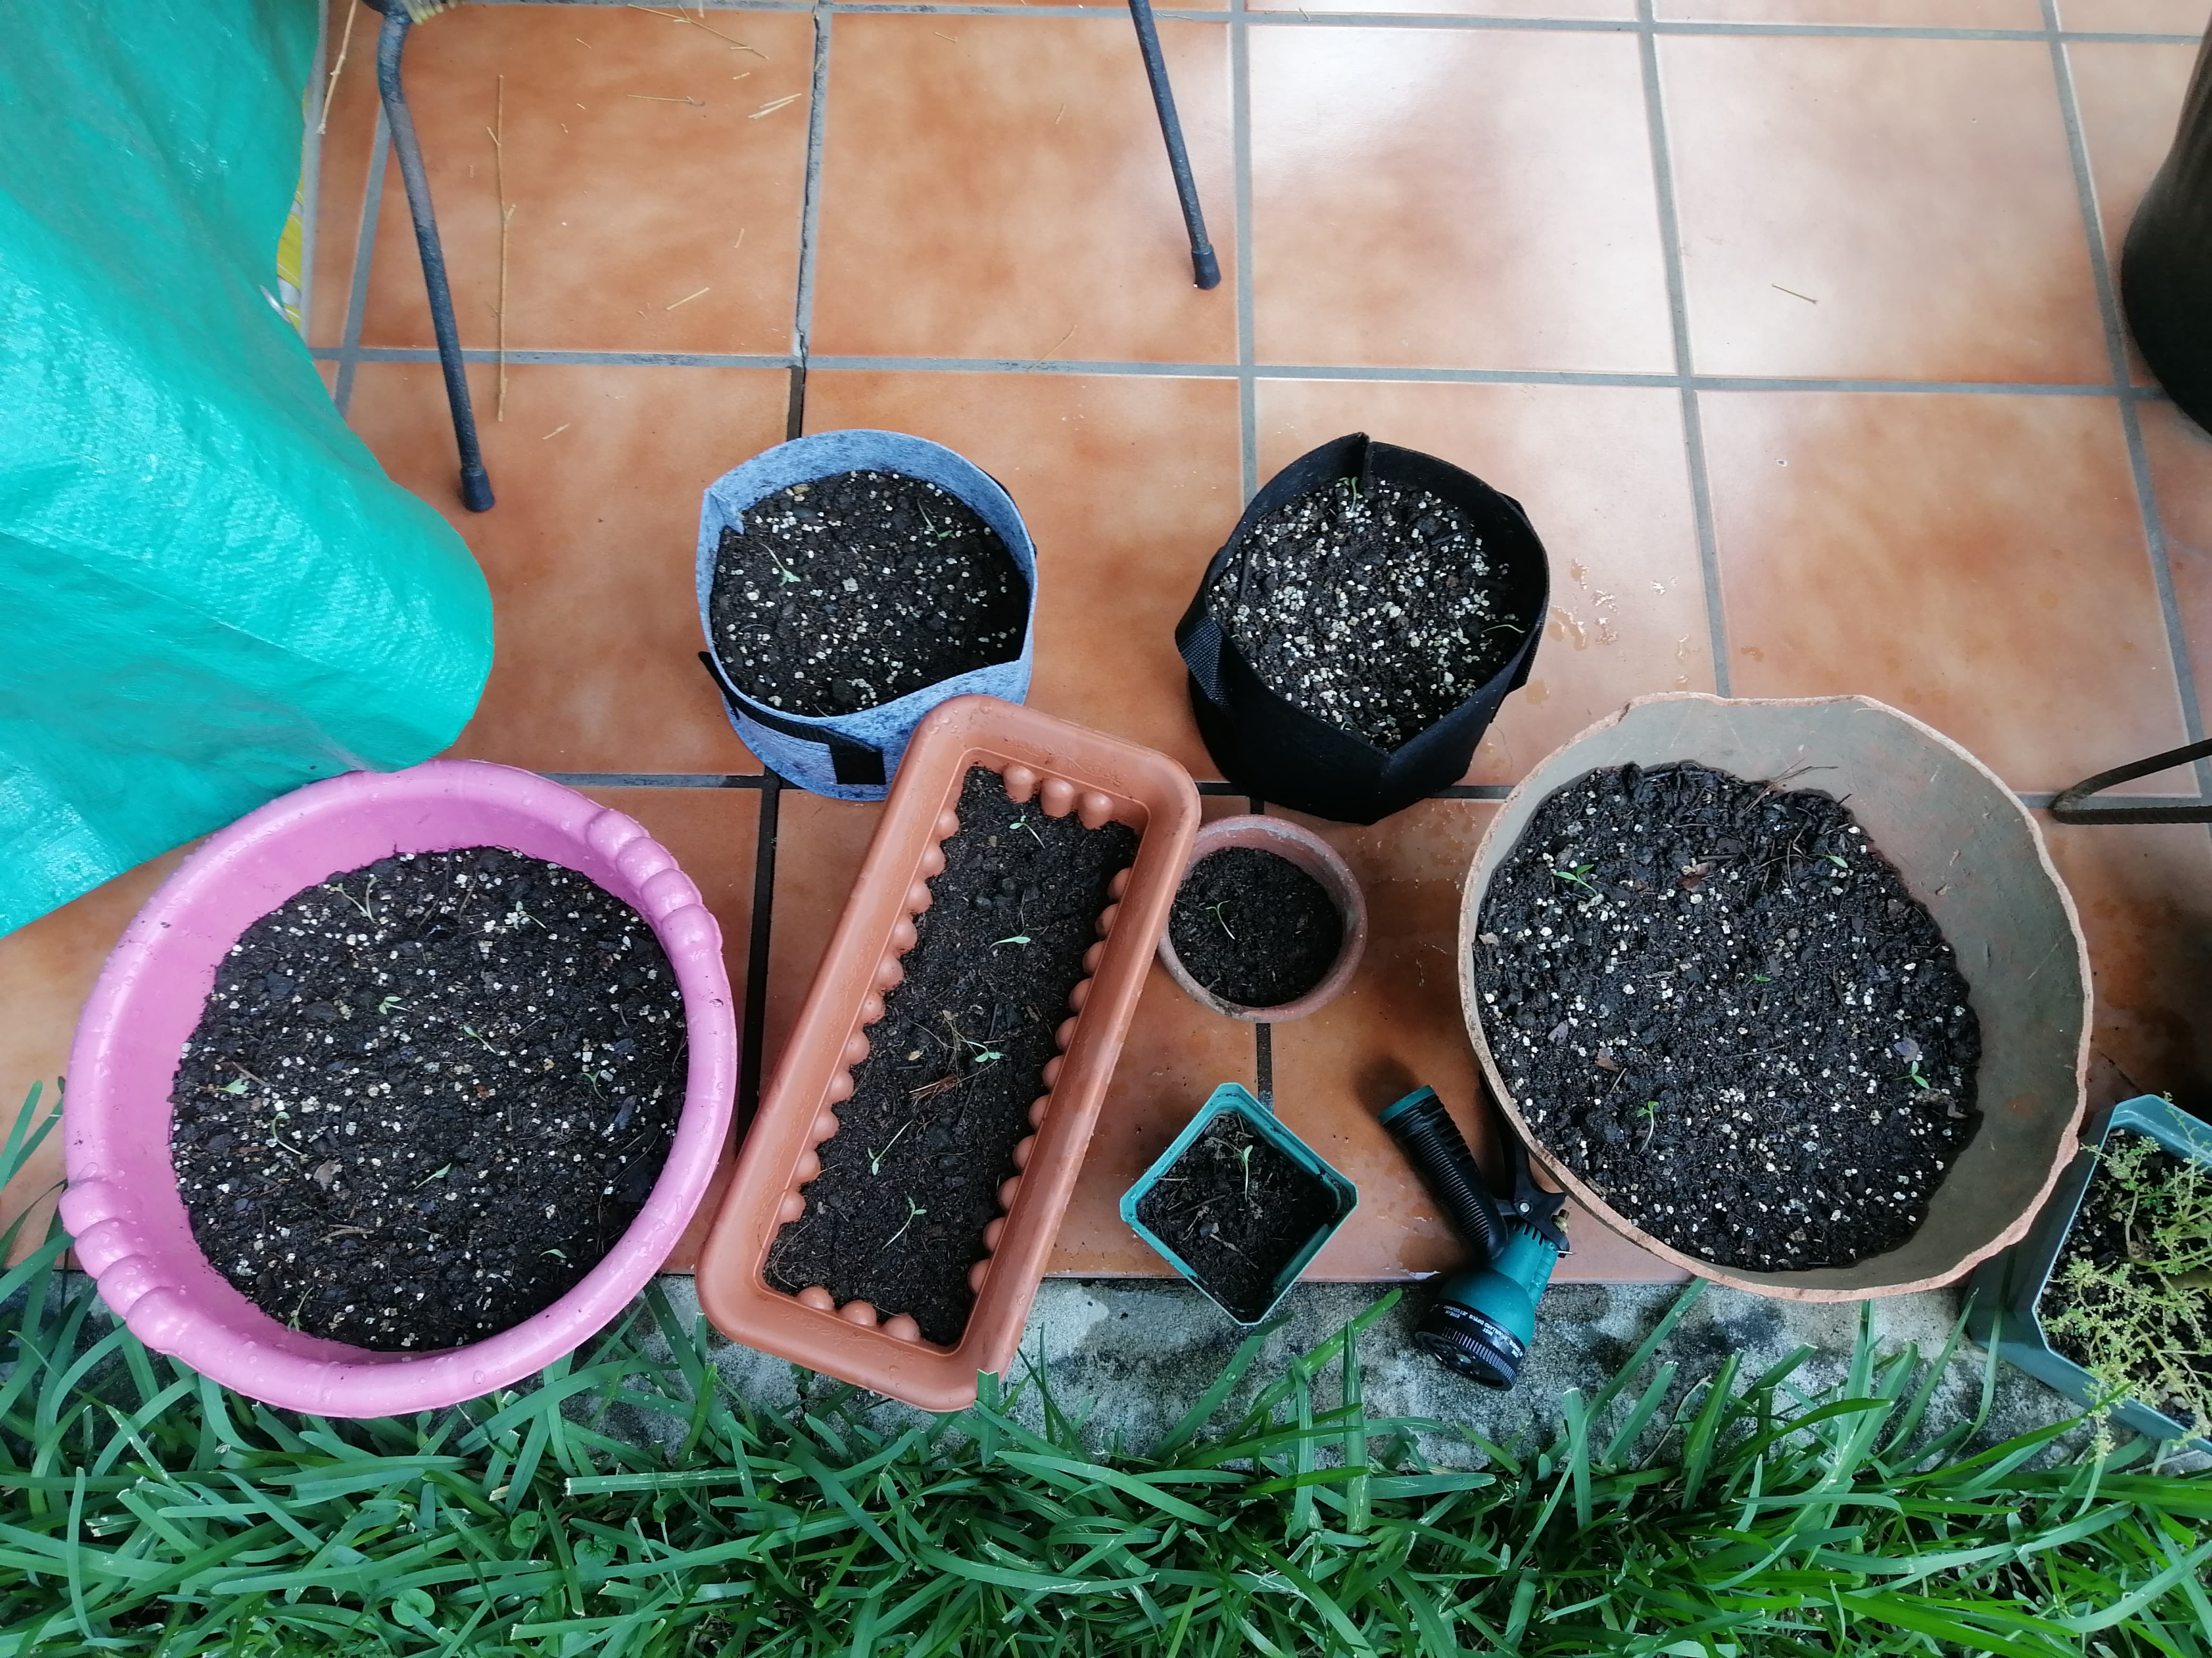
\includegraphics[scale= 0.05]{Retonos_transplantados.jpg}
	\caption{Configuración de los retoños luego de ser transplantados a sustrato nutritivo de crecimiento.}
	\label{fig:transplante_plantas}
\end{figure}


\section{Cultivo de cilantro en sistema hidropónico}

Luego de las primeras 4 semanas del desarrollo del cilantro en sustrato de crecimiento, se trasladaron 12 plantas de cilantro al sistema hidropónico. Se colocó una planta por espacio disponible en los canales de crecimiento, y se reguló la concentración de solución nutritiva, diluyendo 2.5 mL de macro y micro nutrientes por galón de agua en el sistema. Ahora bien, cabe mencionar que en el momento en que se trasladaron las plantas de cilantro, aún no se contaba con un control adecuado de temperatura ambiente. Adicionalmente, como se observa en la Figura \ref{fig:estructura_final}, el sistema tampoco contaba con un control de luz de crecimiento, estando abierto aún a la luz ambiental.

\subsection{Elementos de soporte para las plantas}

En un sustrato activo, este provee tanto los nutrientes necesarios para el crecimiento de las plantas, como la estabilidad mecánica para asegurar que estas se mantengan erguidas. Ahora bien, en un sistema hidropónico, las plantas no cuentan con este sustrato, por lo cual es necesario utilizar otros métodos para brindar estabilidad mecánica a las plantas. Durante las pruebas iniciales, se utilizaron pedazos de tubo flotador, los cuales se cortaron de manera que fuesen capaces de ingresar en los agujeros disponibles en los canales de crecimiento. Además, se aseguró que estos fueran capaces de apoyar a las plantas, asegurando que se mantuvieran en su lugar. Ahora bien, cabe mencionar que estos tubos flotadores están elaborados de un material sintético el cual absorbe e irradia calor con facilidad. Esto no habría sido un gran problema en un sistema hidropónico sumergible, sin embargo, al utilizar la metodología NFT, este material no contó con una manera de liberar su calor.

Mientras se realizaron pruebas iniciales de crecimiento, se observó una temperatura máxima en el sistema alrededor de los 32 °C, la cual fue considerablemente mayor a la temperatura máxima del cilantro, alrededor de los 25 °C. Este aumento en temperatura elevó el consumo de agua de las plantas, resultando en una acumulación de sales en las raíces, como se observa en la Figura \ref{fig:raices}. Esta acumulación de sales, junto a las elevadas temperaturas en los pedazos de tubo flotante, llevaron a la pérdida del 66\% de las plantas en el sistema hidropónico.

\begin{figure}[H]
	\centering
	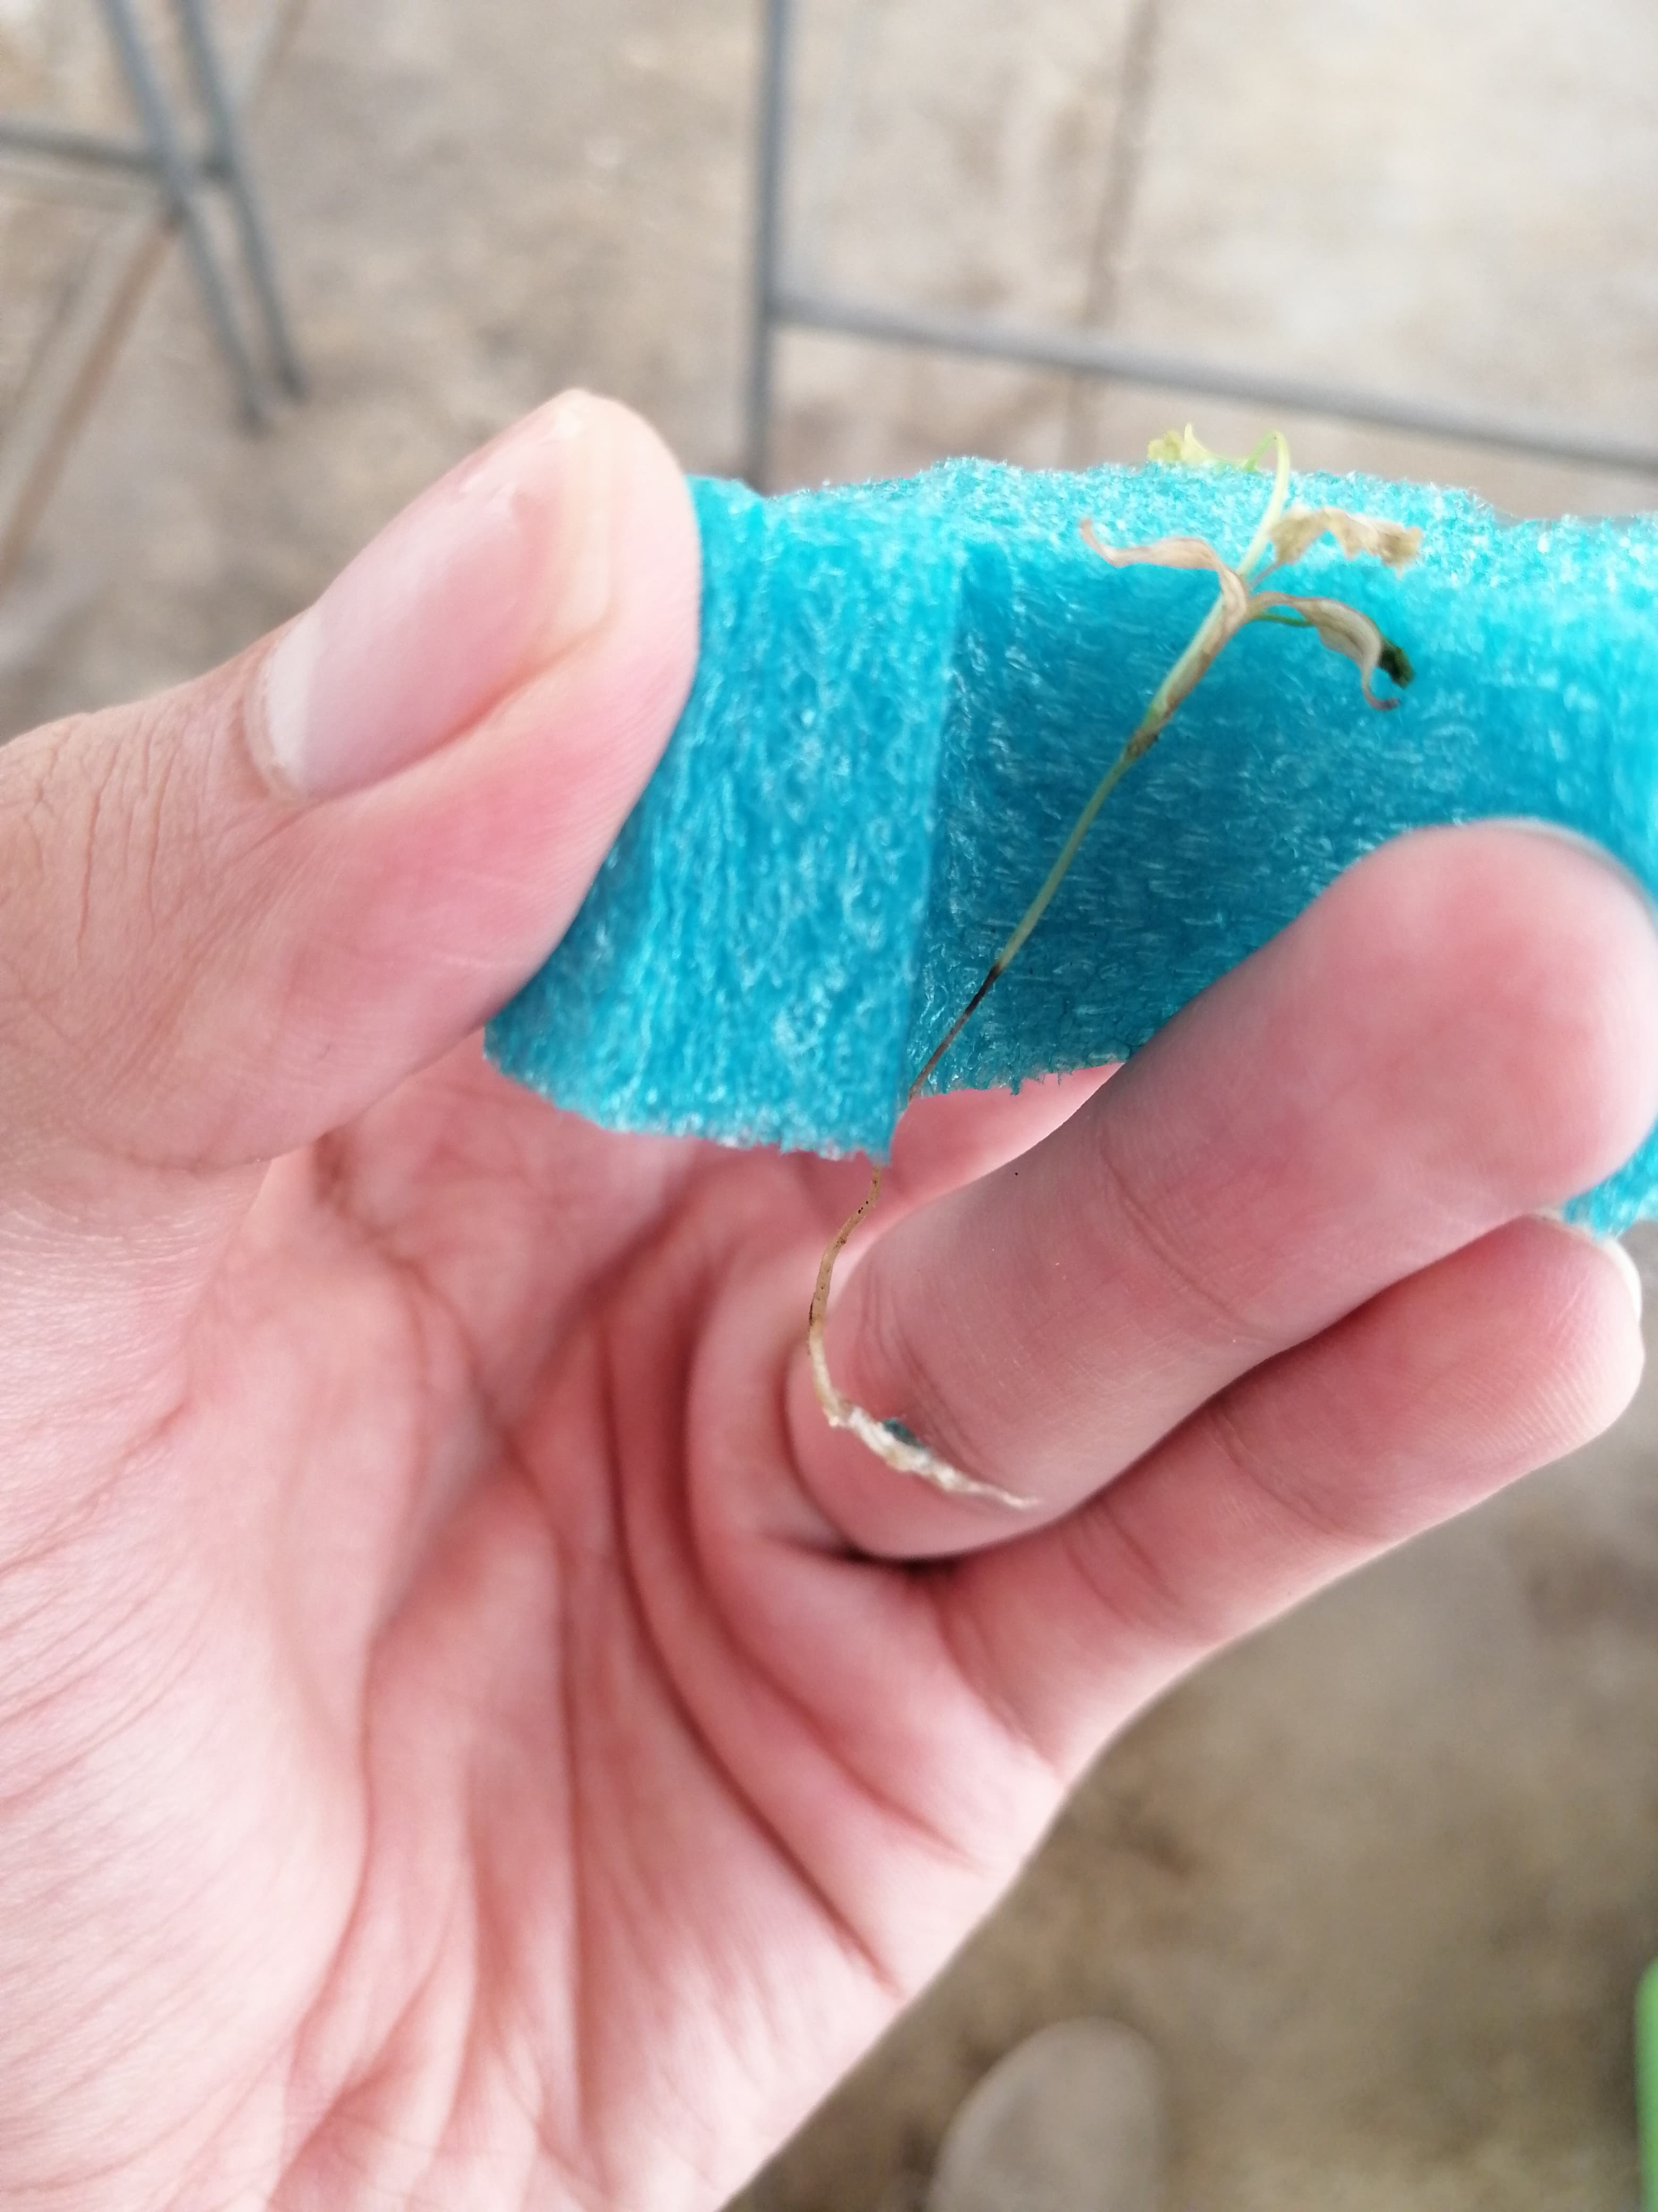
\includegraphics[scale= 0.05]{Sales_raices.jpg}
	\caption{Retoño de cilantro con tallo seco y raíces bloqueadas por sales de la solución nutritiva.}
	\label{fig:raices}
\end{figure}

\section{Retos en el cultivo del cilantro durante períodos de prueba}	% [==========MISSING==========]

\section{Comparaciones del crecimiento del cilantro}	% [==========MISSING==========]


\fi

% CONCLUSIONES
% ------------------------------------------------------------------------------
\ifdefined\CAPconclusiones
	\newpage
	\chapter{Conclusiones}
	\ifdefined\parpordefecto
		\defaultparformat{k-conclusiones}
	\else
		\input{k-conclusiones}
	\fi
\fi

% RECOMENDACIONES
% ------------------------------------------------------------------------------
\ifdefined\CAPrecomendaciones
	\newpage
	\chapter{Recomendaciones}
	\ifdefined\parpordefecto
		\defaultparformat{l-recomendaciones}
	\else
		A lo largo de las diferentes etapas de desarrollo de este proyecto de graduación, se identificaron diferentes características que se deben considerar a la hora de continuar con el desarrollo del sistema. Si bien estas características no afectaron directamente el funcionamiento principal del sistema, se consideró que su implementación facilitaría considerablemente el proceso de desarrollo, construcción, y resultados finales del trabajo. A continuación se encuentra un listado de las recomendaciones principales del presente trabajo de graduación.

\begin{itemize}
	\item Emplear una combinación de dos microcontroladores, dedicando uno al análisis y manejo de datos y el segundo a el control de sensores y actuadores con tal de reducir la carga del firmware sobre el microcontrolador.
	\item Utilizar un sistema de ventilación más robusto que asegure un mejor flujo de aire y permita regular la temperatura del sistema tanto para enfriar como para calentar el entorno.
\end{itemize}
	\fi
\fi

% BIBLIOGRAFÍA
% ------------------------------------------------------------------------------
\ifdefined\CAPbibliografia
	\newpage
    \cleardoublepage\phantomsection
	\chapter{\bibname}
    \printbibliography[heading=none]
\fi

% ANEXOS
% ------------------------------------------------------------------------------
\ifdefined\CAPanexos
	\newpage
	\chapter{Anexos}
	\ifdefined\parpordefecto
		\defaultparformat{n-anexos}
	\else
		\section{Planos de construcción}
	\fi
\fi

% GLOSARIO
% ------------------------------------------------------------------------------
\ifdefined\CAPglosario
	\newpage
	\printglossary
\fi

\end{document}